\onehalfspace

\include{preface}

\chapter*{Contributors to this article}

\section*{Content}

\begin{itemize}
\item Ramprasad Saptharishi (Tel Aviv University)

\texttt{ramprasad@cmi.ac.in}

\item Suryajith Chillara (Chennai Mathematical Institute)

\texttt{suryajith@cmi.ac.in}

Parts of \autoref{chap:dc}


\item Mrinal Kumar (Rutgers University)

\texttt{mrinal.kumar@rutgers.edu}

\autoref{chap:lowAlgRank}

\item Anamay Tengse (Tata Institute of Fundamental Research)

\texttt{tengse.anamay@tifr.res.in}

\autoref{chap:DMPY}

\end{itemize}

\section*{Corrections, minor edits}

\begin{itemize}
\item V Vinay (Limberlink Technologies)

\texttt{vinay@jed-i.in}

\item Noam Mazor (Tel Aviv University)

\item Amir Shpilka (Tel Aviv University)

\texttt{shpilka@post.tau.ac.il}

\item Anamay Tengse (Tata Institute of Fundamental Research)

\texttt{tengse.anamay@tifr.res.in}

\item Suhail Sherif (Tata Institute of Fundamental Research)

\texttt{suhail.sherif@gmail.com}

\item \texttt{Christian Engels}

  \url{https://github.com/Narfinger}

\item Prateek Dwivedi

  \url{https://github.com/prateekdwv}

\item Prerona Chatterjee

  \url{http://www.tifr.res.in/~prerona.chatterjee/}

\item \texttt{anag004@github}

  \url{https://github.com/anag004}

\item Srikanth Srinivasan

  \url{Aarhus University}

\end{itemize}


%%% Local Variables:
%%% mode: latex
%%% TeX-master: "fancymain"
%%% End:


% \hypersetup{
%   linkcolor={DarkSlateGray}
% }
\tableofcontents

\include{dependencies}

\chapter{Introduction}\label{chap:intro}


``What is the best way to compute a given polynomial $f(x_1,\dots, x_n)$ from basic operations such as $+$ and $\times$?'' This is the main motivating problem in the field of arithmetic circuit complexity. 
The notion of \emph{complexity} of a polynomial is measured via the size of the smallest arithmetic circuit computing it. 
Arithmetic circuits provide a robust model of computation for polynomials. 
Formally, these are directed acyclic graphs with a unique sink vertex, where internal nodes are labelled by $+$ and $\times$ and each source node labelled with either a variable or a field constant. 
Each $+$ gate computes the sum of the polynomials computed at its children, and $\times$ gates the product. 
The unique sink vertex is called the root or the output gate, and the polynomial computed by that gate is the polynomial computed by the circuit. 

There are several interesting questions that can be asked about arithmetic circuits, and polynomials that they compute. 
One category of problems are of the form, ``Is there an explicit polynomial $f(x_1,\dots, x_n)$ that require (perhaps restricted) arithmetic circuits of size $2^{\Omega(n)}$ to compute them?'', or questions about proving lower bounds. 
Another category of problems are of the form, ``Is the given circuit computing the $0$ polynomial?'', which is also called `Polynomial Identity Testing (PIT)'. 
Yet another class of questions are of the form ``Given oracle access to a circuit, can you write down the polynomial computed by this circuit?'', which are also called `polynomial reconstruction'. 
Several of these problems have very strong connections between each other despite being of very different flavours. 
Formal connections between PIT and lower bounds have been shown by \cite{ki03,a05}. 
Further, strong lower bounds for restricted models have often been succeeded by reconstruction algorithms (at least on average). 
In this article we shall mainly be looking at lower bounds. 
For more on reconstruction and PIT questions, the author is invited to read other excellent surveys such as \cite{sy,ckw11}. 

\section{Arithmetic complexity classes}
In the seminal paper of \cite{v79}, Valiant defined two classes of polynomials which we now call $\VP$ and $\VNP$. 

\begin{definition}
The class $\VP$ is defined as the set of all polynomial $f(x_1,\dots, x_n)$ with $\deg(f) = n^{O(1)}$ that can be computed by an arithmetic circuit of size $s = n^{O(1)}$. 

The class $\VNP$ is defined as the set of all polynomial $f(x_1,\dots, x_n)$ such that there exists a $g(x_1,\dots, x_n, y_1,\dots, y_m) \in \VP$ with $m = n^{O(1)}$ such that
\[
f(x_1,\dots, x_n) \quad = \quad \sum_{y_1=0}^1\dots \sum_{y_m=0}^1 g(x_1,\dots, x_n, y_1,\dots, y_m).
\]
\end{definition}
The class $\VP$ is synonymous to what we understand as \emph{efficiently computable} polynomials. 
The class $\VNP$, whose definition is similar to the boolean class $\NP$, is in some sense a notion of what deem as \emph{explicit}. 

\begin{fact}
Let $f(x_1,\dots, x_n)$ be a polynomial such that $\deg(f) = n^{O(1)}$ and given any exponent vector $e_1,\dots, e_n$, the coefficient of the monomial $x_1^{e_1}\dots x_n^{e_n}$ in $f$ can be computed in polynomial time. 
Then, $f \in \VNP$. 
\end{fact}

For example, consider the permanent of a symbolic $n\times n$ matrix. 
In fact, \cite{v79} showed that the symbolic $n\times n$ permanent is in some sense complete for the class $\VNP$. 
Further, he also showed that the determinant of a symbolic  $n\times n$ matrix is (almost) complete for the class $\VP$. 
Separating the determinant and the permanent is the Holy Grail in the field of arithmetic circuit complexity. \\

{\bf Remark.} Note that the above fact merely gives a sufficient condition for a polynomial to be in $\VNP$. 
There are examples of polynomials $f$ where computing the coefficient of a given monomial is believed to be very hard but $f\in \VNP$.\footnote{For example, consider the $n^2$ variate multilinear polynomial $f$ such that the coefficient $x_{11}^{e_{11}}\dots x_{nn}^{e_{nn}}$ is the permanent of the $n\times n$ matrix $(\!(e_{ij})\!)_{i,j}$. 
Turns out $f \in \VNP$. 
In fact, a necessary and sufficient condition is that the coefficient of a given monomial can be computed in $\#\mathsf{P}/\poly$. }  In this article however, all the polynomials we shall be dealing with would have this property that the coefficient of a given monomial can be efficiently computed. 
For more about completeness classes in arithmetic complexity, \cite{bcs97} is a wonderful text. 


\section{Prior lower bounds}

Proving lower bounds is generally considered challenging, in most models of computation. 
For general circuits, the best lower bound we have for an explicit polynomial is by \cite{BS83} who prove an $\Omega(n\log n)$ lower bound. 
For the subclass of arithmetic formulas, \cite{k85} has shown a $\Omega(n^{3/2})$ lower bound. 
On the other hand, we know by standard counting methods that most $n$-variate degree $d$ polynomials require circuits of size $\Omega\inparen{\sqrt{\binom{n+d}{d}}}$.

To gain better understanding of computation by arithmetic circuits, researchers focused on proving lower bounds for restricted models of computation. 
One very natural restriction is the depth of the circuit. 
Proving lower bounds for depth two circuits are trivial. 
For general depth three circuits, the best lower bound we have is by \cite{sw2001} who present an $\Omega(n^2)$ lower bound. 
Exponential lower bounds are known with additional restrictions like \emph{homogeneity} \cite{nw1997}, \emph{multilinearity} \cite{raz2004,raz-yehudayoff}, over finite fields \cite{gr00,grigoriev98}, \emph{monotonicity} \cite{js82} etc. 

For multilinear models, more is known for even larger depth. \cite{raz2004} showed an $n^{\Omega(\log n)}$ lower bound for the class of multilinear formulas. \cite{raz-yehudayoff} extended those techniques to show an $2^{n^{\Omega(1/\Delta)}}$ lower bound for multilinear formulas of depth $\Delta$. 

\section{Relevance of shallow circuits for ``$\VP$ vs $\VNP$''}

The study of lower bounds for shallow circuits is not just an attempt to simplify the problem and gain insight on the larger goal. 
The class of shallow arithmetic circuits are surprisingly powerful, unlike the boolean case. 
Shallow circuits in the arithmetic world almost capture the entire computational power of unrestricted circuits! 

There has been a long series of results that simulate a general arithmetic circuit $C$ by a \emph{shallow} circuit of size comparable to the size of $C$. 
This task simulating a circuit with another not-too-large circuit of small depth is called \emph{depth reduction}. 
The first result in this regard is by \cite{vsbr83} who proved the following. 

\begin{theorem}[\cite{vsbr83}]
Let $f$ be an $n$-variate degree $d$ polynomial computed by an arithmetic circuit $C$ of size $s$. 
Then, $f$ can be equivalently computed by a homogeneous circuit $C'$ of depth $O(\log d)$ with unbounded fan-in $+$ and $\times$ gates and size $s' = (nds)^{O(1)}$. 
\end{theorem}


The above theorem allows us to focus on just homogeneous circuits of $O(\log d)$ depth and attempt lower bounds for this model. 
Any super-polynomial lower bound for the class of $O(\log d)$ depth circuits automatically yields a super-polynomial lower bound for general circuits. \\

However, if we really hope to prove much stronger lower bounds for $\Perm_n$ like say $2^{\Omega(n)}$, maybe we can afford to incur a slightly larger blow-up in size to obtain an even shallower circuit. 
This line was first pursued by \cite{av08}, and subsequently strengthened by \cite{koiran} and \cite{Tav13} to yield the following result. 

\begin{theorem}[\cite{av08,koiran,Tav13}] 
  Let $f$ be an $n$-variate degree $d$ polynomial computed by an arithmetic circuit of size $s$. 
Then $f$ can be computed by a homogeneous $\SPSPfanin{O(\sqrt{d})}{\sqrt{d}}$ circuit of size $s' \leq s^{O(\sqrt{d})}$

More generally, for any $0\leq r\leq d$, there is a homogeneous $\SPSPfanin{O(d/r)}{r}$ circuit of top fan-in at most $s^{O(d/t)}$ computing $f$. 
\end{theorem}

Recall that a $\SPSPfanin{O(\sqrt{d})}{\sqrt{d}}$ circuit computes a polynomial of the form
\[
f\spaced{=} \sum_{i=1}^s Q_{i1}\dots Q_{ia},\quad \text{where $a = O(\sqrt{d})$ and $\deg Q_{ij} \leq \sqrt{d}$}.
\]

In other words, if we can prove a lower bound of $n^{\omega(\sqrt{d})}$ for the class of $\SPSPfanin{O(\sqrt{d})}{\sqrt{d}}$ circuits, we would have a super-polynomial lower bound for the class of general arithmetic circuits! 
In fact, the model of depth $4$ circuits seem so central in that almost all known lower bounds for other restricted models proceed by proving a suitable lower bound for a depth $4$ analogue. 
Several examples of this may be seen in \cite{KayalRP}. \\

The first breakthrough was obtained by \cite{gkks13} who showed an $2^{\Omega(\sqrt{d})}$ lower bound for such circuits computing the symbolic $d\times d$ determinant or permanent. 
Subsequently, there was a flurry of activity towards achieving the goal of proving $n^{\omega(\sqrt{d})}$ lower bounds \cite{KSS13,FLMS13,KS14a}, and this is where we currently stand. 

\begin{theorem}
There is an explicit homogeneous $n$-variate degree $d$ polynomial $f$ that can be computed by a homogeneous depth $4$ circuit of size $n^{O(1)}$ but any $\SPSPfanin{O(\sqrt{d})}{\sqrt{d}}$ computing it requires top fanin $s = n^{\Omega(\sqrt{d})}$.
\end{theorem}

If we could change the $n^{\Omega(\sqrt{d})}$ to $n^{\omega(\sqrt{d})}$ in the above theorem (of course, the polynomial $f$ cannot then have a small arithmetic circuit computing it), we would have proved a super-polynomial lower bound for general arithmetic circuits! 
The following is the simplest formulation of a lower bound of shallow circuit that would imply lower bounds for general circuits. \\

\begin{openproblem}\label{openprob:main} Find an explicit $n$-variate degree $d$ polynomial $f$ such that any expression of the form
\[
f \quad=\quad (Q_1)^{\sqrt{d}} + \dots + (Q_{s})^{\sqrt{d}}\quad,\quad \deg(Q_i) \leq \sqrt{d} \text{ for all $i$}
\]
must have $s = n^{\omega(\sqrt{d})}$. 
\end{openproblem}
\bigskip 

Subsequent to this line of work, several researchers addressed the task of proving lower bounds for homogeneous depth $4$ circuits without any restriction on the fan-ins. 
It is worth noting that a lower bound for homogeneous depth $4$ circuits must be on the total size and not the top fan-in, as otherwise one could just compute the polynomial $f$ in a single gate of the bottom two layers. 

\subsection*{What to expect from this article}

This article is intended to be a rolling survey of (almost) all known lower bounds in arithmetic circuit complexity. 
Most of the proofs in this article are complete and self-contained. 
However, as one would expect in the more delicate proofs, there would eventually involve a fair amount of calculation and setting of parameters. 
There might be proofs where this last technical calculation is avoided, but the hope is to make the presentation insightful enough so that it would enable any student to do the calculations (him/her)self.

Also, quite a lot of the proofs presented here are slightly different from the original proofs. 
The reason for the deviation would almost always be for more clarify and intuition. 
However, this process might also make the parameters involved a little weaker than in the original statements. 
We shall try to ensure that such losses do not change the overall strength of the theorem by much, and if they do we shall mention that explicitly. \\

{\bf Disclaimer:} At many points in the survey we may use words like `recently'. This may have been true at the time of writing but perhaps not any more. :-)

\subsection*{What is not (yet) covered in this survey}

There are surely a few notable lower bounds that are not (yet) discussed in the survey.
A few that come to mind are the super-linear lower bound of Raz, Shpilka and Yehudayoff for syntactic multilinear circuits \cite{RSY08}, a recent improvement of this by Alon, Kumar and Volk~\cite{KV17} and some more recent lower bounds involving shifted partial derivatives that are yet to be included. 

Besides lower bounds, there are many approaches to prove lower bounds such as Raz's lower bound approach via elusive functions \cite{Raz10elusive}, or Valiant's rigidity approach, or the sum-of-squares question of \cite{hwy}, or the Real $\tau$ conjecture, Geometric Complexity Theory etc.

Perhaps some of these gaps shall be filled in the near\footnote{:-)} future.
Perhaps.

%%% Local Variables: 
%%% mode: latex
%%% TeX-master: "fancymain"
%%% End: 


\part{Preliminaries}


\chapter{Notation and Preliminaries}\label{chap:notation}

We first explain some notation that shall be used throughout this article. 

\begin{itemize}
\item In most cases, the degree of the polynomial shall be denoted by $d$ and the number of variables shall be denoted by $n$. 
In some cases, $n$ would refer to a parameter that would determine the number of variables (though perhaps not exactly). 
\item Almost all the polynomials that we shall be studying would be multilinear. 
In multilinear polynomials, we shall identify a monomial with the \emph{set of variables} that it is a product of. 
This would allow us to abuse notation and say $x_i \in m$ to mean that $x_i$ divides the monomial $m$, or to say $m_1 \intersection m_2$ to refer to the $\gcd(m_1,m_2)$. 
We shall also use the notation $m \in f$ to mean that the polynomial $f$ has a non-zero coefficient for the monomial $m$. 
\item We shall use $[n]$ to denote $\inbrace{1,\dots, n}$ and we shall use boldface letters such as $\mathbf{x}$ to denote sets of variables. 
Further, $\mathbf{x}_{[n]}$ shall refer to a set of variables $\inbrace{x_1,\dots, x_n}$. 
However, if the number of variables is understood, we shall drop the subscript. 
\end{itemize}


\section{Models of computation}

As mentioned earlier, the most robust model of computation that are studied are arithmetic circuits, which are formally defined as follows. 

\begin{definition}[Arithmetic circuits and formulas]\label{defn:arithmetic-circuit}
An arithmetic circuit is a directed acyclic graph with a unique sink vertex called the \emph{root}. 
The source vertices are labelled by either formal variables or field constants, and each internal node of the graph is labelled by either $+$ or $\times$. 
Nodes compute formal polynomials in the input variables  in the natural way. 
Further, edges entering a $+$ nodes also might have field constants on them to allow the $+$ to compute an $\F$-linear combination of the children (rather than just a sum). 

The polynomial computed by the circuit is defined as the polynomial computed by the root. \\

\noindent
If the underlying graph is a \emph{tree} instead of a general acyclic graph, the circuit is called a \emph{formula}.
\end{definition}


Another model of computation that is studied often is the model \emph{algebraic branching programs}, defined as follows. 

\begin{definition}[Algebraic Branching Program]\label{defn:ABP}
An algebraic branching program (ABP) is a layered graph with a unique source vertex (that we shall call $s$) and a unique sink vertex (that we shall call $t$). 
All edges are from layer $i$ to layer $i+1$, and each edge is labelled by a linear polynomial. 
The polynomial computed by the ABP is defined as 
\[
f\spaced{=} \sum_{\gamma: s \leadsto t} \mathrm{wt}(\gamma)
\]
where for every path $\gamma$ from $s\leadsto t$, the weight $\mathrm{wt}(\gamma)$ is defined as the product of the labels over the edges in $\gamma$. 
\end{definition}

The width of the ABP is defined as the maximum number of vertices in any layer, and the depth is defined as the length of the longest path from $s$ to $t$. 
The polynomial computed by an ABP is captured by the \emph{iterated matrix multiplication} polynomial that we shall soon see. 

It is easy to observe that any arithmetic formula of size $s$ can be simulated by an algebraic branching program of size $\poly(s)$, and any algebraic branching program of size $s$ can be simulated of an arithmetic circuit of size $\poly(s)$. 
It is a major open problem to show a separation between any of these. 

\[
\mathrm{Formulas} \spaced{\subseteq} \mathrm{ABPs} \spaced{\subseteq} \mathrm{Circuits}
\]

\begin{openproblem}
Show a super-polynomial separation between any of the models -- formulas, ABPs and circuits. 
\end{openproblem}

\subsection{Constant depth circuits}

We shall be dealing a lot with constant depth circuits. 
Normally, the root is assumed to be a $+$ gate\footnote{The reason for this is that often the polynomial computed by the circuits would be irreducible, and hence would be silly to have a $\times$ gate as a root.} and the circuit is assumed to consist of alternating layers of $+$ and $\times$ gates.
A layer of $+$ gates are called $\Sigma$ layers, and a layer of $\times$ gates are called $\Pi$ layers. 
Thus, a depth two circuit consist of the form 
\[
f\quad = \quad \sum_{i=1}^s \prod_{j=1}^d x_{ij}
\]
is a $\Sigma\Pi$ circuit. 

\begin{fact}
Any arithmetic circuit of depth $\Delta$ and size $s$, can be simulated by an arithmetic formula of depth $\Delta$ and size $s' \leq s^{\Delta}$. 
\end{fact}

Thus for constant depth circuits (where $\Delta = O(1)$), we may assume that we are dealing with formulas without much loss of generality.


It would also be useful to keep track of the \emph{fan-in} of the gates in a certain layer (especially of multiplication gates). 
We shall use superscripts to denote this. 
For example, an $\Sigma\Pi^{[a]}\Sigma\Pi^{[b]}$ circuits computes a polynomial of the form
\[
f \spaced{=} \sum_i \prod_{j=1}^a Q_{ij}
\]
where each $Q_{ij}$ is a polynomial of degree at most $b$. \\

It would also be useful to consider special layers of multiplication gates that multiply the same polynomial several times, rather than multiplying several different polynomials together. 
Since such gates simply raise the input to a certain power, these would be called \emph{exponentiation} gates. 
A layer of exponentiation will be denoted by $\wedge$ \footnote{To say a little on the choice of notation, it was introduced in \cite{gkks13b} and the first choice was to use ${}^{\wedge}$, but looked rather ugly to write it as say $\Sigma{}^{\wedge}\Sigma$. 
Hence, $\Sigma\!\wedge\!\Sigma$  was chosen instead. } and, for example, a $\Sigma\!\wedge\!\Sigma$ circuit computes a polynomial of the form 
\[
f\spaced{=} \sum_{i=1}^s \ell_{i}^d
\]
where each $\ell_i$ is a linear polynomial. \\

\begin{exercise}
Show that any constant width ABP can be simulated by a polynomial sized formula. 
\end{exercise}



\section{Polynomials of interest}

There are a few polynomials that are the usual suspects while proving lower bounds. 
The polynomials that we would be dealing with in this article are defined below. 

\subsection*{The determinant and the permanent families}

The determinant of an $n\times n$ symbolic matrix shall be denoted by $\Det_n$ and is defined as
\[
\Det_n \spaced{=} \sum_{\sigma \in S_n} \text{sign}(\sigma) x_{1,\sigma(1)}\dots x_{n,\sigma(n)}.
\]
The permanent of an $n\times n$ symbolic matrix shall be denoted by $\Perm_n$ and is defined as
\[
\Perm_n \spaced{=} \sum_{\sigma \in S_n}x_{1,\sigma(1)}\dots x_{n,\sigma(n)}.
\]

Both of these polynomials are of degree $n$ and over $n^2$ variables. 
We know that $\Det_n$ can be computed by a polynomial sized arithmetic circuit and it is widely believed that the permanent requires circuits of size $2^{\Omega(n)}$. 

\subsection*{The Nisan-Wigderson polynomial families}

\begin{definition}[Nisan-Wigderson Polynomials]\label{defn:NW-polyfamilies}
Let $n,m,d$ be arbitrary parameters with $m$ being a power of a prime, and $n,d\leq m$. 
Since $m$ is a power of a prime, let us identify the set $[m]$ with the field $\F_m$ of $m$ elements. 
Note that since $n \leq m$, we have that $[n] \subseteq \F_m$. 
The Nisan-Wigderson polynomial with parameters $n,m,d$, denoted by $\mathrm{NW}_{n,m,d}$ is defined as
\[
\NW_{n,m,d}(\vecx) \spaced{=} \sum_{\substack{p(t) \in \F_m[t]\\ \deg(p) \leq d}} x_{1,p(1)}\dots x_{n,p(n)}.
\]
That is, for every univariate polynomial $p(t) \in \F_m[t]$ of degree at most $d$, we add one monomials that encodes the `graph' of $p$ on the points $[n]$. 
This is a polynomial of degree $n$ over $mn$ variables.
\end{definition}


The monomials of this polynomial satisfy a very useful ``low pairwise-intersection'' property. 

\begin{lemma}\label{lem:NW-low-intersection}
Let $m_1$ and $m_2$ be any two distinct monomials in $\NW_{n,m,d}(\vecx)$. 
Then, there are at most $d$ variables that divide both $m_1$ and $m_2$. 
\end{lemma}
\begin{proof}
Let $m_1$ and $m_2$ correspond to univariates $p_1(t), p_2(t) \in \F_m[t]$ of degree at most $d$. 
Then if $x_{ij}$ divides $m_1$, then $p_1(i) = j$, similarly for $m_2$.
But since $p_1$ and $p_2$ are two distinct polynomials of degree at most $d$, they can agree in at most $d$ evaluations. 
Thus, there can be at most $d$ variables that divide both $m_1$ and $m_2$.
\end{proof}

For most generic choices of the parameters, the polynomial $\NW_{n,m,d}$ is believed to require circuits of exponential size to compute them. 

\subsection*{The Iterated-Matrix-Multiplication polynomial}

For parameters $n$ and $d$, the Iterated-Matrix-Multiplication polynomial, denoted by $\IMM_{n,d}$, is defined as follows
$$
\IMM_{n,d} \spaced{=} \sum_{1\leq i_1,\dots, i_d\leq n} x_{1,i_1}^{(1)}x_{i_1,i_2}^{(2)}\dots x_{i_{d-2},i_{d-1}}^{(d-1)}x_{i_{d-1},1}^{(d)}.
$$
An equivalent way of defining the polynomial as the $(1,1)$-th entry of the product of $d$ generic $n\times n$ matrices:
$$
\IMM_{n,d} \spaced{=} \inparen{\insquare{\begin{array}{ccc} x_{11}^{(1)} & \dots & x_{1n}^{(1)}\\ \vdots & \ddots & \vdots \\ x_{n1}^{(1)} & \dots & x_{nn}^{(1)}\end{array}} \cdots \insquare{\begin{array}{ccc} x_{11}^{(d)} & \dots & x_{1n}^{(d)}\\ \vdots & \ddots & \vdots \\ x_{n1}^{(d)} & \dots & x_{nn}^{(d)}\end{array}}}_{(1,1)}.
$$

It is often useful to think of this as the polynomial computed by a \emph{generic algebraic branching program} of width $n$ and depth $d$ (where the edge connecting vertex $i$ of layer $\ell$ to vertex $j$ of layer $\ell+1$ has weight $x_{ij}^{(\ell)}$). 

This is a polynomial of degree $d$ and over $n^2(d-2) + 2n$ variables\footnote{Only the first row of the first matrix, and the first column of the last matrix participates in the $(1,1)$ entry of the product}.
Further, since the polynomial corresponds to a generic algebraic branching program, $\IMM_{n,d}$ can be computed by an arithmetic circuit of size $\poly(n,d)$. 


%%% Local Variables: 
%%% mode: latex
%%% TeX-master: "main"
%%% End: 


\include{chap_vpvnp}

\include{chap_binom_estimates}

\chapter{Structural Results}\label{chap:structural-results}


This chapter shall be devoted to looking at some structural results on arithmetic circuits. 
This would help us understand the relevance of shallow circuits in the context of proving lower bounds for arithmetic circuits of arbitrary depth. 

\section{Homogenization}\label{sec:homogenization}

Suppose we have an $n$-variate degree $d$ polynomial computed by an arithmetic circuit $C$. 
How large can the degree of intermediate computations be? 
Potentially, intermediate computations can involve very high degree terms which somehow cancel each other at the root. 
However, the following lemma of Strassen shows that we may assume without much loss of generality that arithmetic circuits never compute polynomials of degree more than the output. 

\begin{definition}[Homogeneous circuits]
A circuit $C$ is said to be \emph{homogeneous} if every gate in the circuit computes a homogeneous polynomial. 
\end{definition}

\begin{lemma}[Homogenization]\label{lem:homogenization}
Let $f$ be an $n$-variate degree $d$ polynomial computed by a circuit $C$ of size $s$. 
Then, for every $0\leq i \leq d$, there is a \emph{homogeneous arithmetic circuit} $C_i'$, of size at most $O(sd^2)$, that computes the degree $i$ homogeneous polynomial in $f$ (the sum of all degree $i$ monomials in $f$).  
\end{lemma}
\begin{proof}
Assume without loss of generality that the circuit $C$ has all gates with fan-in at most $2$. 
For every gate $g\in C$, define $(d+1)$ gates $g^{(0)},\dots, g^{(d)}$; we shall construct a new circuit $C'$ such that $g^{(i)}$ computes the degree $i$ homogeneous component of the polynomial computed at $g$. 
If $g$ has children $h_1$ and $h_2$, then $C'$ would have the following connections depending on the type of the gate $g$:
\begin{eqnarray*}
\text{$g = h_1 + h_2$}\quad\implies\quad g^{(i)} &=& h_1^{(i)} \spaced{+} h_2^{(i)}\quad\text{for all $i$}\\
\text{$g = h_1 \times h_2$}\quad\implies\quad g^{(i)} &=& \sum_{j=0}^i h_1^{(j)} h_2^{(i-j)}\quad\text{for all $i$}
\end{eqnarray*}
It is easy to check that the size of the circuit $C'$ is at most $O(sd^2)$, and computes all the homogeneous components of $f$. 
\end{proof}

Thus, for arithmetic circuits, we can assume without much loss of generality that we are working with a homogeneous circuit. 

\begin{remark*}
For the class of arithmetic formulas, it is not clear if we can homogeneous without loss of generality. 
If we were to apply the above lemma to an arbitrary arithmetic formula, the resulting object is a homogeneous circuit and not a formula. 
It is unclear if any formula can be homogenized without loss of generality. 
The same is the case even for circuits of a fixed depth, as the above construction doubles the depth of the circuit. 

However, the class of ABPs can also be assumed to be homogeneous without loss of generality. 
We leave this as an exercise. 
\end{remark*}

\begin{exercise}
Prove a similar homogenization lemma for algebraic branching programs. 
\end{exercise}

\section{Interpolation}

A very useful technique in arithmetic complexity is interpolation. Suppose we have a circuit $C$ that computes a polynomial $P(x_1,\ldots, x_n, y)$ and say $\deg_y P = d$. We can interpret the polynomial $P$ as an element of $(\F[\vecx])[y]$, that is we can think of $P$ as a univariate polynomial in $y$ with coefficients being elements of $\F[\vecx]$. 
\[
P(x_1,\ldots, x_n, y) \spaced{=} P_0(x_1,\ldots, x_n) + P_1(x_1,\ldots, x_n) y + \cdots + P_d(x_1,\ldots, x_n) y^d
\]
Given that we can compute $P$ by a circuit $C$, can we also compute one of the coefficients $P_i(x_1,\ldots, x_n)$ by a small circuit? The answer is `Yes' as long as we are working over a large enough field. 

\begin{lemma}[Interpolation]\label{lem:interpolation}
Let $P(x_1,\ldots, x_n, y)$ be a polynomial with $\deg_y P \leq d$. For any set of distinct scalars $\alpha_0, \ldots, \alpha_{d} \in \F$ and for every $i \in \set{0,\ldots, d}$,  each of the coefficient polynomials $P_i(x_1,\ldots, x_n)$ defined above can be expressed as a linear combination of 
\[
\set{P(x_1,\ldots, x_n, \alpha_0), \ldots, P(x_1,\ldots, x_n,\alpha_d)}.
\]
Thus in particular, if $P$ is computed by a size $s$ circuit, then each $P_i$ is computable  by a size $s(d+1)$ circuit. Furthermore, if $P$ is computable by a size $s$ circuit from some class $\mathcal{C}$, then each $P_i$ is computable by a size $s(d+1)$ circuit from the class $\Sigma \mathcal{C}$ (which are circuits with a $+$ gate as a root with $\mathcal{C}$-circuits as its children).
\end{lemma}
\begin{proof}
For this proof we shall use $P(\alpha_i)$ as a short-hand for $P(x_1,\ldots, x_n, \alpha_i)$. Then we have the following matrix identity
\[
\insquare{\begin{array}{cccc}
1 & \alpha_0 & \cdots & \alpha_0^d\\
1 & \alpha_1 & \cdots & \alpha_1^d\\
\vdots & \vdots & \ddots & \vdots\\
1 & \alpha_d & \cdots & \alpha_d^d
\end{array}} \insquare{\begin{array}{c}
P_0\\
P_1 \\
\vdots\\
P_d
\end{array}} \spaced{=}
\insquare{\begin{array}{c}
P(\alpha_0)\\
P(\alpha_1) \\
\vdots\\
P(\alpha_d)
\end{array}}
\]
Observe that the matrix on the left is a Vandermonde matrix, and hence is invertible. This implies that there is some matrix $\inparen{\!\inparen{\beta_{ij}}\!}$, its inverse, such that
\[
\insquare{\begin{array}{c}
P_0\\
P_1 \\
\vdots\\
P_d
\end{array}} \spaced{=}
\insquare{\begin{array}{cccc}
\beta_{00} & \beta_{01} & \cdots & \beta_{0d}\\
\beta_{10} & \beta_{11} & \cdots & \beta_{1d}\\
\vdots & \vdots & \ddots & \vdots\\
\beta_{d0} & \beta_{d1} & \cdots & \beta_{dd}
\end{array}} 
\insquare{\begin{array}{c}
P(\alpha_0)\\
P(\alpha_1) \\
\vdots\\
P(\alpha_d)
\end{array}}
\]
In particular, for each $i \in \set{0,\ldots, d}$,
\[
P_i(x_1,\ldots, x_n) \spaced{=} \beta_0 P(x_1,\ldots, x_n, \alpha_0) + \cdots + \beta_d P(x_1,\ldots, x_n, \alpha_d). 
\]
The size bounds and structure claimed is clear from the above expression.
\end{proof}

The use of interpolation is one of the most important methods when dealing with arithmetic circuits. We would many applications of it later in this article. We just give a couple of concrete applications for now. The first is the computation of partial derivatives in a single variable. We leave this as an easy exercise. 

\begin{exercise}[Computing partial derivatives]
Suppose $P(x_1,\ldots, x_n,y)$ be a polynomial computed by a size $s$ circuit with $\deg_y P \leq d$. Show that for any $i$, the partial derivative
$\frac{\partial^i P}{\partial y^i}$ can be computed by a circuit of size at most $s(d+1)$. 

What about computing mixed partials such as $\frac{\partial^n P}{\partial x_1 \cdots \partial x_n}$?
\end{exercise}

\noindent 
Another important application is the task of computing homogeneous components. 

\subsection{Computing homogeneous components}

Suppose we have a size $s$ circuit $C$ that is computing a polynomial $P$ of degree $d$.
We have already seen in \autoref{lem:homogenization} that we can construct each of the homogeneous components of $P$ by a circuit $C'$ of size at most $sd^2$.
Unfortunately, the construction described in \autoref{sec:homogenization} results in a circuit $C'$ even if we started off with a formula computing $P$.
Furthermore, if $P$ was computable by a constant depth circuit, the construction results in an non-constant depth circuit.
However, the construction in \autoref{lem:homogenization} not just computes the homogeneous components of $P$ but it computes them via a \emph{homogeneous} circuit. If the goal is to just compute the homogeneous components (by a possibly non-homogeneous circuit), one can use interpolation. Furthermore, this method would preserve constant depth as well.

Let us use $\Hom_i(P)$ to denote the homogeneous part of degree $i$, and let $d = \deg(P)$.
\[
P(x_1,\ldots, x_n) \spaced{=} \Hom_0(P) + \cdots + \Hom_d(P)
\]
Let $y$ be a new variable and consider the polynomial $P'(x_1,\ldots, x_n, y) := P(yx_1, \ldots, y x_n)$. Then observe that
\[
P'(x_1,\ldots, x_n) \spaced{=} \Hom_0(P) + y\Hom_1(P) + \cdots + y^d \Hom_d(P).
\]
In other words, each homogeneous component of $P$ is a coefficient of some $y^i$ of $P'(x_1,\ldots, x_n,y)$. Thus, \autoref{lem:interpolation} tells us that we can use a linear combination of evaluations of $P'$ to compute these coefficients. 

We summarize this as a lemma. 

\begin{lemma}[Homogeneous component computations]\label{lem:computing-hom-components}
Let $P(x_1,\ldots, x_n)$ be a polynomial with $\deg P = d$. For any set of distinct scalars $\alpha_0, \ldots, \alpha_{d} \in \F$ and for every $i \in \set{0,\ldots, d}$,  each of the homogeneous components $\Hom_i(P)$ defined above can be expressed as a linear combination of 
\[
\set{P(\alpha_0x_1,\ldots, \alpha_0x_n), \ldots, P(\alpha_dx_1,\ldots, \alpha_dx_n)}.
\]
Thus in particular, if $P$ is computed by a size $s$ circuit, then each $\Hom_i(P)$ is computable  by a size $s(d+1)$ circuit. Furthermore, if $P$ is computable by a size $s$ circuit from some class $\mathcal{C}$, then each $\Hom_i(P)$ is computable by a size $s(d+1)$ circuit from the class $\Sigma \mathcal{C}$ (which are circuits with a $+$ gate as a root with $\mathcal{C}$-circuits as its children).
\end{lemma}

It is important to note that for interpolation, we need to be able to find sufficiently many distinct elements in the base field, and this is possible only if the base field is large enough. 

\begin{exercise}\label{ex:ben-or-trick}
Assume the underlying field is large enough. Find a polynomial sized constant depth circuit that computes $\ESym_d$, the elementary symmetric polynomial of degree $d$, defined as
\[
\ESym_{d}(x_1,\ldots, x_n) \spaced{=} \sum_{1\leq i_1 < i_2 < \cdots < i_d \leq n} x_{i_1} \cdots x_{i_d}.
\]
\end{exercise}

\begin{exercise}
Assume the underlying field is large enough. Find a polynomial sized constant depth circuit that computes \emph{complete homogeneous symmetric polynomial} defined as
\[
\sigma_d(x_1,\ldots, x_n) \spaced{=} \sum_{m \in \set{\text{deg. $d$ monomials}}} m.
\]
\textcolor{gray}{For example, $\sigma_2(x_1,x_2,x_3) = x_1^2 + x_2^2 + x_3^2 + x_1x_2 + x_2x_3 + x_1x_3$.}
\end{exercise}


\section{Depth reduction}

The phenomenon of simulating an arbitrary arithmetic circuit by a \emph{shallow} arithmetic circuit is called \emph{depth reduction}. 
Arithmetic circuits exhibit some remarkable depth reduction results, and we shall go over these in this section. 

\subsection{Depth reduction for arithmetic formulas}

The depth reduction for formulas is quite easy to describe. 
This would also serve as step towards understanding the depth reduction for arithmetic circuits. 
The following depth reduction is due to Brent~\cite{brent74}. 

\begin{lemma}[\cite{brent74}]\label{lem:formula-depth-reduction}
Let $f$ be an $n$-variate degree $d$ polynomial computed by an arithmetic formula $\Phi$ of size $s$. 
Then, $f$ can also be computed by a formula $\Phi'$ of size $s' = \poly(s,n,d)$ and depth $O(\log s)$. 
\end{lemma}
\begin{proof}
Assume without loss of generality that $\Phi$ is a formula of fan-in $2$. 
Starting from the root, walk down to the leaves by always taking the child with a larger sub-tree under it. 
Consider the first node in this path $v$ such that the size of the formula rooted at $v$ is smaller than $\frac{2s}{3}$. 
Let $\Phi_v$ refer to the sub-formula rooted at $v$. 
By the choice of the path from the root, we have
\[
\frac{s}{3} \spaced{\leq} \abs{\Phi_v} \spaced{<} \frac{2s}{3}.
\]
Let $\hat{\Phi}_v$ denote the formula where the sub-formula at $v$ is replaced by a fresh variable $y$. 
Since we are dealing with formulas, $\hat{\Phi}_v$ is a linear polynomial in the variable $y$. 
Hence,
\begin{eqnarray*}
\hat{\Phi}_v(y) & = & A \cdot y \spaced{+} B\\
\text{and,}\quad \Phi & = & A \cdot \Phi_v \spaced{+} B
\end{eqnarray*}
for some polynomials $A$ and $B$. 
But we can compute both $A$ and $B$ from $\hat{\Phi}_v(y)$ as
\begin{eqnarray*}
A & = & \hat{\Phi}_v(1) - \hat{\Phi}_v(0)\\
B & = & \hat{\Phi}_v(0)
\end{eqnarray*}
Thus, 
\[
f \quad = \quad (\hat{\Phi}_v(1) - \hat{\Phi}_v(0))\cdot \Phi_v \spaced{+} \hat{\Phi}_v(0)
\]
All the formulas (i.e. $\hat{\Phi}_v(1)$, $\hat{\Phi}_v(0)$, and $\Phi_v$) in the above equation have size at most $\frac{2s}{3}$. 
Thus, by recursively applying this process on each of these sub-formulas, we obtain
\begin{eqnarray*}
\mathrm{Depth}(s) & = & \mathrm{Depth}(2s/3) \spaced{+} 3\\
\implies \mathrm{Depth}(s) &=& O(\log s)\\
\mathrm{Size}(s) & \leq & 4\cdot \mathrm{Size}(2s/3) \spaced{+} O(1)\\
\implies \mathrm{Size}(s) &=& \poly(s).
\end{eqnarray*}
\end{proof}

\begin{figure}
\begin{center}
\tikzstyle{gate}=[circle,draw=black!50,thick]
\tikzstyle{leaf}=[circle,draw=black!50,fill=black!10,thick]
\tikzstyle{phi}=[rectangle,draw=black!50,fill=black!10,thick]
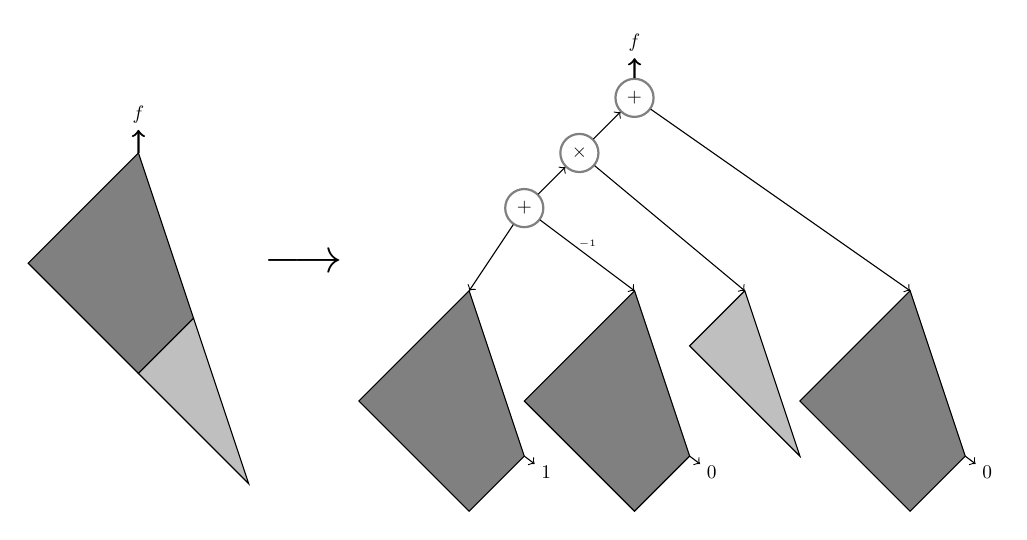
\begin{tikzpicture}[transform shape, scale=0.7]
  \draw[fill=gray] (-10,-2) -- ++(-2,-2) -- ++(2,-2) -- ++(1,1) -- cycle;
  \draw[fill=gray!50] (-9,-5) -- ++(1,-3) -- ++(-2,2) -- cycle;

    \node at (-10,-1.3) {$f$}
    edge[<-,thick] (-10,-2) ;

  
  \node at (-7,-4) {\Huge $\longrightarrow$};
  
  \node (ph) at (-1,0) {$f$};
  \node[gate] (root) at (-1,-1) {$+$}
  edge[thick,->] (ph)
  edge[->] (4,-4.5);
  \node[gate] (m1) at (-2,-2) {$\times$}
  edge[->] (root)
  edge[->] (1,-4.5);
  
  \draw[fill=gray] (4,-4.5) -- ++(-2,-2) -- ++(2,-2) -- ++(1,1) -- cycle;
  \node at  (5.4,-7.8) { $0$}
  edge[<-] (5,-7.5);
  
  \node[gate] (s1) at (-3,-3) {$+$}
  edge[->] (m1)
  edge[->] (-4,-4.5)
  edge[->] node[above] {\tiny $-1$} (-1,-4.5);
  
  \draw[fill=gray!50] (1,-4.5) -- ++(1,-3) -- ++(-2,2) -- cycle;
  
  
  \draw[fill=gray] (-4,-4.5) -- ++(-2,-2) -- ++(2,-2) -- ++(1,1) -- cycle;
  \node at  (-2.6,-7.8) { $1$}
  edge[<-] (-3,-7.5);
  
  \draw[fill=gray] (-1,-4.5) -- ++(-2,-2) -- ++(2,-2) -- ++(1,1) -- cycle;
  \node at  (0.4,-7.8) { $0$}
  edge[<-] (0,-7.5);
\end{tikzpicture}
\end{center}
\caption{Depth reduction for formulas}
\label{fig:formula-depth-red}
\end{figure}

\subsection{Depth reduction for arithmetic circuits}

The key point in the above depth reduction was that for any node $v$, the formulas $\Phi_v$ and $\hat{\Phi}_v(y)$ were disjoint. 
This however is not the case for general arithmetic circuits. 
Thus, it is not clear if we can find a node in the circuit such that the subcircuit under it has size between $s/3$ and $2s/3$. 
However, we do not really need to make the subcircuits have size drop by a constant factor, but any parameter dropping by a constant factor would be fine. 
One parameter that we could work with instead is the \emph{degree}. 


\subsubsection{Applying Brent's reduction with degree}

By \autoref{lem:homogenization}, we may assume that we have a homogeneous circuit $\Phi$ if size $s$ computing a homogeneous $n$-variate polynomial $f$ of degree $d$. 
Using a similar argument as in the proof of \autoref{lem:formula-depth-reduction}, we can find a node $v \in \Phi$ such that $\frac{d}{3} < \deg(v) \leq \frac{2d}{3}$. 
However, we cannot quite write $f$ as $A \cdot \Phi_v + B$ as we are now dealing with a circuit and there could be multiple paths from the root leading to $v$.

Consider the set of all nodes of such intermediate degree as $\mathcal{F}$:
\[
\mathcal{F} = \setdef{v\in \Phi}{\frac{d}{3} < \deg(v)\leq \frac{2d}{3}}
\]
Instead of expressing $f$ using a single $v\in \mathcal{F}$ as in \autoref{lem:formula-depth-reduction}, we shall express $f$ as a function of \emph{all} nodes in $\mathcal{F}$. 

\begin{claim}
If $\mathcal{F} = \inbrace{v_1,\dots, v_s}$, then $f$ may be written as
\begin{equation}\label{eqn:hyafil}
f \spaced{=} \sum_{i,j} A_{ij} \cdot \Phi_{v_i} \Phi_{v_j} \spaced{+} \sum_i B_i \cdot \Phi_{v_i}
\end{equation}
where $\deg(A_{ij}), \deg(B_i) \leq \frac{2d}{3}$ for all $i,j$. 
Moreover, each $A_{ij}$ and $B_i$'s may be computed by an arithmetic circuit of size at most $O(s)$. 
\end{claim}
\begin{proof}
From the circuit $\Phi$, construct the circuit $\Phi'$ that is obtained by removing the incoming edges of every $v_i \in \mathcal{F}$ thereby making these nodes as leaves as well. 
Then, $\Phi'$ computes a polynomial $f'(x_1,\dots x_n, v_1,\dots, v_s)$ satisfying 
\[
f \spaced{=} f'(x_1,\dots, x_n, \Phi_{v_1},\dots, \Phi_{v_s}).
\]
Because of the degree of each $v_i$, we easily obtain that the degree of $f'$ in the $v_i$ variables must be at most $2$, and each coefficient $A_{ij}$ or $B_i$ cannot have degree more than $2d/3$. 
Further, obtaining the $A_{ij}$'s and $B_i$'s from $\Phi'$ is a simple exercise. 
\end{proof}

Since every polynomial appearing in \eqref{eqn:hyafil} is computable by size at most $\poly(s)$ and has degree at most $2d/3$, we may apply induction as earlier. 
Thus,
\begin{eqnarray*}
\mathrm{Depth}(d) & = & \mathrm{Depth}(2d/3) \quad + 2\\
\implies \mathrm{Depth}(d) & = & O(\log d)
\end{eqnarray*}
Unfortunately, the size of the resulting circuit could be as large as $s^{O(\log d)}$. 
This reduction is along the lines of Hyafil~\cite{Hyafil1978}. 

Notice that in this reduction, the final circuit we obtain is in fact an arithmetic formula of size $s^{O(\log d)}$ and depth $O(\log d)$ (assuming that addition gates can have unbounded fan-in; with bounded fan-in addition gates, the depth would be $O(\log d \cdot \log s)$). 
Valiant, Skyum Berkowitz and Rackoff \cite{vsbr83} showed that we can attain a similar depth reduction to $O(\log d)$ depth while keeping the size polynomial. 


\subsubsection{Depth reduction of \cite{vsbr83}}


This section shall be devoted to the proof of the remarkable theorem of Valiant, Skyum, Berkowitz and Rackoff.\footnote{The proof described here follows the structure of a subsequent result \cite{ajmv98}, and not the original proof, although both proofs are quite similar.}


\begin{theorem}[\cite{vsbr83,ajmv98}]\label{thm:vsbr}
  Let $f$ be an $n$-variate degree $d$ polynomial computed by an
  arithmetic circuit $\Phi$ of size $s$. 
Then there is an arithmetic
  circuit $\Phi'$ computing $f$ and has size $s' = \poly(s,n,d)$ and
  depth $O(\log d)$.
\end{theorem}

We may assume without loss of generality that $\Phi$ is a homogeneous
circuit. 
We will also assume that all multiplication gates in $\Phi$
have fan-in at most $2$, and that the degree of the right child of any
multiplication gate is at least as large as the degree of the its left
child. 
Such circuits are known to as \emph{right heavy} circuits. 
For any gate $u$ in $\Phi$, we denote by $[u]$ the polynomial computed at
gate $u$. 
It will also denote a gate label in the new depth reduced
circuit.

We need the following definition of gate quotients.

\begin{definition}\label{defn:gate-quotient}
For any pair of gates $u,v$, the polynomial $[u:v]$ is defined as follows:
\begin{enumerate}
\item If $u$ and $v$ are the same nodes, then $[u:v] = 1$. 
\item If $u$ is a leaf, and $u\neq v$, then $[u:v] = 0$. 
\item If $u = u_1 + u_2$, then $[u:v] = [u_1:v] + [u_2:v]$.
\item If $u = u_1 \times u_2$, then $[u:v] = [u_1] \cdot [u_2 : v]$. \qedhere
\end{enumerate}
\end{definition}

\noindent
It is easy to see that $[u:v]$ is a homogeneous polynomial of degree
$\deg(u) - \deg(v)$. 

\subsection*{Some Intuition}

For an arithmetic formula $\Phi$ with $u$ as root, and any other node
$v$, we can write $\Phi = [u]$ as $A \cdot [v] + B$ for some
polynomials $A$ and $B$. 
We would like to denote $[u:v]$ to denote the
quotient $A$. 
In a circuit things get complicated due to multiple
paths from the $u$ to $v$.

A minimal computation in a circuit is formalized by the notion of a \emph{proof-tree}. 
A proof-tree is a sub-circuit $T$ such that,
\,1. the root is in $T$.
\,2. if a multiplication gate $v$ is in $T$, then so are both its children. 
And,
\,3. if an addition gate $v$ is in $T$, then exactly one child of $v$ is also in $T$.

Every proof-tree computes a monomial, and the polynomial computed by
the circuit is just the sum over all proof-trees. 
The technical issue
in defining the gate quotient stems from the fact that a node $v$
could occur multiple times in a proof-tree, and the number of
occurrences could also vary with different proof-trees. 
To
consistently define the gate quotient, we need to be careful which of
these $v$'s we are referring to. 
We do this by defining the right-most
path in the proof-tree as a canonical path, and replacing the unique
occurrence of $v$ on this canonical path by a leaf labelled $1$ (and
if $v$ does not occur on this path, then this proof-tree does not
contribute to $[u:v]$). 
In fact, it can be seen that
\autoref{defn:gate-quotient} is precisely this notion although
stated algebraically, and this was the perspective used in
\cite{ajmv98}. 
Although it provides more intuition, we
will not use the notion of proof-trees any further to prove
\autoref{thm:vsbr}.

A possible alternate definition is to interpret $u$ as a polynomial in
$v$, and take the first-order partial derivative (as described in
\cite{sy}). 
In the case when $\deg(v) > \deg(u)/2$, this notion
coincides with the above definition of $[u:v]$ (as $v$ cannot occur
more than once in any proof-tree). 
However, some of key properties
(especially \autoref{lem:vsbr-key-lemma} that we shall soon see) are
not true in this setting unless similar degree restrictions are placed
on the pair of nodes. 
While we could reprove \autoref{thm:vsbr} in
this way, we need to be careful about these degree restrictions.

This proof described here can be thought of as a hybrid of
\cite{vsbr83} and \cite{ajmv98}. 
The circuit is built top-down along
the lines of \cite{ajmv98} but using the language of \cite{vsbr83}.


\begin{definition}[Frontier]\label{defn:frontier}
For any parameter $m$, define the \emph{frontier at degree $m$} as
\[
\mathcal{F}_m \quad=\quad \setdef{v}{\deg(v) \geq m\;,\; \deg(v_L), \deg(v_R) < m}
\]
That is, $\mathcal{F}_m$ are the deepest nodes in the circuit that have degree at least $m$. 
\end{definition}

Note that from the above definition, all frontier nodes are
multiplication gates (since we are working with a homogeneous
circuit). 
Also, a frontier forms a maximal anti-chain.

\begin{observation}\label{obs:vsbr-antichain}
  If a node $v$ does not occur in the sub-circuit rooted at $u$, then
  $[u:v] = 0$. 
In particular, if $u, v\in \mathcal{F}_m$ for some $m$, and $u \neq
  v$, then $[u:v]=0$.
\end{observation}

The following is the key lemma for the depth reduction. 

\begin{lemma}\label{lem:vsbr-key-lemma}
Suppose $\Phi$ is a homogeneous, right-heavy circuit. 
Let $m$ be a parameter such that $\deg(u) \geq m$. 
Then,
\begin{equation}\label{eqn:vsbr-for-u}
[u]\spaced{=} \sum_{w\in \mathcal{F}_m} [u:w] \cdot [w]
\end{equation}
Also, if $u,v$ are nodes such that $\deg(u) \geq m > \deg(v)$, then
\begin{equation}\label{eqn:vsbr-for-uv}
[u:v] \spaced{=} \sum_{w\in \mathcal{F}_m} [u:w] [w:v]
\end{equation}
\end{lemma}
\begin{proof}
The proof would be by induction on the depth of $u$.\\

\noindent
1. 
The base case would be when $\deg(u) \geq m$ but all its children have degree less than $m$, that is $u \in \mathcal{F}_m$. 
Such a node $u$ has to be a $\times$ gate. 
Hence,
\begin{eqnarray*}
\sum_{w\in \mathcal{F}_m} [u:w] \cdot [w] &=& [u:u] \cdot [u] \spaced{+}\sum_{\substack{w\in \mathcal{F}_m\\w\neq u}} [u:w] \cdot [w] \spaced{=} [u] \spaced{+} 0\\
\end{eqnarray*}
and
\begin{eqnarray*}
\sum_{w\in \mathcal{F}_m} [u:w] \cdot [w:v] &=& [u:u] \cdot [u:v] \spaced{+}\sum_{\substack{w\in \mathcal{F}_m\\w\neq u}} [u:w] \cdot [w:v] \spaced{=} [u:v] \spaced{+} 0
\end{eqnarray*}
as $[u:w] = 0$ by \autoref{obs:vsbr-antichain}.\\

\noindent
2. 
If $u = u_1 + u_2$,
\begin{eqnarray*}
  [u] &=& [u_1] + [u_2] \\
  &=& \sum_{w\in \mathcal{F}_m} \inparen{[u_1: w]\cdot [w]  + [u_2:w]\cdot [w]}\quad\text{(inductive hypothesis)}\\
  &=& \sum_{w\in \mathcal{F}_m} [u:w] \cdot [w] \quad\text{(\autoref{defn:gate-quotient}.3)}
\end{eqnarray*}
and
\begin{eqnarray*}
  [u:v] &=& [u_1:v] + [u_2:v] \\
  &=& \sum_{w\in \mathcal{F}_m} \inparen{[u_1: w]\cdot [w:v]  + [u_2:w]\cdot [w:v]}\quad\text{(inductive hypothesis)}\\
  &=& \sum_{w\in \mathcal{F}_m} [u:w] \cdot [w:v] \quad\text{(\autoref{defn:gate-quotient}.3)}
\end{eqnarray*}


\noindent
3. 
If $u = u_1 \times u_2$ with $\deg(u_2) \geq m$, 
\begin{eqnarray*}
[u] &=& [u_1] \cdot [u_2]\\
    &=& [u_1] \cdot \inparen{\sum_{w\in \mathcal{F}_m} [u_2:w]\cdot [w]} \quad\text{(inductive hypothesis)}\\
    &=& \sum_{w\in \mathcal{F}_m}([u_1]\cdot [u_2:w]) \cdot [w] = \sum_{w\in \mathcal{F}_m}[u:w] \cdot [w]\quad\text{(\autoref{defn:gate-quotient}.4)}
\end{eqnarray*}
\begin{eqnarray*}
[u:v] &=& [u_1] \cdot [u_2:v]\\
    &=& [u_1] \cdot \inparen{\sum_{w\in \mathcal{F}_m} [u_2:w]\cdot [w:v]} \quad\text{(inductive hypothesis)}\\
    &=& \sum_{w\in \mathcal{F}_m}([u_1]\cdot [u_2:w]) \cdot [w:v] = \sum_{w\in \mathcal{F}_m}[u:w] \cdot [w:v]\quad\text{(\autoref{defn:gate-quotient}.4)}
\end{eqnarray*}

\end{proof}

Now we are ready to write down the depth reduced circuit. 
As mentioned
earlier, the original proof of \cite{vsbr83} follows a bottom-up
approach, but it would be more useful to us to take a top-down
approach (as in \cite{ajmv98}) to obtain some additional structural
properties that we would require.\\

\begin{theorem}[\autoref{thm:vsbr} restated]\label{thm:vsbr-with-structure}
Let $\Phi$ be a homogeneous, right-heavy circuit of size $s$ computing an $n$-variate degree $d$ polynomial. 
Then, there is a circuit $\Phi'$ of size $\poly(s)$ with the following properties:
\begin{enumerate}
\item For every pair of nodes  $u,v\in \Phi$, there are nodes in $\Phi'$ computing $[u]$ and $[u:v]$.
\item For every multiplication gate in $\Phi'$, all its children have at most half its degree. 
\end{enumerate}
\end{theorem}
\begin{proof}
  We shall recursively compute each node $[u]$ and $[u:v]$ from nodes of lower degree. \\

  \noindent
  For any node $u\in \Phi$, let $\mathcal{F}(u) = \mathcal{F}_m$, where
  $m = \deg(u)/2$. 
Thus by \eqref{eqn:vsbr-for-u},
  \begin{eqnarray*}
    [u] & = & \sum_{w\in \mathcal{F}(u)} [u:w] \cdot [w]\\ 
    & = & \sum_{w\in \mathcal{F}(u)} [u:w] \cdot [w_L] \cdot [w_R]
  \end{eqnarray*}
  By our choice of $m$, all the terms on the RHS have degree at most
  $\deg(u)/2$. 
Also, $[u]$ is an addition gate with fan-in $s$ and the
  multiplication gates feeding into it have fan-in $3$.\\
  
  \noindent
  For any pair of nodes $u,v\in \Phi$, let $\mathcal{F}(u,v) =
  \mathcal{F}_m$, where $m = (\deg(u) + \deg(v))/2$. 
By
  \eqref{eqn:vsbr-for-uv},
  \begin{eqnarray*}
    [u:v] & = & \sum_{w\in \mathcal{F}(u,v)} [u:w] \cdot [w:v]\\ 
    & = & \sum_{w\in \mathcal{F}(u,v)} [u:w] \cdot [w_L] \cdot [w_R:v]
  \end{eqnarray*}
  Again by the choice of $m$, the degree of $[u:w]$ and the degree of
  $[w_R:v]$ is at most $(\deg(u) - \deg(v))/2$. 
The degree of $[w_L]$
  however could be as large as $\deg(u) - \deg(v)$. 
Nevertheless, we can
  use the above expansion once more to write it as
  \begin{eqnarray*}
    [u:v] & = & \sum_{w\in \mathcal{F}(u,v)} [u:w] \cdot [w_L] \cdot [w_R:v]\\
    & = & \sum_{w\in \mathcal{F}(u,v)} [u:w] \inparen{\sum_{p \in \mathcal{F}(w_L)} [w_L:p] \cdot [p_L] \cdot [p_R]}\cdot [w_R:v]\\
    & = & \sum_{w\in \mathcal{F}(u,v)}\sum_{p\in \mathcal{F}(w_L)} [u:w] \cdot  [w_L:p] \cdot [p_L] \cdot [p_R]\cdot [w_R:v]
  \end{eqnarray*}
  Now all the terms on the RHS have degree at most $(\deg(u) -
  \deg(v))/2$ as required. 
Also, $[u:v]$ is an addition gate with fan-in
  $s^2$ and the multiplication gates feeding into it have fan-in $5$.\\
  
  Eventually we shall reach a case where $\deg(u)\leq 1$ or $\deg([u:v])
  \leq 1$. 
These are just linear polynomials over $n$ variables and
  shall be explicitly computed in $\Phi'$.

  Starting with the output gate, it is clear how these steps can be
  used to build a depth reduced circuit in a top-down fashion.
\end{proof}

Observe that the proof also shows that all addition gates in $\Phi'$
have fan-in at most $s^2$ and all multiplication gates have fan-in at
most $5$. 
This completes the list of properties we seek from the depth
reduced circuit.


\subsection{Reduction to depth four circuits}

One of the consequence of a depth reduction such as \autoref{thm:vsbr} is that proving lower bounds for general circuits is reduced to the task of proving lower bounds for $O(\log d)$ depth circuits. 

\begin{corollary}\label{cor:vsbr-contra}
If $f$ is an $n$-variate degree $d$ polynomial that requires super-polynomial (in $n$ and $d$) size circuits of $O(\log d)$ depth to compute it, then any general arithmetic circuit computing $f$ must also be of super-polynomial size. 
\end{corollary}

But, optimistically, we would expect that the \emph{right} lower bound must be truly exponential, and not merely super-polynomial. 
Keeping that in mind, a depth reduction even with a slightly super-polynomial blow-up might be useful in this regard. 
This line was first pursued by Agrawal and Vinay \cite{av08}, and the result was subsequently strengthened by Koiran \cite{koiran} and Tavenas~\cite{Tav13}. 

\begin{theorem}[\cite{av08,koiran,Tav13}] \label{thm:av}
Let $f$ be an $n$-variate degree $d$ polynomial computed by a size $s$ arithmetic circuit. 
Then for any $0< t \leq d$, $f$ can be equivalently computed by a homogeneous $\SPSP^{[t]}$ circuit of top fan-in $s^{O(d/t)}$ and size $s^{O(t + d/t)}$. 
\end{theorem}

If we were to optimize the size of the final depth four circuit, then we should choose $t = \sqrt{d}$ to get a $\SPSP^{[t]}$ circuit of size $s^{O(\sqrt{d})}$. 
Note that this implies that if we could prove a lower bound of $n^{\omega(\sqrt{d})}$ for such $\SPSP^{[\sqrt{d}]}$ circuits, then we would have proved a lower bound for general circuits! 
In fact, in the recent past, we have come pretty close to the required threshold and we shall see them in the later chapters. \\

In this section, we shall see a proof of \autoref{thm:av} but this is not the original proof of Tavenas~\cite{Tav13}. 
We shall see an alternate proof by \cite{saptharishivinay14}, which I find more insightful. 

\begin{proofof}{\autoref{thm:av}}
Let $C$ be the $O(\log d)$ depth  circuit computing $f$ obtained from \autoref{thm:vsbr} applied on the size $s$ circuit computing $f$. 
Let $s'$ be the size of $C$. 
If $g$ is a polynomial computed at any intermediate node of $C$, then from the structure of $C$ (~\autoref{thm:vsbr-with-structure}) we have a homogeneous expression
\begin{equation}\label{eqn:vsbr-expansion}
g \spaced{=} \sum_{i=1}^{s'} g_{i1} \cdot g_{i2} \cdot g_{i3} \cdot g_{i4} \cdot g_{i5} 
\end{equation}
where each $g_{ij}$ is computed by a node in $C$ as well, and $\deg(g_{ij}) \leq \deg(g)/2$. 
If we look at \eqref{eqn:vsbr-expansion} for $f$, then the RHS is a $\SPSP^{[d/2]}$ circuit of top fan-in $s'$ computing $f$. 
To obtain a $\SPSP^{[t]}$ circuit eventually, we shall do the following natural process. 
\begin{quote}
  For each summand $g_{i1}\dots g_{ir}$ in the RHS, if the largest degree $g_{ij}$ has degree more than $t$, expand that $g_{ij}$ in-place using \eqref{eqn:vsbr-expansion}. 
  
  Repeat this process until all $g_{ij}$'s on the RHS have degree at most $t$. 
\end{quote}

Note that in each iteration of the above procedure, we increase the top fan-in by a multiplicative factor of $s'$, and what we gain is that some the terms in the RHS would now have smaller degrees. 
If we could show that the in $O(d/t)$  iterations  all terms on the RHS have degree at most $t$, then we would have obtained an $\SPSP^{[t]}$ circuit of top fanin $s'^{O(d/t)}$ computing $f$. \\

To bound the number of iterations, let us count the number of terms of degree more than $t/8$ in each term. 
Note that since we would always maintain homogeneity, the number of terms of degree  $t/8$ or more in any summand  is at most $8d/t$. 
Thus, it suffices to show that each iteration increases the number of terms of degree $t/8$ by at least one. 

Note that in \eqref{eqn:vsbr-expansion}, if $\deg(g) = d'$ then the largest degree term of any summand on the RHS is at least $d'/5$ (since the sum of the degrees of the five terms must add up to $d'$). 
Also, the largest degree term can have degree at most $d'/2$. 
Hence there must be at least $d'/2$ degree contributed by the other four factors in each term. 
This implies that the second largest factor in each summand has degree at least $d'/8$. 
Therefore, as long as we are expanding factors using \eqref{eqn:vsbr-expansion} of degree more than $t/8$, we are guaranteed that each new term has at least one more factor of degree more than $t/8$. 
As argued earlier, we can never have more than $8d/t$ such terms in any summand and this bounds the number of iterations by $8d/t$. 

Thus, when the above procedure stops, we have an $\SPSP^{[t]}$ circuit of top fan-in $s'^{O(8d/t)} = s^{O(d/t)}$. 
Observing that any polynomial of degree $t$ can have at most $n^t$ monomials, we get that the size of the circuit overall is at most $s^{O(t + d/t)}$. 
\end{proofof}

Thus, proving a ``good enough'' top fanin (or size) lower bound for the class of $\SPSP^{[t]}$ circuit would suffice for proving lower bounds for general circuits. 
We would be using this fact quite a lot so we state this explicitly as a corollary. 

\begin{corollary}\label{cor:av}
If $f$ is an $n$-variate degree $d$ polynomial that requires homogeneous $\SPSP^{[t]}$ circuits of top fan-in $n^{\omega(d/t)}$ to compute it, then $f$ requires general arithmetic circuits of size $n^{\omega(1)}$ to compute it. 
\end{corollary}

\begin{exercise}\label{exercise:depth-reduction-prod-depth}
Define the product-depth of any circuit to be the maximum number of multiplication gates encountered on any root-to-leaf path. 

Show that for any polynomial $n$-variate degree $d$ polynomial $f$ that can be computed by a size $s$ arithmetic circuit, there is a circuit $\Phi'$ of size $s^{O(d^{1/\Delta})}$ and product depth $\Delta$ computing $f$. 
\end{exercise}

\subsection*{Reduction to depth three}

There have been some further depth reductions results. 

\begin{theorem}[\cite{gkks13b}] If $f$ is an $n$-variate degree $d$ polynomial in $\Q[\vecx]$ that can be computed by an arithmetic circuit of size $s$, then it can be equivalently computed by a depth three circuit of size $s^{O(\sqrt{d})}$. 
\end{theorem}

We shall defer this theorem to later in the interest of presenting more insight and intuition. 
They would be better placed after we have seen a few of the recent lower bounds for restricted depth four circuits (but those who are impatient can find it in \autoref{sec:depth-3-red}). 
We now proceed to see some lower bounds. 


\subsection{Depth reduction for formulas, again}

In this section we shall revisit \autoref{thm:av} when it is applied to formulas.
Do the resulting depth four circuits have any additional structure when we start from a homogeneous formula?
The alternate proof of Saptharishi and Vinay~\cite{saptharishivinay14} provides some insight into this. 

We would need the following lemma that was present in the survey of Shpilka and Yehudayoff \cite{sy} and also in the result of Hrube\v{s} and Yehudayoff \cite{HY11a} that we shall see a proof of in \autoref{chap:multilinear} as \autoref{lem:mult-logproduct} and \autoref{lem:hom-logproduct}.


\begin{lemma}[\autoref{lem:hom-logproduct} stated without proof]\label{lem:hom-logproduct-restated}
  Let $\Phi$ be a homogeneous formula of size $s$ computing a polynomial $p$ of degree $d$.
Then $p$ can be written as a sum of $(s+1)$ \emph{log-product} polynomials, that is,
\begin{equation}\label{eqn:dred-formula-logproduct}
p \spaced{=} f_1 + \cdots + f_{r}\quad\quad \text{with $r \leq s+1$}
\end{equation}
where for each $i \in [r]$, we have $f_i = f_{i1} \cdots f_{i\ell}$ satisfying
\begin{itemize}
\item each $f_{ij}$ is homogeneous, and $\sum_j \deg(f_{ij}) = d$,
\item $(1 / 3)^j \cdot d \leq \deg(f_{ij}) \leq (2/ 3)^j \cdot d$,
\item $f_{i\ell} = 1$.
\end{itemize}
In particular, each $f_i$ factors into $\Omega(\log d)$ non-trivial factors of geometrically decreasing degrees. 
\end{lemma}

Furthermore, if $\Phi$ was a multilinear formula to begin with, then so is the expression on the RHS.
And if $\Phi$ was set-multilinear, then so is the expression on the RHS.
In other words, it says that a homogeneous formula has a homogeneous depth-$4$ formula of the form $\Sigma^{[s+1]}\Pi^{[\log d]}\Sigma\Pi^{[2d/3]}$.
We can now describe the mild extension of \autoref{thm:av} applied for homogeneous formulas. 

\begin{theorem}[\autoref{thm:av} for homogeneous formulas]\label{thm:av-formulas}
Let $f$ be a homogeneous $n$-variate degree $d$ polynomial computed by a size $s$ homogeneous formula. 
Then for any $0< t \leq d$, $f$ can be equivalently computed by a homogeneous $\Sigma\Pi^{[a]}\Sigma\Pi^{[t]}$ formula of top fan-in $s^{10(d/t)}$ where 
\[
a \geq \frac{1}{10}\pfrac{d}{t} \log t.
\]
\end{theorem}
What this means is that even though the degree of all polynomials computed by the bottom two levels of the $\SPSP$ circuit have degree bounded by $t$, each summand is a product of much more than $d/t$ factors. Another way to view this is that \autoref{thm:av} gives a $\SPSP$ circuit of size $s^{O(d/t)}$ where the maximum bottom degree and \emph{average bottom degree} are both bounded by $O(t)$. Whereas in the above theorem we have maximum bottom degree bounded by $t$ but \emph{average bottom degree} bounded by $(t / \log t)$. 

\begin{proof}The proof is exactly along the lines of \autoref{thm:av}
  but instead of using the $5$-product expression in \eqref{eqn:vsbr-expansion}, we shall use the log-product expression of \eqref{eqn:dred-formula-logproduct}.
The key point again is that in every such summand, there are two factors of degree at least $d/9$.
Therefore, the proof of \autoref{thm:av} proceeds verbatim and the number of iterations is bounded by $9(d/t)$.
This gives the $\SPSP^{[t]}$ formula of size at most $(s+1)^{9(d/t)} \leq s^{10(d/t)}$.
The only thing left to check is that we do indeed have $\Omega((d\log t) / t)$ non-trivial factors in each summand. We leave this as an exercise with a hint. 
\end{proof}

\begin{exercise} Complete the proof of \autoref{thm:av-formulas} by showing that the number of non-trivial factors in any summand of the resulting $\SPSP^{[t]}$ circuit has $\Omega((d\log t)/t)$ non-trivial factors. 

{\bf Hint:} Show that in \eqref{eqn:dred-formula-logproduct}, in any summand, if we only consider the factors of degree at most $t$, the sum of their degrees is at most $2t$. Use that to say each term must involve $\Omega(d/t)$ expansions via \eqref{eqn:dred-formula-logproduct} thus yielding $\Omega((d\log t)/t)$ factors. 
\end{exercise}

This additional structure may be useful in the quest for proving homogeneous formula lower bounds but at the moment it seems unclear. We shall however see one application of this additional structure later in \autoref{chap:tensorrk}. 

%%% Local Variables: 
%%% mode: latex
%%% TeX-master: "fancymain"
%%% End: 


\part{Classical lower bounds}

\include{chap_classicalLBs}

\include{chap_dc}

\include{chap_simpleLBs}

\part{Partial Derivative Spaces}

\chapter{Lower bounds for depth-3 circuits}\label{chap:d3SW}

In this chapter, we shall see the lower bound of Shpilka and Wigderson~\cite{sw2001} for non-homogeneous depth-$3$ circuits over arbitrary fields.
The main theorem of this section would be the following \emph{quadratic} lower bound. 

\begin{theorem}[\cite{sw2001}]\label{thm:SW-SPS-main-thm}
Any $\SPS$ circuit that computes the polynomial $\ESym_d$, for $d = n/100$ must have at least $\Omega(n^2)$ wires. 
\end{theorem}

In fact, $\ESym_d$ can indeed be computed by a $O(n^2)$-sized  $\SPS$ circuit over a characteristic zero field (\autoref{ex:ben-or-trick}) and hence the above result is tight for $\ESym_d$. 
Until recently, this was the best lower bound we knew for the class of general $\Sigma\Pi\Sigma$ circuits but a very recent result of Kayal, Saha and Tavenas~\cite{kst16} has improved this to an almost cubic lower bound (for a different explicit family of polynomials) which we shall see at a later point.
This chapter however shall focus on the proof of the above theorem.

\section{Lower bounds for hom. $\SPS$ circuits \cite{nw1997}}

Let us first consider the following restricted question.
Say we want to compute an $n$-variate degree $d$ polynomial $f$ using a $\SPS$ circuit, but under the restriction that all intermediate computations have degree at most $d$.
The class of such circuits are denoted by $\Sigma\Pi^{[d]}\Sigma$ circuits.
Can we prove lower bounds for this class first?

Indeed, and in fact we have already seen how to in \autoref{chap:simpleLBs}. But it would be good to recall the method again as we would be using this heavily. 

\begin{theorem}[\cite{nw1997}]\label{thm:hom-depth-3-lb-esym}
Any $\Sigma\Pi^{[d]}\Sigma$ circuit that computes $\ESym_d$ must have size $\frac{\binom{n}{d/2}}{2^d}$. 
\end{theorem}
Thus, if $n = 3d$, this gives an exponential lower bound. 

\begin{proof}
For a polynomial $f$, define the \emph{dimension of $k$-th order partial derivatives}, denoted by $\CM{NW}_k(f)$, as follows
\[
\CM{NW}_k(f) \spaced{=} \dim \partial^{=k}(f)
\]
\begin{claim}\label{claim:d3-nw-upperbound}
  If $f = \ell_1 \cdots \ell_d$ where each $\ell_i$ is a linear polynomial, then $\CM{NW}_k(f) \leq \binom{d}{k}$. 
  Thus, if $f = \ell_{11}\cdots \ell_{1d} + \cdots + \ell_{s1}\cdots \ell_{sd}$, then $\CM{NW}_k(f) \leq s \cdot \binom{d}{k}$. 
\end{claim}

\noindent
A fact that we would need here but won't prove is that $\ESym_d$ has large space of partial derivatives. 

\begin{claim}
\[
\CM{NW}_k(\ESym_d) = \min\inparen{\binom{n}{d-k}, \binom{n}{k}}
\]
Hence, for $k = d/2$, we get 
\[
\CM{NW}_k(\ESym_d) = \binom{n}{d/2}.
\]
\end{claim}

\noindent 
The theorem follows directly from these two claims. \qedhere
\end{proof}

\section{Handling \emph{few} high degree gates}

In the last section we saw a way to prove lower bounds for $\SPS$ circuits were the degree of each product of linear forms was bounded by $d$. Suppose we had a $\SPS$ circuit $C$ such that all but say two of the products of linear forms have degree bounded by $d$. That is,
\[
C = C' + T_1 + T_2
\]
where $C' \in \Sigma\Pi^{[d]}\Sigma$ and  $T_1,T_2$ is a product of linear forms of degree possibly larger than $d$. Can we prove lower bounds for such circuits as well? \\

{\bf Key Idea: } Replace some variables by linear functions in other variables to make $T_1$ and $T_2$ equal to zero. \\

Say $T_1$ had one of the linear polynomials as $x_1 + 3x_2 + 5x_3 - 4$, then we shall replace $x_1$ by $- (3x_2 + 5x_3 - 4)$.
The result is that $T_1$ now becomes zero.
What happens to $T_2$?
Note that $T_2$ after this substitution still remains a product of linear polynomials, and its degree cannot increase in this process.
However, it may be the case that $T_2$ was $(x_1 + 3x_2 + 5x_3 - 7)^{2d}$ and under our substitution of $x_1$ this reduces to a constant.
But this is still good because the goal is to eliminate all high degree $T_i$s completely (either by making them zero, or reducing them to constants).
This was the key idea of Shpilka and Wigderson~\cite{sw2001} and we shall formalize this as a lemma.

\begin{lemma}\label{lem:d3-few-affine-projection}
  Let $C = T_1 + \cdots + T_s$ be a $\Sigma\Pi\Sigma$ and suppose $r$ of the $T_i$s have degree greater than $d$.
Then by taking an \emph{affine projection of co-dimension at most $r$}, that is by setting at most $r$ variables to linear functions in the remaining variables, the resulting circuit $C' = T_1' + \cdots T_{s'}'$ is a $\Sigma\Pi^{[d]}\Sigma$ circuit with $s' \leq s$.
\end{lemma}

In order to prove a lower bound for $\Sigma\Pi^{[d]}\Sigma$ circuits, we needed to find a polynomial $f$ for which $\dim \partial^{=k}(f)$ is large.
The strategy to prove lower bounds for $\Sigma\Pi\Sigma$ circuits with $r$ or fewer \emph{high degree} $T_i$s is now clear:
\begin{quote}
  Find a polynomial $g$ such that for every $g'$ that is an \emph{affine projection of co-dimension $r$} on $g$ (that is, obtained from $g$ by setting at most $r$ variables to linear functions in the remaining), we have that $\dim \partial^{=k}(g')$ is large.  
\end{quote}

\section{Shpilka and Wigderson's lower bound for $\Sigma\Pi\Sigma$ circuits}

Shpilka and Wigderson~\cite{sw2001} show that $\ESym_d$ not only has a large $\dim \partial^{=k}$, it also has large $\dim \partial^{=k}$ even after affine projections of co-dimension $d/100$. 

\begin{theorem}[\cite{sw2001}]\label{thm:SW-Esym-robust} Consider the polynomial $\ESym_d$ for any $d < \frac{n}{100}$. If $g$ is an affine projection of $\ESym_d$ of co-dimension $r < \frac{d}{100}$, then
\[
\dim \partial^{=k}(g) \spaced{\geq} \min\inparen{\binom{n-2r}{k},\binom{n-2r}{d-2r -k}}.
\]
Thus, if $k = (d-2r)/2$, then 
\[
\dim \partial^{=k}(g) \geq \binom{n-2r}{(d-2r)/2}.
\]
\end{theorem}

We shall defer the proof of \autoref{thm:SW-Esym-robust} to the end of this section but see why the above theorem implies \autoref{thm:SW-SPS-main-thm}. 

\begin{proof}[Proof of \autoref{thm:SW-SPS-main-thm}]
Consider the polynomial $\ESym_d$ for $d = \frac{n}{100}$. Suppose it is computable by a $\Sigma\Pi\Sigma$ circuit $C = T_1 + \cdots + T_s$ with at most $\frac{d^2}{100}$ wires. Let $r$ be the number of $T_i$s of degree more than $d$. Note that, given the bound on the number of wires, there cannot be more than $\frac{d}{100}$ $T_i$s that have degree more than $d$. Hence, we know that $r \leq \frac{d}{100}$. 

Now that $r \leq \frac{d}{100}$, by \autoref{lem:d3-few-affine-projection}, there is an affine projection $\rho$ of co-dimension at most $r$ such that 
\[
\rho(\ESym_d) \spaced{=} T_1' + \cdots + T_s' \spaced{\in} \Sigma\Pi^{[d]}\Sigma
\]
with $\deg(T_i') \leq d$ and $s \leq \frac{d^2}{100}$. 

But then, on the one hand we know from \autoref{claim:d3-nw-upperbound} that $\CM{NW}_k(\rho(\ESym_d))$ is at most $s \cdot \binom{d}{k}$ but on the other hand \autoref{thm:SW-Esym-robust} states that $\CM{NW}_k(\rho(\ESym_d))$ is \emph{large}. If we set the value of $k$ right ($k=(d-2r)/2$ should work) we get a contradiction to the original assumption that $s < \frac{d^2}{100}$. 

Hence, $s > \frac{d^2}{100} = \Omega(n^2)$ as claimed by the theorem. 
\end{proof}

This entire discussion can be summarized in the following very general remark.

\begin{mdframed}
\begin{remark}\label{rem:meta-SW-lb}
  Suppose we have a measure $\Gamma$ to prove lower bounds for a degree $d$ polynomial computed by a $\Sigma\Pi^{[D]}\Sigma$ circuit. If we can find an explicit polynomial $f$ of degree $d$ with the following properties,
  \begin{itemize}
  \item $\Gamma(f)$ is \emph{large},
  \item even after an affine restriction $\rho$ of co-dimension $r$, we have $\Gamma(\rho(f))$ is \emph{large}
  \end{itemize}
  Then, we can get a $\Omega(Dr)$ lower bound for $f$. 
\end{remark}
\end{mdframed}
What we did above was choose the polynomial $f$ as $\ESym_d$ with $D = d = \Omega(n)$ and using the fact that the partial derivative space remains large even after an affine restriction of co-dimension $r = \Omega(d)$, we get a $\Omega(d^2) = \Omega(n^2)$ lower bound for $\SPS$ circuits.

However, this remark is quite general and in principle, if we could prove a lower bound for say $\Sigma\Pi^{[d^2]}\Sigma$ circuits using some measure, then we could potentially extend this to give a cubic lower bound using the affine projection idea.
In fact, Kayal, Saha and Tavenas \cite{kst16} (which was subsequently strengthened by Balaji, Limaye and Srinivasan \cite{BLS16}) do indeed show an \emph{almost} cubic lower bound using a measure that we shall be discussed later.


\begin{theorem}[\cite{kst16}] There is an explicit $n$-variate poylnomial $f$ of degree $d$ such that any $\SPS$ circuit computing $f$ must require $\Omega\inparen{n^3}{\poly \log(n)}$ size. 
\end{theorem}

Much later in the survey\footnote{This isn't yet finished; will add this shortly}, we shall see the proof of Balaji, Limaye and Srinivasan \cite{BLS16} that, besides being a much simpler and modular proof of \cite{kst16}, also proves the lower bound for a polynomial computed by a depth-$5$ circuit.

\subsection{Rough proof of Theorem~\ref{thm:SW-Esym-robust}}

Let us order the variables as $x_1 \succ x_2 \succ \cdots \succ x_n$.
Say we have an affine projection $\rho$ of co-dimension $r$ that sets the linear polynomials $\set{\ell_1,\ldots, \ell_r}$ to zero. Let $x_{i_j}$ be the \emph{highest} variables participating in each $\ell_j$, that is,
\[
  \ell_j \spaced{=} x_{i_j} - \ell_j'.
\]
Thus, applying this affine restriction is equivalent to replacing each $x_{i_j}$ by $\ell_{j}'$. To get a sense of what this does to $\ESym_d$, let $y_j$ be the \emph{highest variable} participating in $\ell_j'$.

Let us now look at $\ESym_d$, paying attention to the variables $x_{i_j}$s and $y_j$s. We may assume that  $S = \set{x_{i_1},\ldots, x_{i_r}, y_1,\ldots, y_r}$ are all distinct variables (why?).
\begin{eqnarray*}
  \ESym_d(x_1,\ldots, x_n) & = &  x_{i_1}\cdots x_{i_r}\cdot y_1\cdots y_r \cdot \ESym_{d - 2r}(\vecx \setminus S) \spaced{+} \text{other monomials}
\end{eqnarray*}
Replacing each $x_{i_j}$ by $\ell_j'$ introduces higher powers of $y_1,\ldots, y_r$.

\begin{claim}
  If we collect all monomials in $\rho(\ESym_d)$ that are divisible by $y_1^2\cdots y_r^2$, it is precisely
  \[
    y_1^2 \cdots y_r^2 \cdot \ESym_{d-2r}(\vecx \setminus S).
  \]
\end{claim}

\begin{exercise}
Prove this claim. 
\end{exercise}

That is, such monomials can \emph{only} be generated by the first term in the above equation. Now, if we only choose to differentiate by monomials in $\vecx \setminus S$, the remaining monomials do not interfere with the monomials that are divisible by $y_1^2 \cdots y_r^2$. Therefore we get
\[
  \dim \partial^{=k}(\rho(\ESym_d)) \;\geq\; \dim \partial^{=k}\ESym_{d-2r}(\vecx \setminus S) \;=\; \min\inparen{\binom{n-2r}{d-2r-k}, \binom{n-2r}{k}}.\qed
\]

% \section{Revisiting the hom. $\SPS$ lower bound of \cite{nw1997}}

% From \autoref{obs:low-rank-sps-rank}, if $T = \ell_1 \cdots \ell_d$ then for every $0\leq k \leq d$ we have
% \[
% \dim \partial^{=k}(T) \spaced{\leq} \binom{d}{k}. 
% \]
% For a polynomial such as the $\Det_n$, we know that $\partial^{=k}(\Det_n) = \binom{n}{k}^2$. Let us first get a sense of what is the best $k$ to choose for proving lower bounds for $\Sigma\Pi^{[d]}\Sigma$ circuits. We recall some bounds on binomial coefficients from \autoref{chap:binom-estimates}. 

% \begin{proposition*}[\autoref{prop:binom-ub-lb}]For any $n\geq k \geq 0$, 
% \[
% \pfrac{n}{k}^k \spaced{\leq} \binom{n}{k} \spaced{\leq} \pfrac{ne}{k}^k\qedhere
% \]
% \end{proposition*}

% \begin{lemma}[\cite{nw1997}]\label{NW:d3hom-mainlemma} For any $d \geq 0$, any $\Sigma\Pi^{[d]}\Sigma$ circuit computing $\Det_n$ must have size $\exp\inparen{\Omega\pfrac{n^2}{d}}$. 
% \end{lemma}
% \begin{proof}
% As just mentioned, if $C = T_1 + \cdots + T_s$ where each $T_i$ is a product of at most $d$ linear polynomials, then 
% \[
% \dim(\partial^{=k}(C)) \spaced{\leq } s \cdot \binom{d}{k}.
% \]
% On the other hand, 
% \[
% \dim(\partial^{=k}(\Det_n)) \spaced{\geq } \binom{n}{k}^2.
% \]
% Therefore, we get a lower bound of 
% \begin{eqnarray*}
% s & \geq & \frac{\binom{n}{k}^2}{\binom{d}{k}}\\
%   & \geq & \pfrac{n}{k}^{2k} / \pfrac{de}{k}^k \spaced{=} \pfrac{n^2}{e\cdot dk}^k
% \end{eqnarray*}
% Thus, by choosing $k = \pfrac{n^2}{2ed}$, we get a lower bound of $2^k = \exp\inparen{\Omega\pfrac{n^2}{d}}$.
% \end{proof}




% \section{The win-win proof of \cite{sw2001}}

% \begin{proof}[Proof of \autoref{thm:SW-SPS-main-thm}]
%  Say $\Det_n$ is computed by $C = T_1 + \cdots + T_s$ where each $T_i$ is a product of linear forms.
% We will prove by induction that $s\geq \frac{n^4}{100\log n} + 1$. Starting with $C$, we shall modify the circuit to a new circuit $C'$ that computes $\Det_{n-1}$ (up to renaming variables). By induction, we shall assume that 
% \[
% \mathrm{size}(C') \spaced{\geq} \frac{(n-1)^4}{100\log (n-1)}.
% \]

% We shall keep in mind a threshold $d$ that would be set shortly (spoiler: $d= n^2/20\log n)$).
% By \autoref{NW:d3hom-mainlemma} we know that if each $T_i$ is a product of at most $d$ linear polynomials, we have a lower bound of $\exp(\Omega(n^2/d))$. We shall say a variable $x_{ij}$ is \emph{$d$-good} in $C$ if each $T_i$ that depends on $x_{ij}$ has degree at most $d$. \\

% {\bf Case 1:} There is a variable in the first row $x_{1j}$ that is $d$-good. 

% \medskip

% \noindent 
% In this setting, consider the polynomial $C' = C_{(x_{1i} = 1)} - C_{(x_{1i} = 0)}$.
% As far as $\Det_n$ is concerned, this is equivalent to taking the derivative with respect to $x_{ij}$ and hence the polynomial is the corresponding $(n-1)\times (n-1)$ minor.
% The circuit $C'$ on the other hand now is a $\Sigma\Pi^{[d]}\Sigma$ circuit with top fan-in at most $2s$, as all $T_i$s in $C$ that do not depend on $x_{ij}$ would now be eliminated.
% By \autoref{NW:d3hom-mainlemma}, this implies that $2s > \exp(\Omega((n-1)^2/d))$ which is certainly bigger than $(n^4 / \log n)$ if $d = n^2/20\log n$.\\

% {\bf Case 2:} There is \emph{no} variable in the first row that is $d$-good. 

% \medskip

% \noindent 
% We know that the variable $x_{12}$ is not $d$-good.
% This means that there is some $T_i$ of degree more than $d$ which has a factor of the form $(x_{12} - \ell)$.
% We shall now set $x_{12} = \ell$ in $C$ and this eliminates the gate $T_i$ altogether and thereby reducing the size by at least $d$ wires. 

% Now move on to $x_{13}$. It is possible now that after eliminating $T_i$ in the previous step, we may now have $x_{13}$ to be $d$-good. Then we reduce to Case 1 and we are done. Otherwise, there is some $T_j$ of degree more than $d$ with a factor of the form $(x_{13} - \ell')$. Once again, we set $x_{13} = \ell'$ to eliminate $T_j$ and thereby reduce the size of the circuit by $d$. \\

% Repeating this process for $\set{x_{12}, \ldots, x_{1n}}$, we either reach Case 1 (in which case we are done), or we have thereby reduced the circuit by at least $d(n-1)$ wires. So far, we have only messed with the variables $\set{x_{12},\ldots, x_{1n}}$ but this is not an issue because we can further set $x_{11} = 1$ and $x_{21} = x_{31} = \cdots = x_{n1} = 0$. Therefore, the polynomial thus computed has to be the minor with respect to $x_{11}$ which is just $\Det_{n-1}$ up to renaming variables. But then,
% \[
% \mathrm{size}(C) \spaced{\geq} \mathrm{size}(C') \;+\; \pfrac{(n-1)^2 n^2}{20\log n}
% \]
% Hence, it follows by induction that $\mathrm{size}(C) \geq \pfrac{n^4}{100\log n} + 1$.
% \end{proof}


%%% Local Variables: 
%%% mode: latex
%%% TeX-master: "fancymain"
%%% End: 


%% Proof of Balaji-Limaye-Srinivasan

\include{chap_GK}

\part[Multilinear and non-commutative models]{Multilinear and non-commutative models}

\include{chap_PDM}

\chapter{Hardness amplification for non-commutative circuits}
\label{chap:nc-hardness-amp}

In \autoref{chap:evalDim}, we saw exponential lower bounds for the non-commutative formulas and ABPs. As mentioned earlier, in the commutative world, this would have immediately yielded lower bounds for circuits as well due to the depth reduction results (\autoref{thm:vsbr}). However this does not happen in the non-commutative world, and proving lower bounds for non-commutative circuits has remained elusive.

In this chapter, we shall see a beautiful result of Carmasino, Impagliazzo, Mihajlin and Lovett~\cite{CILM18} that show that even mildly super-linear lower bounds for a family of non-commutative polynomials can be \emph{amplified} to obtain much stronger lower bounds.

\begin{theorem}[\cite{CILM18}] \label{thm:CILM18-mainthm}
  Suppose there is some $\epsilon > 0$ for which we have an explicit family of non-commuting polynomials $\set{f_n}$ (with $f_n$ being an $n$-variate non-commuting polynomial of degree $\poly(n)$) such that $f_n$ requires non-commutative circuits of size $n^{(\omega/2) + \epsilon}$.

  Then, for every $c \geq 1$, there is an explicit family $\set{g_n}$ (with $g_n$ being an $n$-variate polynomial of degree $\poly(n)$) that requires non-commutative circuits of size $n^c$. 
\end{theorem}

In fact, the conclusion can be strengthened if the initial polynomial family $\set{f_n}$ is a constant degree family.

\begin{theorem}[\cite{CILM18}] \label{thm:CILM18-mainthm-constdeg}
  Suppose there is some $\epsilon > 0$ for which we have an explicit family of non-commuting \emph{constant degree} polynomials $\set{f_n}$ (with $f_n$ being an $n$-variate non-commuting polynomial of degree $d$, which is a constant) such that $f_n$ requires non-commutative circuits of size $n^{(\omega/2) + \epsilon}$.

  Then, for some $\delta \geq 0$, there is an explicit family $\set{g_n}$ (with $g_n$ being an $n$-variate polynomial of degree $\poly(n)$) that requires non-commutative circuits of size $\exp(n^{\delta})$. 
\end{theorem}

In both the above theorems, $\omega$ refers to the exponent of matrix multiplication. For simplicity, we shall just work with this being replaced by $3$. Hence, the above theorems say that if we can get lower bounds of $n^{1.5 + \epsilon}$, then this can be amplified.

\section{Intuition}

Both these theorems go via a clever \emph{hardness-preserving variable reduction}. Formally, we will start with a polynomial $f(x_1,\ldots, x_n) \in \F\inangle{x_1,\ldots, x_n}$ and transform this to a polynomial $g(y_1,\ldots, y_m) \in \F\inangle{y_1,\ldots, y_m}$  where $m \ll n$. This transformation would be obtained by replacing each $x_i$ by some $h_i(y_1,\ldots, y_m)$ for some relatively simple $h_i$'s (in fact, they will just be monomials).

Clearly, if $f$ has a small circuit, then so does $g$ (since each of the $h_i$'s are simple). The key point would be that a rough converse also would hold. That is, if someone provided a size $s$ non-commutative circuit for $g$, then there is a circuit of size $s'$ (which is not-much-larger-than $s$) that computes $f$. As a contrapositive, if $f$ \emph{cannot} be computed by circuits of size $s$, then $g$ \emph{cannot} be computed by circuits of size $s'$. Why is this a hardness amplification? Notice that $m \ll n$; hence $s'$ as a function of $m$ could be way larger than $s$ as a function of $n$.

The proofs of both the theorems essentially repeat the above transformation as many times as possible. In the general case, we can repeat this any constantly many times and hence this would eventually yield \autoref{thm:CILM18-mainthm}. In the setting when the polynomial family has constant degree, we can repeat this more times and that yields \autoref{thm:CILM18-mainthm-constdeg}.

We will see the details in the rest of the chapter. 

\section{The hardness-preserving variable reduction}

Suppose $f \in \F\inangle{x_1,\ldots, x_n}$ is a polynomial of degree $d$. Let $m = \ceil{n^{1/3}}$. To each of the variables $x_i$, we shall assign a unique non-commutative monomial $y_{i_1}y_{i_2}y_{i_3}$. Define the polynomial $g$ obtained from $f$ via by substituting the associated monomial for $x_i$:
\[
\Amp_3(f) :=  g(y_1,\dots, y_m) := f(y_{1_1}y_{1_2}y_{1_3}, \ldots, y_{n_1}y_{n_2}y_{n_3})
\]
Clearly, $g$ is an $m$-variate non-commutative polynomial with  $\deg g \leq 3 d$. 

\begin{lemma}[Hardness-preserving reduction]\label{lem:cilm-mainlemma}
Let $f$ be an $n$-variate non-commutative polynomial. Suppose there is a non-commutative circuit of size at most $s$ that computes $\Amp_3(f)$. Then, there is a non-commutative circuit of size at most $s' = C \cdot s \cdot n^{\omega/3}$ for a universal constant $C$. 
\end{lemma}
We shall assume the above lemma for now and finish the proofs of \autoref{thm:CILM18-mainthm} and \autoref{thm:CILM18-mainthm-constdeg}. We shall define the following operator which applies this amplification multiple times. 
\[
  \Amp_3^{(k)}(f) := \underbrace{\Amp_3 \circ \Amp_3 \circ \cdots \circ \Amp_3}_{\text{$k$ times}} (f).\]
\begin{corollary}[Iterative hardness-preserving reduction]\label{cor:cilm-maincorr}
  Let $f$ be an $n$-variate non-commutative polynomial, of degree $d$, with $n = m^{3^k}$ for some positive integers $m$ and $k$. Let $g(y_1,\ldots, y_m) = \Amp_3^{(k)}(f)$, an $m$-variate non-commutative polynomial of degree $3^k d$. If $g$ can be computed by a circuit of size $s$, then $f$ can be computed by a circuit of size at most $s \cdot n^{\omega/2}\cdot C^k$ where $C$ is the universal constant in \autoref{lem:cilm-mainlemma}
\end{corollary}
\begin{proof}\belowdisplayskip=-12pt
  By repeated applications of \autoref{lem:cilm-mainlemma} yields that $f$ can be computed by a circuit of size at most
  \begin{align*}
    s' & = s \cdot C^k \cdot \inparen{m^{\omega} \cdot  m^{3\omega}\cdots m^{3^{k-1}\omega}}\\
       & = s \cdot C^k \cdot m^{\omega  \cdot (3^{k} - 1)/(3 - 1)}\\
       & \leq  s \cdot C^k \cdot m^{(\omega/2) \cdot 3^k} = s \cdot C^k \cdot n^{\omega/2}.
  \end{align*}
\end{proof}

\begin{proof}[Proof of \autoref{thm:CILM18-mainthm} and \autoref{thm:CILM18-mainthm-constdeg}]
  Let $g = \Amp_3^{(k)}(f)$ for a $k$ that shall be fixed shortly. If $n = m^{3^k}$ of degree $d$, then $g$ is an $m$-variate polynomial of degree $3^k \cdot d$. \autoref{cor:cilm-maincorr} states that if $f$ requires circuits of size $\Omega(n^{(\omega/2) + \epsilon})$ then $g(y_1,\ldots, y_m)$ requires circuits of size $C^k \cdot n^\epsilon$.

  \begin{itemize}
  \item (Proof of \autoref{thm:CILM18-mainthm}) Set $k$ large enough constant so that $3^k \cdot \epsilon > c$. Then $\deg(g) = 3^k d = \poly(n) = \poly(m)$ as $k$ is a constant. Also, $g$ requires circuits of size $\Omega(n^\epsilon) = \Omega(m^c)$ by the choice of $k$.

  \item (Proof of \autoref{thm:CILM18-mainthm-constdeg}) Pick the smallest $k$ such that $3^k \cdot k > \log n$; let $m = n^{1/3^k}$ and $g = \Amp_3^{(k)}(f)$.
Note that for this choice of $k$, we have $k > \log m$. 
    With this choice of $k$ and since $d = \deg(f)$ is a constant, we have
    \[
      \deg(g) = 3^k \cdot d \approx 3^{(\log n) / 3^k} \cdot d = 3^{\log m} \cdot d = \poly(m).
    \]
    Also, $g$ requires circuits of size at least
    \[
      C^k n^\epsilon = m^{3^k \cdot \epsilon} C^k \approx m^{3^k \cdot \epsilon + \log C}= \Omega(\exp(m^\delta))
    \]
    for some $\delta > 0$. \qedhere
  \end{itemize}
\end{proof}

\noindent
In the rest of the chapter we shall see how to prove \autoref{lem:cilm-mainlemma}.

\section{Proof of the main lemma}

We are provided a circuit of size $s$ that computes $\Amp_3(f)$ and we want to use that to find a circuit for $f$. Basically, what we need to do is undo this monomial transformation.

Intuitively, we want to say that there shouldn't be a circuit much better than actually computing $f$ and doing this transformation. Of course, given \emph{such} a circuit for $\Amp_3(f)$, we can just pull out a circuit for $f$. The main idea is that given \emph{any} circuit for $g$, we can always structure the circuit in such a way that it really does look like a circuit computing $f$ and then doing the monomial substitution.

We will first perform a \emph{partial homogenisation} operation, very similar to \autoref{lem:homogenization} but much weaker. This would be the first step towards at least ensuring that each gate computes a polynomial of degree divisible by $3$. 

\begin{definition}[A $(\bmod{3})$-homogeneous circuit] A circuit $C$ is said to be $(\bmod{3})$-homogeneous if every gate is labelled by a pair $(i,j) \in \set{1,2,3}^2$ satisfying the following conditions: 
  \begin{itemize}
  \item All leaves will be labelled by some $(i,j)$ such that $j = i+1 \bmod 3$ if it is a variable, and by some $(i,i)$ if the leaf is a constant.
  \item If $g$ is a $+$ gate with label $(i,j)$, then all its children also have label $(i,j)$.
  \item If $g = g_1 \times g_2$ with label $(i,j)$ then there must be some $k \in \set{0,1,2}$ such that $g_1$ has label $(i,k)$ and $g_2$ has label $(k,j)$. \qedhere
  \end{itemize}
\end{definition}

Intuitively, each gate's label of $(i,j)$ says that its contribution will always be from a position that is $i \bmod 3$ and until $j\bmod 3$. We leave the proof of the following observation as an easy exercise. 

\begin{observation}
  Any non-commutative polynomial that can be computed by a non-commutative circuit of size $s$ can be equivalently computed by a $(\bmod{3})$-homogeneous non-commutative circuit of size at most $9s$.  
\end{observation}

Let us see what would happen if we started with the trivial circuit for $\Amp_3(f)$ obtained from a circuit for $f$ and applying the monomial substitution. The resulting circuit is already $(\bmod{3})$-homogeneous, and \emph{every} gate has label $(1,1)$ (and we are thinking of leaves as now being monomials; they also have label $(1,1)$ then). This is the state we want to get to from an arbitrary circuit. The partial homogenisation is one step towards it but there are all kinds of labels for the gates and we want to fix that.

The beautiful idea of Carmosino et al \cite{CILM18} is to replace each gate of the circuit by a $m\times m$ matrix of gates, such that each entry of this matrix would have label $(1,1)$. We then want to simulate all additions and multiplications as matrix multiplications. We will need to build some notation. 

\begin{definition}[Division operators]
  For a polynomial $f \in \F\inangle{y_1,\ldots, y_m}$ and a variable $y \in \set{y_1,\ldots, y_m}$, we shall define the left and right division operators as
  \begin{align*}
    [y^{-1}] f & = \sum_{\substack{\vecw\in \set{y_1,\ldots, y_m}^*\\ \vecw = y \vecw'}} \coeff_\vecw(f) \cdot \vecw'\\
     f [y^{-1}] & = \sum_{\substack{\vecw\in \set{y_1,\ldots, y_m}^*\\ \vecw = \vecw' y}} \coeff_\vecw(f) \cdot \vecw'
  \end{align*}
  In words, $[y^{-1}] f$ divides from the left by $y$ (and monomials that do not begin with $y$ are zeroed out) and $f [y^{-1}]$ divides from the right. 
\end{definition}

We now define an operator that maps every labelled gate of the circuit to a matrix of polynomials each of whose entries are $(\bmod{3})$-homogeneous. We'll call it the \emph{glacial} operator after the following sentence in \cite{CILM18}:
\begin{quote}
  ``This process is like a glacial movement during the ice age. An operator slides over the circuit and then disappears, drastically changing the landscape behind it.''
\end{quote}

\begin{definition}[The \emph{glacial} operator]
  Let $g$ be a gate in a $(\bmod{3})$-homogeneous non-commutative circuit $C$ with label $(a,b)$. Let $g$ also denote the polynomial computed by the gate.

The operator $\Phi(g)$ returns an $m\times m$ matrix of polynomials whose $(i,j)$-th entry is given by the $(a,b)$-th entry of the following matrix:
\begin{align*}
  \insquare{
  \begin{array}{ccc}
    g & g\insquare{y_j^{-1}} & g y_j\\
    y_i g & y_i g\insquare{y_j^{-1}} & y_i gy_j\\
    \insquare{y_i^{-1}} g & \insquare{y_i^{-1}} g\insquare{y_j^{-1}} & \insquare{y_i^{-1}} g\insquare{y_j^{-1}}\\
  \end{array}
  }.
\end{align*}
\end{definition}
What the above definition does is best described in plain words and a few examples. If $g$ is labelled $(1,1)$, then basically $g$ is both \emph{start-aligned} and \emph{end-aligned} and the matrix $\Phi(g)$ would just have $g$ in every entry. If $g$ is labelled $(2,2)$, then $g$ ``needs one symbol on the left to be added'' to become \emph{start-aligned} and ``needs one symbol on the right to be removed'' to become \emph{end-aligned}. The $(i,j)$-th entry of $\Phi(g)$ then corresponds to $y_i g [y_j^{-1}]$, which \emph{aligns} $g$ by adding $y_i$ on the left and removing $y_j$ on the right. 

\begin{observation}\label{obs:cilm-glacial-movement}
  Let $C$ be a $(\bmod{3})$-homogenised circuit of size $s$. Suppose $g$ is some internal gate in $g$.
  \begin{itemize}
  \item If $g = g_1 + g_2$, then $\Phi(g) = \Phi(g_1) + \Phi(g_2)$ (matrix addition).
  \item If $g = g_1 \times g_2$, then $\Phi(g) = \Phi(g_1) \times \Phi(g_2)$ (matrix multiplication). 
  \end{itemize}
\end{observation}

The proof of the above observation is a simple exercise and is left to the reader. Thus, all we need to do for now is replace every gate $g$ of $C$ by the entries of $\Phi(g)$, all addition and multiplication gates by matrix addition and matrix multiplication gates, and we would have obtained our $(\bmod{3})$-homogeneous circuit with each gate labelled with $(1,1)$!

We start with the leaves of $C$ which were computing variables. For any leaf $\ell$, observe that $\Phi(\ell)$ would be an $m\times m$ matrix, each of whose entries is a monomial of degree exactly $3$ or a constant. Thus, we can first  compute $\Phi(\ell)$ for all the leaves $\ell$. If $g = g_1 \circledast g_2$ is some internal gate for which we need to compute $\Phi(g)$, and we have computed $\Phi(g_1)$ and $\Phi(g_2)$, then we can compute the entries of $\Phi(g)$ by a suitable matrix addition/multiplication via \autoref{obs:cilm-glacial-movement}.

And finally, each matrix addition and matrix multiplication of $m\times m$ matrices can be simulated\footnote{technically, it should be $O(m^{\omega + \epsilon})$ for every $\epsilon > 0$... but meh.} by $O(m^\omega)$ usual additions and multiplications. Let us summarize this discussion as a lemma. 

\begin{lemmawp}[Alignment lemma]
  Suppose $f \in \F\inangle{y_1,\ldots, y_m}$ is a polynomial such that every monomial of $f$ has degree divisible by $3$ and computable by a non-commutative circuit $C$ of size $s$. Then, there is a $(\bmod{3})$-homogeneous circuit $C'$, each of whose gates/leaves are labelled by $(1,1)$, of size at most $O(s \cdot m^{\omega})$
\end{lemmawp}

\noindent
\autoref{lem:cilm-mainlemma} is a direct corollary of the above lemma as $m = n^{1/3}$ and this completes the proof of the hardness amplification for non-commtuative circuits. 

\vskip 1em


\begin{exercise}
  The main monomial transformation  was replacing the $n$ variables by degree $3$ monomials in $n^{1/3}$ variables. Naturally, one can choose any $r$ and replace each of the $n$ variables by degree $r$ monomials in $n^{1/r}$ variables. How would these bounds change for an arbitrary $r$? 
\end{exercise}

%%% Local Variables:
%%% mode: latex
%%% TeX-master: "fancymain"
%%% End:


\chapter{Lower bounds for multilinear models}\label{chap:multilinear}

Most of the polynomials that are studied usually, like those described in \autoref{chap:notation}, are multilinear. 
A natural question is whether or not multilinear polynomials can be computed in a ``multilinear fashion''. 
This is formalized by what the model of multilinear circuits, in a way analogous to homogeneous circuits. 

\begin{definition}[Multilinear circuits]
A circuit $C$ is said to be \emph{multilinear} if every gate of the circuit computes a multilinear polynomial. 
A circuit is said to be \emph{syntactically multilinear} if for any $g = g_1 \times g_2$, there is no variable that has a path to both $g_1$ and $g_2$. 
\end{definition}

Note that syntactic multilinearity of course implies multilinearity as the definition forces all gates to compute multilinear polynomials. 
However, we could have a setting where there is a gate $g = g_1 \times g_2$ where some variable $x$ has a path to both $g_1$ and $g_2$ but it so turns out that $g_1$ is independent of $x$ due to other cancellations. 
However, for arithmetic formulas, the two notions are equivalent. 

\begin{exercise}
Given any arithmetic formula $\Phi$ that is multilinear, show that it can be converted to a formula $\Phi'$ of size $\poly(\Phi)$ that is syntactically multilinear. 

\noindent
{\bf (Imp.)} Why does the same not work for multilinear circuits? 
\end{exercise}

This section shall deal mainly with multilinear formulas so we may assume without loss of generality that they are syntactically multilinear. 
Raz \cite{raz2004} showed that multilinear formulas computing the $\Det_n$ or $\Perm_n$ must be of size $n^{\Omega(\log n)}$. 
The complexity measure used by Raz also led to exponential lower bounds for constant depth multilinear circuits \cite{raz-yehudayoff} and super-linear lower bounds for syntactic multilinear circuits \cite{RSY08}. 
\Hrubes and Yehudayoff~\cite{HY11a} then showed a super-polynomial lower bound \emph{homogeneous} multilinear formulas computing the elementary symmetric polynomial.

Although the lower bound of \Hrubes and Yehudayoff was subsequent to the results of Raz and Yehudayoff~\cite{raz2004,raz-yehudayoff}, we shall see their lower bound first which uses a suprisingly simple complexity measure. For the non-homogeneous setting, the complexity measure used here would also be the \emph{rank of the partial derivative matrix} from \autoref{chap:evalDim}. We shall start off with a structural result whenever we are dealing with formulas, which builds on the depth reduction for formulas \autoref{lem:formula-depth-reduction}. 

\section{Log-product representations for formulas}

The following structural lemma shows that any multilinear formula can be converted in to a small sum of \emph{log-product} polynomials. 
The techniques of the following lemma can also be used in other settings with minor modifications, and we shall encounter a different version of this lemma later as well.
These normal forms is from the survey of Shpilka and Yehudayoff~\cite{sy}, and also from the result of \Hrubes and Yehudayoff~\cite{HY11a}. 

\begin{definition}\label{defn:mult-logproduct}
  A multilinear polynomial $f\in \F[X]$ is called a \emph{multilinear log-product} polynomial if $f = g_1\dots g_t$ and there exists a partition of variables $X = X_1 \sqcup \dots \sqcup X_t$ such that
  \begin{itemize}
  \item $g_i \in \F[X_i]$ for all $i \in [t]$.
  \item $\pfrac{1}{3}^i |X| \leq |X_i| \leq \pfrac{2}{3}^i |X|$ for all
    $i$, and $|X_t| = 1$.
  \end{itemize}
\end{definition}

\begin{lemma}\label{lem:mult-logproduct}
  Let $\Phi$ be a multilinear formula of size $s$ computing a polynomial $p$. 
Then $p$ can be written as a sum of $(s+1)$ log-product multivariate polynomials.
\end{lemma}
\begin{proof}
  Similar to \autoref{lem:formula-depth-reduction}, let $v$ be a node in $\Phi$ such that set of variables $X_v$ that it depends on satisfies $\frac{|X|}{3} \leq \abs{X_v} \leq \frac{2|X|}{3}$. 
If $\Phi_v$ is the polynomial computed at this node, then $f$ can be written as
  $$
  f \spaced{=} \Phi_v \cdot g_1 + \Phi_{v=0} \quad\text{for some $g_1 \in \F[X\setminus X_v]$}.
  $$
  where $\Phi_{v=0}$ is the formula obtained by replacing the node $v$ by zero. 
Note that the subtree at the node $v$ is completely disjoint from $\Phi_{v=0}$. 
Hence the sum of the sizes of $\Phi_v$ and $\Phi_{v=0}$ is at most $s$. 
Hence, $g_1 \in \F[X\setminus X_v]$ and $\frac{|X|}{3} \leq \abs{X \setminus X_v} \leq \frac{2|X|}{3}$. 
Inducting on the formulas $\Phi_v$ and $\Phi_{v=0}$ gives the lemma.
\end{proof}

There are many variants of this formula depending on how you pick the node $v$ in the proof above.
Here is another variant that find a node $v$ based on \emph{degree} rather than the number of variables that it depends on.
We state it here without proof but it follows exactly as in the lines of \autoref{lem:mult-logproduct}.

\begin{lemma}\label{lem:hom-logproduct}
  Let $\Phi$ be a homogeneous formula of size $s$ computing a polynomial $p$ of degree $d$.
Then $p$ can be written as a sum of $(s+1)$ \emph{log-product} polynomials, that is,
\[
p \spaced{=} f_1 + \cdots + f_{r}\quad\quad \text{with $r \leq s+1$}
\]
where for each $i \in [r]$, we have $f_i = f_{i1} \cdots f_{i\ell}$ satisfying
\begin{itemize}
\item each $f_{ij}$ is homogeneous,
\item $(1 / 3)^j \cdot d \leq \deg(f_{ij}) \leq (2/ 3)^j \cdot d$,
\item $f_{i\ell} = 1$.
\end{itemize}
In particular, each $f_i$ factors into $\Omega(\log d)$ non-trivial factors of geometrically decreasing degrees. 

Furthermore, if $\Phi$ was a multilinear formula to begin with, then so is the expression on the RHS. 
\end{lemma}


We shall see yet another variant of this trick later in this chapter but we have enough for now to prove the lower bound of \Hrubes and Yehudayoff \cite{HY11a}. 

\section{Lower bounds for homogeneous multilinear formulas}

The main theorem of this section would be the following.

\begin{theorem}[\cite{HY11a}]\label{thm:Hrubes-Yehudayoff}
Any homogeneous multilinear formula that computes the polynomial $\ESym_d$, for $d \leq n/2$, must have size $d^{\Omega(\log d)}$. 
\end{theorem}

The complexity measure used here would be ridiculously simple --- just the number of monomials!
Surprisingly, this is enough to prove the lower bound for homogeneous multilinear formulas. Before we get into the proof, we would need the following approximation for the binomial coefficient. This follows from Stirling's approximation of $n!$. 

\begin{lemma}[Stirling's approximation of $\binom{n}{k}$]\label{lem:stirling-binom} For $n \geq 3k/2$, the following 
\[
\pfrac{1}{3\sqrt{k}} \cdot \pfrac{n^n}{k^k \cdot (n-k)^{n-k}} \spaced{\leq} \binom{n}{k} \spaced{\leq} \pfrac{1}{\sqrt{k}} \cdot \pfrac{n^n}{k^k \cdot (n-k)^{n-k}}
\]
\end{lemma}

\begin{proofof}{\autoref{thm:Hrubes-Yehudayoff}}
If there is a size $s$ homogeneous multilinear formula computing $\ESym_d$, then by \autoref{lem:hom-logproduct} we have an expression of the form
\[
\ESym_d \spaced{=} \sum_{i=1}^{s+1} f_{i1} \cdots f_{i\ell}
\]
with $\ell = \Omega(\log d)$.
We shall show that each multilinear term of the form $f_{i1} \cdots f_{i\ell}$, with geometrically decreasing degrees, can contribute at most $d^{-\Omega(\log d)} \cdot \binom{n}{d}$ monomials.
This would immediately imply that $s = d^{\Omega(\log d)}$. \\


Consider a term of the form $f_1 \cdots f_\ell$. Since the degrees drop geometrically, we may assume without loss of generality that $\ell = \Omega(\log d)$ and $\deg(f_i) \geq \sqrt{d}$ (by just multiplying all polynomials of smaller degree together). This is a homogeneous multilinear expression so let $\deg(f_i) = d_i$ and let $f_i$ depend on the variables $X_i$. If $n_i = \abs{X_i}$, then each $f_i$ has at most $\binom{n_i}{d_i}$ monomials. Hence, the total number of monomials from this term is at most
\[
\binom{n_1}{d_1} \cdots \binom{n_\ell}{d_\ell}.
\]
All that's left to do is show that this is significantly smaller than $\binom{n}{d}$. 

\begin{lemma}[\cite{HY11a}]\label{lem:HY-prod-binom}
Let $n\geq 2d$. For any set of non-negative integers satisfying $n_1 + \cdots + n_\ell = n$ and $d_1 + \cdots + d_\ell = d$, we have
\[
\binom{n_1}{d_1} \cdots \binom{n_\ell}{d_\ell} \spaced{\leq} 3 \sqrt{\frac{d}{d_1 \cdots d_\ell}} \cdot \binom{n}{d}
\]
\end{lemma}
The theorem immediately follows from this lemma as each $d_i \geq \sqrt{d}$ and there are $\Omega(\log d)$ of them. 

Before we prove this theorem, let us quickly look at the simpler case when $d = n/2$. In that case, $\binom{n}{d} \approx 2^n / \sqrt{n}$ and the LHS is clearly upper bounded as
\[
\binom{n_1}{d_1} \cdots \binom{n_\ell}{d_\ell} \spaced{\leq} \frac{2^{n_1+ \cdots + n_\ell}}{\sqrt{n_1 \cdots n_\ell}}
\]
giving us a similar bound. The case of general $d$ requires a bit more work but is quite natural (once you know it is true). 

\begin{myproof}{\autoref{lem:HY-prod-binom}}[of \autoref{lem:HY-prod-binom}]
Without loss of generality, we may assume that $n_i \geq 2d_i$ for all $i$. We are trying to understand the following distribution:
\begin{quote}
  If we pick $d$ elements out of $n$ elements, what's the probability that we pick $d_1$ elements from the first $n_1$, and $d_2$ from the next $n_2$ ... etc. 
\end{quote}
The first step is to ask, for fixed values of $n_1, \ldots, n_\ell$, what values of $d_1, \ldots, d_\ell$ maximize this probability. Intuitively, each $d_i$ ought to be proportional to $n_i$ as that is what we would get in expectation. In the perfect regime where $n = \alpha \cdot  d$ and  $n_i = \alpha \cdot d_i$ for each $i \in [\ell]$, we can now use the approximation from \autoref{lem:stirling-binom} to get
\begin{eqnarray*}
\binom{n}{d} & \geq  &  \pfrac{1}{3\sqrt{d}} \cdot \pfrac{n^n}{d^d \cdot (n-d)^{n-d}}\\
 & = & \pfrac{1}{3\sqrt{d}} \cdot \pfrac{d^n \cdot \alpha^n}{d^d \cdot d^{n-d} \cdot (\alpha - 1)^{n-d}}\\
 & = & \pfrac{1}{3\sqrt{d}} \cdot \pfrac{\alpha^n}{(\alpha - 1)^{n-d}}\\
\text{and} \quad\binom{n_i}{d_i} & \leq  &  \pfrac{1}{\sqrt{d_i}} \pfrac{\alpha^{n_i}}{(\alpha - 1)^{n_i-d_i}}\\
\implies \binom{n_1}{d_1} \cdots \binom{n_\ell}{d_\ell}  & \leq & 3 \sqrt{\frac{d}{d_1 \cdots d_\ell}} \cdot \binom{n}{d}
\end{eqnarray*}

To complete the proof, we just have to show that $\binom{n_1}{d_1} \cdots \binom{n_\ell}{d_\ell}$ is maximized when $n_i/d_i \approx n/d$.
To do this, let us consider a term $\binom{n_1}{d_1} \cdot \binom{n_2}{d_2}$ with $d_1/n_1 \gg d_2/n_2$ and show that $\binom{n_1}{d_1 - 1} \cdot \binom{n_2}{d_2 + 1}$ is larger.
This is easy to see because
\begin{eqnarray*}
\frac{\binom{n_1}{d_1 - 1} \cdot \binom{n_2}{d_2 + 1}}{\binom{n_1}{d_1} \cdot \binom{n_2}{d_2}} & = & \frac{d_1 \cdot (n_2 - d_2)}{(n_1 - d_1 + 1) \cdot (d_2 + 1)}\\
 & = & \frac{\pfrac{n_2 + 1}{d_2 + 1} - 1 }{\pfrac{n_1 + 1}{d_1} - 1}\\
 & > & 1.
\end{eqnarray*}
This is still a little incomplete as this ensures that the product is maximized when $d_i$ is as close as possible to $d \cdot (n_i/n)$ but perhaps not quite exactly equal. This can be handled with some minor\footnote{`minor' if one is willing to afford some loss in parameters. But it is also possible to prove the statement claimed with some more work.} changes in the calculation above.  
\end{myproof}

\noindent
The theorem follows immediately from this lemma. 
\end{proofof}

\section{Lower bounds for (non-homogeneous)  multilinear formulas}

Homogeneity is crucially used in the proof of \autoref{thm:Hrubes-Yehudayoff}.
A simple example is just the term $(x_1 + 1) \cdots (x_n + 1)$ which generates every possible multilinear monomial rendering a sparsity based complexity measure completely useless.

However, once again, we can use the \emph{partial derivative matrix} that we studied in \autoref{chap:evalDim} here. In this section, we shall see the lower bounds of Raz \cite{raz2004}, and the lower bound of Raz and Yehudayoff \cite{raz-yehudayoff}. 

\subsection*{Intuition}

A natural first step is to try the simpler task of proving lower bounds for depth-$3$ multilinear circuits. 
$$
f \quad = \ell_{11} \dots \ell_{1d} + \dots + \ell_{s1}\dots \ell_{sd}
$$
The task is now to construct a measure $\Gamma$ such that $\Gamma(\ell_1\dots \ell_d)$ is small whenever each $\ell_i$ is a linear polynomial and different $\ell_i$'s are over disjoint sets of variables. 
Consider the simplest case of $f = (a_1  + b_1x)(a_2  + b_2y)$. 
An observation is that the coefficients of $f$ are given by the $2\times 2$ matrix obtained as $[a_1\ b_1]^T [a_2\ b_2] = \insquare{\begin{array}{cc} a_1a_2 & a_1b_2\\ a_2 b_1 & b_1 b_2\end{array}}$. 
In other words, a polynomial $f = a_0 + a_1x + a_2y + a_3xy$ factorizes into two variable disjoint factors if and only if the matrix $\insquare{\begin{array}{cc} a_0 & a_1\\ a_2 & a_3\end{array}}$ has rank $1$. 
This is another way of reading $f$ as a \emph{non-commutative polynomial}, and this is precisely the partial derivative matrix of $f$ with respect to $\set{x,y} = \set{x} \sqcup \set{y}$ as seen in \autoref{chap:evalDim}. 
\\

\noindent
We recall the definition of the partial derivative matrix with respect to $X = Y \sqcup Z$ from the picture:

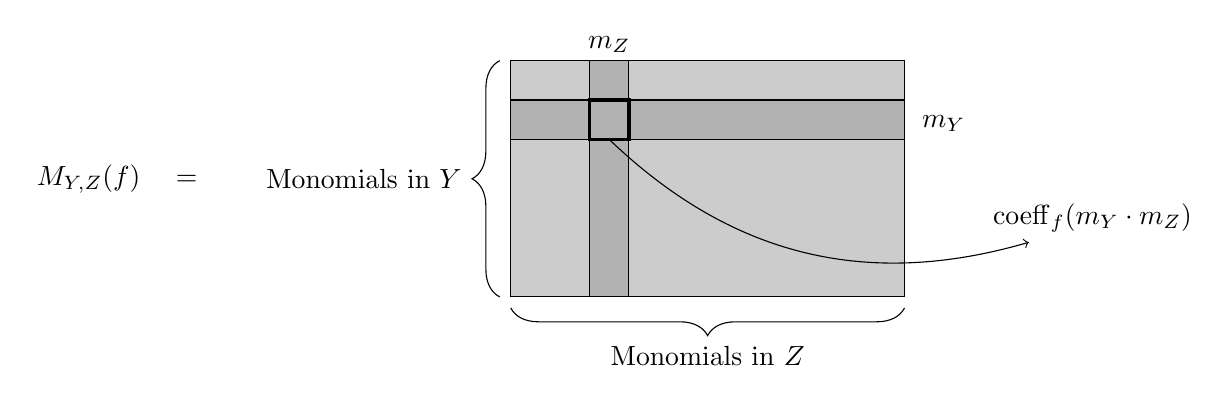
\begin{tikzpicture}
\node at (-5,1.5) {$M_{Y,Z}(f) \quad= $};
\draw[fill=black!20] (0,0) rectangle (5,3);

\draw[decorate,decoration={brace,amplitude=10pt,raise=4pt},yshift=0pt]
(0,0) -- (0,3);
\node[anchor=east] at (-0.5,1.5) {Monomials in $Y$};
\draw[decorate,decoration={brace,amplitude=10pt,mirror, raise=4pt},yshift=0pt] 
(0,0) -- (5,0);
\node[anchor=north] at (2.5,-0.5) {Monomials in $Z$};

\draw[fill=black!30] (1,0) rectangle (1.5,3);
\node at (1.25,3.2) {$m_Z$};

\draw[fill=black!30] (0,2) rectangle (5,2.5);
\node at (5.5,2.2) {$m_Y$};

\draw[very thick] (1,2) rectangle (1.5,2.5);

\node[anchor=west] at (6,1) {$\mathrm{coeff}_f(m_Y \cdot m_Z)$}
edge[<-,bend left] (1.25,2);
\end{tikzpicture}

\noindent
We shall use $\CM{Raz}_{Y,Z}(f)$ to denote the rank of $M_{Y,Z}(f)$. \\


Here are some basic properties of the partial derivative matrix which would be extremely useful in later calculations.

\begin{observation}[Sub-additivity]\label{obs:pdm-subadditivity}
	For any partition $X = Y \sqcup Z$ and any pair of multilinear 
	polynomials $f$ and $g$ in $\FF[X]$ we have 
$\CM{Raz}_{Y,Z}(f+g) \spaced{\leq} \CM{Raz}_{Y,Z}(f) \spaced{+} \CM{Raz}_{Y,Z}(g)$.
\end{observation}
\begin{proof}
Follows from the linearity of the matrix. 
\end{proof}

\begin{observation}[Multiplicativity]\label{obs:pdm-multiplicativity}
If $f_1 \in \F[Y_1,Z_1]$ and $f_2 \in \F[Y_2, Z_2]$ with $Y = Y_1 \sqcup Y_2$ and $Z = Z_1 \sqcup Z_2$, then
$$
\CM{Raz}_{Y,Z}(f_1\cdot f_2) \spaced{=} \CM{Raz}_{Y_1, Z_1}(f_1) \spaced{\cdot} \CM{Raz}_{Y_2, Z_2}(f_2).
$$
\end{observation}
\begin{proof}
  It is not hard to see that $M_{Y,Z}(f_1\cdot f_2)$ is the tensor product $M_{Y_1, Z_1}(f_1) \otimes M_{Y_2, Z_2}(f_2)$, and the rank of a tensor product of two matrices is the product of the ranks.
\end{proof}

\begin{observation}[Multiplication by univariates]\label{obs:pdm-mult-by-univariate}
For any $f \in \F[Y,Z]$ and any $g \in \F[Y]$, if $\F$ is large enough then we have that $\CM{Raz}_{Y,Z}(g \cdot f) \leq \CM{Raz}_{Y,Z}(f)$. 

By symmetry, the same is true when $g \in \F[Z]$. 
\end{observation}
\begin{proof}
  The evaluation dimension of $g \cdot f$ is at most the evaluation dimension of $g$ as any partial evaluation (by evaluating $Y$) of $g \cdot f$ is a scalar times a partial evaluation of $g$.
The observation follows from \autoref{lem:evalDim-to-coeffDim}.
\end{proof}


\begin{observation}[A trivial bound]\label{obs:pdm-upperbound}
For any multilinear polynomial $f$, we have  $\CM{Raz}_{Y,Z}(f) \spaced{\leq} 2^{\min(\abs{Y}, \abs{Z})}$.
\end{observation}
\begin{proof}
  The number of rows is $2^{\abs{Y}}$ and number of columns is $2^{\abs{Z}}$, and hence the rank is upper-bounded by the minimum.
\end{proof}

Let us get back to lower bounds for multilinear models, and attempt to use $\CM{Raz}_{Y,Z}(f)$ defined above. 
Unfortunately, there are examples of simple polynomials like $f = (y_1 + z_1)\dots (y_n + z_n)$ with $\CM{Raz}_{Y,Z}(f) = 2^n$. 
Raz's idea here was to look at $\CM{Raz}_{Y,Z}(f)$ for a \emph{random partition}, and show that with high probability the rank of the partial derivative matrix is far from full. 
As a toy example, we shall see why this has the potential to give lower bounds for depth-$3$ multilinear circuits. 

\begin{lemma}\label{lem:raz-depth-three}
Let $f(X) = \ell_1 \dots \ell_d$ be an $n$-variate multilinear polynomial. 
If $X = Y\sqcup Z$ is a random partition with $|Y| = |Z| = |X|/2$, then with high probability we have
$$
\CM{Raz}_{Y,Z}(f) \quad \leq \quad 2^{|X|/2} \cdot 2^{-|X|/16}.
$$
\end{lemma}

It is to be noted that we should expect a random polynomial to be full-rank with respect to any partition, so the measure $\CM{Raz}_{Y,Z}(f)$ is expected to be $2^{|X|/2}$ which should yield a lower bound of $2^{\Omega(|X|)}$. 

\begin{proof-sketch}
Without loss of generality we can assume that each $\ell_i$ depends on at least two variables as removing the $\ell_i$'s that depend on just one variable does not alter $\CM{Raz}_{Y,Z}(f)$ with respect to any partition. 
Let $|X| = n$. 

Using \autoref{obs:pdm-multiplicativity}, $\CM{Raz}_{Y,Z}(f) \leq 2^d$ and hence if $d < n/3$ then we are done. 
Hence assume that $d \geq n/3$. 
By a simple averaging argument, there must hence be at least $d/4$ of the $\ell_i$'s that depend on at most $3$ variables; we shall refer to these as the \emph{small} $\ell_i$'s. 

Since the partition is chosen at random, on expectation a quarter of the small $\ell_i$'s would have all its variables mapped to either $Y$ or $Z$, hence not contributing to $\CM{Raz}_{Y,Z}(f)$. 
Therefore, with high probability,
$$
\CM{Raz}_{Y,Z}(f) \quad \leq \quad 2^{d} \cdot 2^{-d/16} \spaced{\leq} 2^{n/2} \cdot 2^{-n/16}.
$$
\end{proof-sketch}

More generally, if $f = g_1(X_1)\dots g_t(X_t)$ where the $X_i$'s are mutually disjoint, then a random partition is very unlikely to partition all the $X_i$'s into almost equal parts. 
This naturally calls for using the multilinear log-product representation from \autoref{lem:mult-logproduct} for the case of multilinear formulas. The rest of this section would be proof of Raz's wonderful result \cite{raz2004}. 

\begin{theorem}[\cite{raz2004}] \label{thm:raz-ml-det}
Any multilinear formula computing $\Det_n$ or $\Perm_n$ must be of size $n^{\Omega(\log n)}$. 
\end{theorem}

The proof would be as outlined. If $f$ is computable by a size $s$ multilinear formula, then by \autoref{lem:mult-logproduct} we know that $f$ admits a log-product representation:
\[
f \spaced{=} \sum_{i=1}^{s+1} f_{i1} \cdots f_{i\ell}
\]
Using this, we shall first obtain an upper-bound on $\CM{Raz}_{Y,Z}(f)$ for a random partition $X = Y \sqcup Z$ by showing that any single log-product is far from full-rank. Finally, for $\Det_n$ or $\Perm_n$, we shall prove a lower bound on $\CM{Raz}_{Y,Z}$ for most partitions and that would complete the proof. 

In the original paper of \cite{raz2004}, Raz considered \emph{balanced} partitions $X = Y \sqcup Z$ with $|Y| = |Z| = |X|/2$ but this complicates issues because each variables are not independently assigned to $Y$ or $Z$. However, there is a slightly simpler analysis when we just independently assign each variable to $Y$ or $Z$ and deal with the possible imbalance later on. This trick was communicated to us by Srikanth Srinivasan. 


\subsection{Log-products are far from full-rank on a random
  partition}

The main technical part of the proof is to show that log-product multivariate polynomials are far from full-rank under a random partition of variables. 
This would let us show that a sum of log-product multivariate polynomials cannot be full rank unless it is a very large sum.\\

{\bf Main idea: } Suppose $f = g_1 \dots g_t$ where each $g_i \in \F[X_i]$. 
Let $X = Y \sqcup Z$ be a random partition, obtained by assigning each variable $x\in X$ independently to $Y$ or $Z$ with probability $1/2$ each. 
Let $Y_i = Y \intersection X_i$ and $Z_i = Z \intersection X_i$ and say $d_i = \abs{\frac{|Y_i| - |Z_i|}{2}}$ measure the imbalance between the sizes of $Y_i$ and $Z_i$. We shall say $X_i$ is $k$-imbalanced if $d_i \geq k$. 
Let $b_i = \frac{|Y_i| + |Z_i|}{2} = \frac{|X_i|}{2}$.

Suppose the partition was such that $|Y| = |Z|$ (as considered originally by Raz), then by \autoref{obs:pdm-multiplicativity} we know that 
\begin{eqnarray*}
\CM{Raz}_{Y,Z}(f) & = & \CM{Raz}_{Y_i,Z_i}(g_1) \dots \CM{Raz}_{Y_i,Z_i}(g_t)\\
 & \leq & 2^{\min(|Y_1|,|Z_1|)} \cdots  \cdot 2^{\min(|Y_t|,|Z_t|)}\\ 
 & = & 2^{b_1  - d_1} \cdots 2^{b_t - d_t} = \frac{2^{|X|/2}}{2^{d_1 + \dots + d_t}}.
\end{eqnarray*}

Hence, even if one of the $X_i$'s is a little imbalanced, then the product is far from full-rank. 

\autoref{lem:mult-logproduct} shows that the size of $X_i$ decreases slowly with $i$, and it is not hard to show that $\abs{X_i} \geq \sqrt{\abs{X}}$ for $i \leq t'\eqdef\frac{\log{\abs{X}}}{100}$. 
We wish to show that the probability that none of $g_i$ (for $i\leq t'$) is $k$-unbalanced for $k = \abs{X}^{1/20}$ is very small (inverse polynomially small). Since we have $t = \Theta(\log n)$ such independent events, the probabilty that \emph{none} of the $g_i$'s are $k$-unbalanced will be much smaller. \\

In the original setting of balanced partitions, these events are not exactly independent but one can make the calculations work out (using basic properties of hypergeometric distributions). But we'll work with partitions obtained by assigning each variable independently to $Y$ or $Z$. 

Let $\mathcal{E}_i$ be the event that $g_i$ is \emph{not} $k$-unbalanced.
Since the variables of the $g_i$'s are variable disjoint, and each variable is independently assigned to $Y$ or $Z$, these events $\mathcal{E}_i$'s are independent. What is the probability that $\mathcal{E}_i$ holds? 
The event $\mathcal{E}_i$ is just the probability that  $|Y_i| \in \insquare{\frac{|X_i|}{2} -k , \frac{|X_i|}{2} +k}$. Even the probability of $|Y_i| = |X_i|/2$ is at most $O(1/\sqrt{X_i})$. Hence,
\[
  \Pr\insquare{\mathcal{E}_i} \spaced{\leq} \frac{2k}{\sqrt{X_i}} \spaced{\leq} O\inparen{\frac{2k}{\sqrt[4]{|X|}}}.
\]
Since $t = \Theta(\log n)$, and these are independent events, 
\begin{eqnarray*}
  \Pr\insquare{\mathcal{E}_1\wedge \dots \wedge \mathcal{E}_{t'}} & \leq & \abs{X}^{-\epsilon \log \abs{X}} \quad\text{for some $\epsilon > 0$}.
\end{eqnarray*}

Now suppose we further condition this on the event that $|Y| = |Z|$, how different can the above probability become?
\begin{align*}
  \Pr\insquare{\mathcal{E}_1\wedge \dots \wedge \mathcal{E}_{t'}} & \geq  \Pr\insquare{\mathcal{E}_1\wedge \dots \wedge \mathcal{E}_{t'} \mid |Y| = |Z|} \cdot \Pr[|Y| = |Z|]\\
  \implies \Pr\insquare{\mathcal{E}_1\wedge \dots \wedge \mathcal{E}_{t'} \mid |Y| = |Z|} & \leq |X|^{-\epsilon \log |X|} \cdot \sqrt{|X|}
\end{align*}
and the $\sqrt{|X|}$ is inconsequential when we have an inverse-quasipolynomial error probability.
Therefore,
\[
 \Pr_{\substack{X = Y\sqcup Z\\|Y| = |Z|}}\insquare{\CM{Raz}_{Y,Z}(g_1\dots g_t) > 2^{(|X|/2) - |X|^{1/20}}}  \leq  \abs{X}^{-\epsilon \log \abs{X}}.
\]

Hence, if $g_1\dots g_t$ is a log-product multilinear polynomial, 
then with probability at least $\inparen{1 - |X|^{-\epsilon \log |X|}}$ 
we have that $\CM{Raz}_{Y,Z}(g_1\dots g_t) \leq 2^{(|X|/2) - |X|^{1/20}}$. 
Further, if $f$ is computable by a multilinear formula of size $s$ then, 
by \autoref{lem:mult-logproduct}, $f$ can be written as a sum of 
$(s+1)$ log-product multilinear polynomials. 
Hence, with probability 
at least $\inparen{1 - (s+1)|X|^{-\epsilon \log |X|}}$ we have that
$$\CM{Raz}_{Y,Z}(f) \spaced{\leq} (s+1) \cdot 2^{(|X|/2) - |X|^{1/20}}. $$
Hence, if $(s+1) < |X|^{(\epsilon/2) \log |X|}$, then with high 
probability a random partition would ensure 
$\CM{Raz}_{Y,Z}(f) \ll 2^{|X|/2}$. 
Let us record this as a lemma.


\begin{lemma}\label{lem:multformula-lowrank}
  Let $f \in \F[X]$ be computed by a multilinear formula of size $s < |X|^{(\epsilon/2) \log |X|}$ for a small enough constant $\epsilon > 0$. 
Then with probability at least $(1 - |X|^{-(\epsilon/2)\log |X|})$ we have $$\CM{Raz}_{Y,Z}(f) \spaced{\leq} (s+1)\cdot 2^{|X|/2} \cdot 2^{-|X|^{1/20}}$$ for a random partition $X = Y \sqcup Z$ with $|Y| = |Z| = |X|/2$.
\end{lemma}

\subsection{$\Det_n$ and $\Perm_n$ have large rank}

The last step of the proof would be to find an explicit polynomial whose partial derivative matrix under a random partition has large rank. 
As earlier, our candidate polynomial would be $\Det_n$ or $\Perm_n$. 
Unfortunately, both these polynomials are over $n^2$ variables and degree $n$. 
It is not hard to verify that the rank of the partial derivative matrix of $\Det_n$ or $\Perm_n$ can never be greater than $2^{2n}$. 
Hence directly using \autoref{lem:multformula-lowrank}, we would have $2^{O(n)}$ competing with $2^{n^2/2 - n^{O(1)}}$ which is simply futile. 
A simple fix is to first randomly restrict ourselves to fewer variables and then apply \autoref{lem:multformula-lowrank}. 

Let $\tilde{X} = \set{x_{11},\ldots, x_{nn}}$, and let us assume $n = 2m$ is even. We shall interpret all other variables as ``scalars'' by making our field $\mathbb{K} = \F\inparen{\setdef{x_{ij}}{i\neq j}}$ instead. If we had a multilinear formula of size $s$, over $\F$, computing $\Det_n$ then we also have a multilinear formula, over $\mathbb{K}$, of size at most $s$. We shall apply \autoref{lem:det-raz-lowerbound} for this circuit.

However, we show that for every balanced partition $\tilde{X} = Y \sqcup Z$ the partial derivative matrix (over $\mathbb{K}$) has full-rank. We will prove that the matrix has full-rank by showing that it has full-rank even after a substitution of the variables $\setdef{x_{ij}}{i\neq j}$. Consider the following restriction:
\begin{eqnarray*}
f & = & \Det \insquare{ \begin{array}{ccccc}
y_1 & 1   &        &     &    \\
1   & z_1 &        &     &    \\
    &     & \ddots &     &    \\
    &     &        & y_m &1   \\
    &     &        & 1   &z_m 
  \end{array}}\\
 &= & (y_1z_1 - 1)\dots (y_mz_m - 1).
\end{eqnarray*}
It is easy to check that $\CM{Raz}_{Y,Z}(f) = 2^m$. 

\begin{lemma}\label{lem:det-raz-lowerbound}
  For every balanced partition $\tilde{X} = Y \sqcup Z$ with $|Y| = |Z| = m = n/2$, we have $\CM{Raz}_{Y,Z}(\sigma(\Det_n)) = 2^m$. 
\end{lemma}


Combining \autoref{lem:det-raz-lowerbound} with \autoref{lem:multformula-lowrank}, we have the following theorem. 

\begin{theorem}[\cite{raz2004}] Any multilinear formula computing $\Det_n$ or $\Perm_n$ must be of size $n^{\Omega(\log n)}$. \qed
\end{theorem}

\subsection{Constructing a full-rank polynomial}\label{sec:fullrankpoly}

As alluded to earlier,  if $f$ is a random polynomial, then for any partition $X = Y \sqcup Z$ with $|Y| = |Z| = |X|/2$ we expect $\CM{Raz}_{Y,Z}(f) = 2^{|X|/2}$. 
Can we construct such a polynomial explicitly? 
This was first answered by Raz~\cite{Raz06}, and the construction was later simplified by Raz and Yehudayoff~\cite{ry08} and we shall describe the latter here. \\

{\bf Main idea:} Suppose you know the partition as $Y = \inbrace{y_1,\dots, y_n}$ and $Z = \inbrace{z_1,\dots, z_n}$, then building a polynomial such that $M_{Y,Z}(f)$ is full-rank is easy --- just take $f = (y_1z_1 + 1)\dots (y_n z_n + 1)$ which makes $M_{Y,Z}(f)$ the identity matrix. 
What we would like is to have one such copy for every partition, and we would also like to build it in a way so that $f$ can be computed in $\VP$. \\

The first attempt is to build the polynomial inductively for every partition into two equal parts, but ``remembering'' partial partitions take too much memory (similar to the situation we had in \autoref{thm:det-abp}). 
Raz and Yehudayoff instead use a different construct that, rather than being based on partitions, is instead based on Dyck-strings or well-matched parentheses. 

The language $\mathrm{Dyck}(n)$ refers to strings of length $2n$ over symbols `$($' and `$)$' that is well-matched in the natural way. 
That is ``()()'' and ``(())'' belong to $\mathrm{Dyck}(2)$ but not ``())(''. 
Raz and Yehudayoff come up with a natural map to convert every such string to a full-rank polynomial, and we shall just state this by example. 
\begin{eqnarray*}
\Omega(\text{``(())''}) & = & (x_1x_4 + 1)\cdot (x_2x_3 + 1)\\
\Omega(\text{``()()''}) & = & (x_1x_2 + 1)\cdot (x_3x_4 + 1)
\end{eqnarray*}
That is, if the opening bracket at position $i$ is closed at position $j$, then there is a factor $(x_ix_j + 1)$. 
Let us define the polynomial as follows:
\[
f(x_1,\dots, x_{2n}) \spaced{=} \sum_{s\in \mathrm{Dyck}(n)} \Omega(s) 
\]
Let us attempt to compute the polynomial using a small circuit in the following natural inductive manner. 
\[
f_{i,j}(\vecx) \spaced{=} \begin{cases}
(x_ix_j+1) & \text{if $j = i+1$}\\
0 & \text{if $j-i$ is even}\\
(x_ix_j+1) \cdot f_{i+1,j-1} &\\
 \spaced{+} \sum\limits_{r=i+1}^{j-1} f_{i,r}\cdot f_{r+1,j} & \text{otherwise}
\end{cases}
\]
However, $f_{1,2n}$ is \emph{not equal} to the polynomial $f$ as the term corresponding to ``()()()$\dots$()'' has coefficient $1$ in $f$ but is $C_n$, the $(n-1)$-th Catalan number. 
Nevertheless, this inductively defined polynomial $f_{1,2n}$ has most of the properties we need. 
Raz and Yehudayoff take a slight variant of it by adding a few auxiliary variables $\inbrace{\omega_{i,j,k},\omega_{i,j}}$ to build the following polynomial over the field $\F(\setdef{\omega_{i,j,k},\omega_{i,j}}{i,j,k\in [2n]})$. 
\[
\tilde{f}_{i,j}(\vecx) \spaced{=} \begin{cases}
(x_ix_j+1) & \text{if $j = i+1$}\\
0 & \text{if $j-i$ is even}\\
(x_ix_j+1) \cdot \tilde{f}_{i+1,j-1} \omega_{i,j}&\\
 \spaced{+} \sum\limits_{r=i+1}^{j-1} \tilde{f}_{i,r}\cdot \tilde{f}_{r+1,j} \cdot \omega_{i,r,j} & \text{otherwise}
\end{cases}
\]

\begin{lemma}[\cite{ry08}]\label{lem:fullrankpoly}
The polynomial $\tilde{f} = \tilde{f}_{1,2n}$ has the property that for every $X = Y \sqcup Z$ with $|Y| = |Z| = |X|/2$ we have $\CM{Raz}_{Y,Z}(\tilde{f}) = 2^{|X|/2}$. 
\end{lemma}
\begin{proof}
The proof shall be over induction on $n$. 
For the base case, statement is obviously true for $n = 1$ as $\tilde{f} = (x_1x_2 + 1)$ in this case. 

Suppose $n > 1$, and let $X = Y \sqcup Z$ be any partition with $|Y| = |Z| = |X|/2$. 
Then, either both $x_1$ and $x_{2n}$ belong to the same side of the partition, or they belong to different sides. 
Let us handle each case separately. 

\begin{description}
\item{Case 1:  $x_1$ and $x_{2n}$ are in different parts}. 

Then, polynomial $\tilde{f}$ where we set $\omega_{1,i,2n} = 0$ for all $i$. 
Under this substitution, $\tilde{f}$ is equal to $(x_1x_{2n}+ 1)\cdot \tilde{f}_{2,2n-1}$. 
By induction, we know that $\tilde{f}_{2,2n-1}$ is full-rank under equal sized partition and hence so is $(x_1 x_{2n} + 1) \cdot \tilde{f}_{2,2n-1}$. 
As setting variables to zero can only reduce the rank, it follows that $M_{Y,Z}(\tilde{f})$ must be full-rank as well. 

\item{Case 2:  $x_1$ and $x_{2n}$ are in the same part}. 

Since $|Y| = |Z| = |X|/2$, there must be some intermediate point $r$ such that the two intervals $[1,r]$ and $[r+1,2n]$ are both split evenly by $Y$ and $Z$. 
Using induction on each of these smaller intervals again, we get that $M_{Y,Z}(\tilde{f})$ is full-rank again. 
\end{description}
\end{proof}

This is one of the very few polynomials that we are aware of that can be computed by polynomial sized arithmetic circuits, but is not known to be computable by polynomial size ABPs. 

\section{Stronger lower bounds for constant depth multilinear formulas}

Looking back at \autoref{lem:multformula-lowrank}, we see that whenever $f(X)$ is computable by a size $s$ multilinear formula $\CM{Raz}_{Y,Z}(f)$ is exponentially smaller than $2^{|X|/2}$ with probability $\inparen{1 - s\cdot |X|^{-\epsilon \log |X|}}$. 
Hence we had to settle for a $n^{\Omega(\log n)}$ lower bound not because of the rank deficit but rather because of the bounds in the probability estimate. 
Unfortunately, this lower bound technique cannot yield a better lower bound for multilinear formulas as we have already seen (in \autoref{sec:fullrankpoly}) that there are explicit examples of polynomials computable by poly-sized multilinear circuits with $\CM{Raz}_{Y,Z}(f) = 2^{|X|/2}$ under \emph{every} partition. 
However, the probability bound can be improved in the case of constant depth multilinear circuits to give stronger lower bounds. 


Note that \autoref{lem:multformula-lowrank} was proved by considering \emph{multilinear log-products} (\autoref{defn:mult-logproduct}) as the building blocks. 
To show that a multilinear log product $g_1(X_1)\dots g_{\ell}(X_\ell)$ has small rank under a random partition, we argued that the probability that all the $X_i$'s are partitioned in a roughly balanced fashion is quite small. 
This was essentially done by thinking of this as $\ell = O(\log n)$ close-to-independent events, each with probability $1/\mathrm{poly}(n)$. 

If $\ell$ was much larger than $\log n$ (with other parameters being roughly the same), it should be intuitively natural to expect a much lower probability of all the $X_i$'s being partitioned in a roughly balanced manner. 
This indeed is the case for constant depth multilinear circuits, and we briefly sketch the key points where they differ from the earlier proof. 
The first is an analogue of \autoref{defn:mult-logproduct} in this setting. 

\begin{definition}\label{defn:mult-t-prod}
A multilinear polynomial $f$ is said to be a \emph{multilinear $t$-product} if $f$ can be written as $f = g_1\dots g_t$ with the following properties:
\begin{itemize}
\item The variable sets of the $g_i$ are mutually disjoint
\item Each $g_i$ non-trivially depends on at least $t$ variables
\end{itemize}
\end{definition}

\begin{lemma}\label{lem:mult-t-prod-rep}
Let $f$ be a multilinear polynomial of degree $d$ over $n$ variables that is computed by a depth-$\Delta$ multilinear formula $\Phi$ of size $s$. 
Then, $f$ can be written as a sum of at most $s$ multilinear $t$-products for $t = \inparen{n/100}^{1/2\Delta}$, and a multilinear polynomial of degree at most $n/100$.  
\end{lemma}
\begin{proof}
If $d < n/100$, then the lemma is vacuously true. 
Since $\Phi$ is a formula of depth $\Delta$ and computes a polynomial of degree $d > n/100$, there must be at least one product gate $v$ of fan-in at least $\inparen{\frac{n}{100}}^{1/\Delta} = t^2$. 
Then similar to \autoref{lem:mult-logproduct}, 
$$
f \quad=\quad \Phi_v \cdot f'  + \Phi_{v=0}
$$
As $\Phi_v$ is a product of $t^2$ polynomials, by grouping the factors together we have that $\Phi_v \cdot f'$ is a multilinear $t$-product. 
Further, $\Phi_{v=0}$ is a multilinear polynomial that is computable by a depth-$\Delta$ formula of smaller size and we can induct on $\Phi_{v=0}$. 
\end{proof}

\begin{lemma}\label{lem:mult-const-depth-upper-bound}
Let $f(X)$ be an $n$-variate polynomial computed by a depth-$\Delta$ multilinear formula of size $s$. 
If $X = Y \sqcup Z$ is a randomly chosen partition with $|Y| = |Z| = n/2$, then with probability at least $(1 - s \cdot \exp({-n^{\Omega(1/\Delta)}}))$ we have
$$
\CM{Raz}_{Y,Z}(f) \quad\leq\quad (s+1) \cdot 2^{n/2} \cdot \exp(-n^{\Omega(1/\Delta)}).
$$
\end{lemma}
\begin{proof-sketch}
By \autoref{lem:mult-t-prod-rep}, we have that $f$ can be written as $g_0 + g_1 + \dots + g_s$ where $\deg(g_0) \leq n/100$ and $g_1,\dots, g_s$ are multilinear $t$-products. 
Note that since $g_0$ is a multilinear polynomial of degree at most $(n/100)$, the number of monomials in $g_0$ is at most $\binom{n}{n/100} \leq 2^{n/10}$. 
Hence, $\CM{Raz}_{Y,Z}(g_0) \leq 2^{n/10}$. 

For the other $g_i$'s, we can bound the probability that $\CM{Raz}_{Y,Z}(g_i)$ is large in a very similar fashion as in \autoref{lem:multformula-lowrank}, as the probability that all the factors of $g_i$ are partitioned in a balanced manner is the intersection of $t$ independent events. 
By very similar estimates, this probability can be bounded by $(1/\mathrm{poly}(n))^t$. 
Hence, with high probability 
$$
\CM{Raz}_{Y,Z}(f) \spaced{\leq} \CM{Raz}_{Y,Z}(g_0) + \dots + \CM{Raz}_{Y,Z}(g_s) \spaced{\leq} (s+1)\cdot 2^{n/2} \cdot \exp(-n^{\Omega(1/\Delta)}).
$$
\end{proof-sketch}

Combining \autoref{lem:mult-const-depth-upper-bound} with \autoref{lem:det-raz-lowerbound}, we have the following theorem of Raz and Yehudayoff. 

\begin{theorem}[\cite{raz-yehudayoff}]
Any multilinear formula of depth $\Delta$ computing $\Det_n$ or $\Perm_n$ must be of size $\exp(n^{\Omega(1/\Delta)})$.  \qed
\end{theorem}



%%% Local Variables: 
%%% mode: latex
%%% TeX-master: "fancymain"
%%% End: 


\include{chap_multi-k-ic}

\include{chap_multiFormABPSep}

%% multilinear depth hierarchy theorem of Chillara-Engels-Limaye-Srinivasan

\chapter{Tensor rank and formula lower bounds}\label{chap:tensorrk}

In this chapter, we will establish an apriori surprising connection between lower bounds for homogeneous arithmetic formula and constructing explicit tensors of full rank.
The chapter is based on a result of Raz~\cite{raz10}.

\section{Tensors}

Tensors are natural \emph{higher dimensional} analogues of matrices.
A matrices is nothing but a two dimensional array filled in with numbers from some underlying field.
A tensor is a higher dimensional version of this, where we have an $d$-dimensional cuboid filled with numbers.
A tensor $T$ is a map of the form
\[
T: [m_1] \times \cdots \times [m_d] \longrightarrow \F
\]
the same way an $m\times n$ matrix a map from $[m] \times [n] \rightarrow \F$.
However, if one wants to understand a tensor more functionally (similarly to how it is useful to think of matrices as linear transformations on vector spaces), it is more natural to extend this definition linearly as follows.

\begin{definition}[Tensor]\label{defn:tensor}
A tensor $T$ is a map of the form 
\[
T: V_1 \times \cdots \times V_d \longrightarrow \F
\]
where each $V_i$ is a vector space over $\F$, of say dimension $m_i$, which is linear in every coordinate i.e.
\[
T(\vecv_1, \ldots,\alpha\vecv_i + \beta\vecv_i', \ldots, \vecv_d) = \alpha T(\vecv_1, \ldots,\vecv_i, \ldots, \vecv_d) + \beta T(\vecv_1, \ldots,\vecv_i', \ldots, \vecv_d).
\]
The parameter $d$ is called the \emph{order} of the tensor, and we say that the \emph{shape of $T$} is $m_1 \times \cdots \times m_d$. 
\end{definition}
Since a tensor is linear in every coordinate, it suffices to specify the image of $T$ at the basis of $V_1 \times \cdots \times V_d$ and extend it linearly.
So a tensor can indeed be thought of as filling up a $d$-dimensional array of shape $[m_1]\times \cdots \times [m_d]$ by field elements, the same way an $m\times n$ matrix is specified by an $m\times n$ array filled up with field elements.
Indeed, a matrix is nothing but an order-$2$ tensor.

It would sometimes be useful to switch between the two notions of thinking of a tensor as a multilinear map from $V_1 \times \cdots \times V_d$ to $\F$ and thinking a tensor as just a map from $[m_1] \times \cdots \times [m_d]$.
So throughout this chapter, we shall fix a basis $\set{\vece_{i1},\ldots, \vece_{im_i}}$ for $V_i$ and when we shall use $T[j_1,\ldots, j_d]$ to really denote $T(\vece_{1j_1},\ldots, \vece_{dj_d})$.

\subsection{Tensors as polynomials}

In our setting, it would be useful to think of tensors as a restricted form of multilinear polynomials that are called \emph{set-multilinear polynomials}.

\begin{definition}[Set-multilinear polynomials]\label{defn:set-multilinear}
  Let $\vecx = \vecx_1 \sqcup \cdots \sqcup \vecx_d$ be a partition of variables and let $|\vecx_i| = m_i$.
A polynomial $f(\vecx)$ is said to be \emph{set-multilinear} with respect to the above partition if every monomial $m$ in $f$ satisfies $\abs{m \intersection X_i} = 1$ for all $i \in [d]$.
\end{definition}
In other words, each monomial in $f$ picks up at most one variable from each part in the partition. It is easy to see that many natural polynomials such as $\Det$ or $\Perm$ or $\NW$ are all set-multilinear for an appropriate partition of variables. 

\begin{observation}\label{obs:tensor-to-sml}
  For any tensor $T$ of shape $[m_1] \times \cdots \times [m_d]$, we can associate a set-multilinear polynomial $f(\vecx)$ with $\vecx = \vecx_1 \sqcup \cdots \sqcup \vecx_d$ and $\vecx_i = \set{x_{i1}, \ldots, x_{im_i}}$ as
\begin{equation}\label{eqn:tensor-sml}
f(\vecx) \spaced{=} \sum_{\substack{1 \leq i_j \leq m_j\\ \forall j \in [d]}}  T(i_1,\ldots, i_d) \cdot x_{1i_1}\cdots x_{di_d}.
\end{equation}
\end{observation}

Another representation is to just use a single variable $x_j$ for a part $\vecx_j$ and use higher powers.
That way, we can associate the following polynomial with a tensor $T$:
\begin{equation}\label{eqn:tensor-to-prod-univariates}
f(x_1,\ldots, x_d) \spaced{=} \sum_{\substack{1 \leq i_j \leq m_j\\ \forall j \in [d]}}  T(i_1,\ldots, i_d) \cdot x_{1}^{i_1}\cdots x_{d}^{i_d}.
\end{equation}
The same also holds in the other direction where we can interpret any set-multilinear polynomial as an appropriate tensor. 


\subsection{Rank of a tensor}

Just like any matrix has a natural definition of \emph{rank}, there is an analogue for tensors as well.
The rank of a matrix $M$ can be defined as the smallest $r$ for which $M$ can be written as a sum of $r$ matrices of rank $1$.
A rank-$1$ matrix is just a matrix of the form $\vecu \vecv^T$ where the $(i,j)$-th entry is $u_iv_j$.
We shall abuse\footnote{it is abuse because it is really a tensor product of $\vecu$ and $\vecv^T$.}
notation and use $\vecu \otimes \vecv$ to denote the order-$2$ tensor $T$ where $T[i,j] = u_i v_j$.
This naturally generalizes to higher order as well.

\begin{definition}[Elementary tensors, and tensor rank]
  For $\vecv_1\in V_1, \ldots, \vecv_d \in V_d$, define the tensor $\vecv_1 \otimes \cdots \otimes \vecv_d$ to be the tensor $E$ given by
\[
E[j_1,\ldots, j_d] = (\vecv_1)_{j_1} \cdots (\vecv_d)_{j_d}.
\]
We shall call such tensors as \emph{elementary tensors} or \emph{rank-$1$ tensors}. 

For an arbitrary tensor $T$, the \emph{tensor rank of $T$}, denoted by $\rank(T)$, is the smallest $r$ such that $T$ can be expressed as a sum of $r$ elementary tensors. 
\end{definition}

\noindent 
What do elementary tensors look like as polynomials?
Let us consider the \emph{set-multilinear} polynomial setting as in \eqref{eqn:tensor-sml}.
It is easy to see that a rank-$1$ tensor is precisely a \emph{set-multilinear} product of linear forms such as
\[
f(\vecx) \spaced{=} \ell_1(\vecx_1) \cdots \ell_d(\vecx_d)
\]
where each $\ell_i(\vecx_i)$ is a linear form in the variables in $\vecx_i$. \\

In the setting of \eqref{eqn:tensor-to-prod-univariates}, it is easy to see that a rank-$1$ tensor is precisely a \emph{product of univariates} such as
\[
f(\vecx) \spaced{=} f_1(x_1)\cdots f_d(x_d).
\]
\noindent
Hence the following three questions are equivalent:
\begin{itemize}
\setlength\itemsep{0em}
\item Given a tensor $T$, find its rank. 
\item Given a set-multilinear polynomial $f$, find the smallest set-multilinear $\SPS$ circuit computing it. 
\item Given a polynomial $f$, find the smallest expression as a sum of product of univariates.
\end{itemize}

However, unlike matrices, computing the rank of even an order-$3$ tensor is $\NP$-hard \cite{h90}.
But one could still ask if we can prove good upper or lower bounds for some specific tensors, or try to find a tensor with large rank.
But before that, let us look at some basic properties that tensor rank satisfies.

\subsection*{Properties of  tensor rank}

The following are a couple of basic properties that follows almost immediately from the definitions.

\begin{lemma}[Sub-additivity of tensor rank]\label{lem:tensor-subadditivity}
  Let $T_1$ and $T_2$ be two tensors of the same shape and order.
Then, if $T = T_1 + T_2$, then $\rank(T) \leq \rank(T_1) + \rank(T_2)$.
\end{lemma}

\begin{lemma}[Sub-multiplicativity of tensor rank]\label{lem:tensor-submultiplicativity}
  Let $T_1: V_1 \times \cdots \times V_{d_1} \rightarrow \F$ and $T_2: W_1 \times \cdots \times W_{d_2} \rightarrow \F$ be two tensors.
Then if $T = T_1 \otimes T_2$ given by
\[
T[i_1,\ldots, i_{d_1},j_1,\ldots, j_{d_2}] = T_1[i_1,\ldots, i_{d_1}] \cdot T_2[j_1,\ldots, j_{d_2}],
\]
then $\rank(T) \leq \rank(T_1) \cdot \rank(T_2)$. 
\end{lemma}

% \begin{exercise}
%   Show that in fact $\rank(T_1 \otimes T_2) = \rank(T_1) \cdot \rank(T_2)$.
% \end{exercise}
% Actually, I thought this was easy but now I am not even convinced if this is true! Thanks to Jeroen Zuiddam for bringing this to my notice

\subsection{Upper bounds on tensor rank}

Let us consider an order-$d$ tensor $T$ of shape $n \times \cdots \times n$.
How large can $\rank(T)$ be?
One possible upper bound we could say is $n^d$.
Surely, the tensor is an $d$-dimensional array with just $n^d$ entries.
We can certainly write it as a sum of $n^d$ elementary tensors of the form $\vece_{j_1} \otimes \cdots \otimes \vece_{j_d}$.
So clearly $\rank(T) \leq n^d$.
But we can do a little better.
Consider the case when $d=2$, and we have an $n\times n$ matrix.
The bound on the rank is not $n^2$ but rather $n$.
This indicates that one should be able to do a bit better than $n^d$ for the general case.
Indeed we can.

\begin{lemma}\label{lem:tensor-rank-trivial-upperbound}
  Let $T$ be an order-$d$ tensor of shape $n\times \cdots \times n$.
Then, $\rank(T) \leq n^{d-1}$.
\end{lemma}
\begin{proof}
  Let us revisit the case when $d=2$, where we know an $n\times n$ matrix has rank at most $n$.
Interpreting this statement via \eqref{eqn:tensor-to-prod-univariates}, this implies that of $q(x_1,x_2)$ is a bi-variate with degree in each variable bounded by $n$, then $q$ can be written as
\[
q(x_1,x_2) = \sum_{i=1}^n g_i(x_1) h_i(x_2).
\]
Therefore, if $f(x_1,\ldots, x_d)$ is a polynomial with degree in each variable bounded by $n$, then we can write $f$ as
\begin{align*}
f(x_1,\ldots, x_d) &= \sum_{m \in \mathrm{Mon}\set{x_3,\ldots, x_d}} m \cdot q_m(x_1,x_2)\\
& = \sum_{m \in \mathrm{Mon}\set{x_3,\ldots, x_d}} m \cdot \inparen{\sum_{i=1}^n g_{m,i}(x_1) \cdot h_{m,i}(x_2)}
\end{align*}
which is a sum of product of univariates of top fan-in $n \cdot n^{d-2} = n^{d-1}$. 
\end{proof}

A counting argument would say that there do exist tensors of rank at least $n^{d-1}/d$ as each elementary tensor has $nd$ \emph{degrees of freedom} and an arbitrary tensor has $n^d$ \emph{degrees of freedom}.
One might think that the above upper bound of $n^{d-1}$ should be tight.
Bizarrely, it is not!
For example (cf.
\cite{p85}), the maximum rank of any tensor of shape $2\times 2 \times 2$ is $3$ and not $4$ as one might expect!
Tensor rank also behaves in some strange ways under \emph{limits} unlike the usual matrix rank.
But a big open question is to find explicit tensors of such large rank.

\begin{openproblem}
Can we find an explicit tensor $T: [n]^d \rightarrow \F$ of rank $n^{d(1 - o(1))}$?
\end{openproblem}

Raz's \cite{raz10} showed that in certain regimes, an answer to the above question would yield arithmetic formula lower bounds. 

\section{Tensor rank of small formulas}

From this section onwards, we shall assume the \emph{set-multilinear polynomial} interpretation of a tensor $T:[n]^d \rightarrow \F$ as described in~\eqref{eqn:tensor-sml}.
Hence our variables $\vecx$ is partitioned as $\vecx = \vecx_1 \sqcup \cdots \sqcup \vecx_d$ with $\abs{\vecx_i} = n$ for all $i\in [d]$.
The main motivating question would be the following:
\begin{quote}
If $f$ is a set-multilinear polynomial that is computed by a small formula, what can one say about its tensor rank?
\end{quote}

To begin with, let us restrict ourselves to certain structured formulas that in a sense \emph{respects} the partition defined. 

\begin{definition}[Set-multilinear formulas] A formula $\Phi$ is said
  to be a \emph{set-multilinear formula} if for every gate in the formula computes a set-multilinear polynomial.
\end{definition}

From the above definition, note that the set-multilinear formulas are a subclass of homogeneous formulas.
As in the multilinear setting, it is easy to see that set-multilinearity for formulas can be made a \emph{syntactic} restriction where each gate computes a tensor, with addition gates only adding ``alike'' tensors and multiplication gates multiplying disjoint tensors.

\begin{exercise}
  Show that set-multilinear formulas can, without loss of generality, be assumed to be syntactically set-multilinear formulas.
\end{exercise}

\noindent
An easier question to the one above would be the following:

\begin{quote}
  If $f$ is a set-multilinear polynomial that is computed by a small \emph{set-multilinear} formula, what can one say about its tensor rank?
\end{quote}

In the rest of this chapter, we shall prove the following result of Raz \cite{raz10}. 

\begin{theorem}[\cite{raz10}] \label{thm:raz-tensorrank-sml} Let
  $\Phi$ be a set-multilinear formula of size $s \leq n^c$ computing a polynomial $f(\vecx_1,\ldots, \vecx_d)$.
Then,
\[
\rank(f) \spaced{\leq} \frac{n^d}{n^{d/\exp(c)}}. 
\] 
\end{theorem}

In the setting when $d$ is small, Raz \cite{raz10} also showed that formulas can be converted to set-multilinear formulas with a modest cost. 

\begin{theorem}[\cite{raz10}]\label{thm:form-to-smlform}
  Suppose $d = O\pfrac{\log n}{\log\log n}$.
If $\Phi$ is a formula of size $s = \poly(n)$ that computes a set-multilinear polynomial $f(\vecx_1,\ldots, \vecx_d)$, then there is a \emph{set-multilinear} formula of $\poly(s)$ size that computes $f$ as well.
\end{theorem}

As a corollary, finding explicit tensors of almost full rank would imply super-polynomial formula lower bounds in the low-degree regime.

\begin{corollary}[\cite{raz10}]
  If $f(\vecx_1,\ldots, \vecx_d)$ is an explicit tensor of rank $n^{d(1- o(1))}$ with $\omega(1) = d = O\pfrac{\log n}{\log\log n}$, then any formula computing $f$ must be of super-polynomial size.
\end{corollary}

The above two theorems are of very different flavours and should really be thought of as two independent surprising results.
\autoref{thm:raz-tensorrank-sml} is a tensor-rank upper bound and \autoref{thm:form-to-smlform} is a structural result.
We shall first address \autoref{thm:raz-tensorrank-sml} in the next section and address \autoref{thm:form-to-smlform} after that.

\subsection{The tensor-rank upper-bound}

We shall now prove \autoref{thm:raz-tensorrank-sml}. The proof described here is not the original proof in \cite{raz10} but is an alternate proof by Suryajith Chillara, Mrinal Kumar and Ramprasad Saptharishi. 

\begin{proof}[Proof of \autoref{thm:raz-tensorrank-sml}]



For this we would need the slightly better depth reduction for homogeneous formulas (\autoref{thm:av-formulas}) of Saptharishi and Vinay \cite{saptharishivinay14}. We recall the statement here.
\begin{theorem*}[\autoref{thm:av-formulas}]
Let $f$ be a homogeneous $n$-variate degree $d$ polynomial computed by a size $s$ homogeneous formula. 
Then for any $0< t \leq d$, $f$ can be equivalently computed by a homogeneous $\Sigma\Pi^{[a]}\Sigma\Pi^{[t]}$ formula of top fan-in $s^{10(d/t)}$ where 
\[
a \geq \frac{1}{10}\pfrac{d}{t} \log t.
\]
\end{theorem*}
It is a fairly straightforward observation to see that the above theorem preserves multilinearity and set-multilinearity as well. We shall start with the set-multilinear formula $\Phi$ of size $s = n^c$ that computes the polynomial $f(\vecx_1,\ldots, \vecx_d)$ and apply \autoref{thm:av-formulas} for a suitable choice of $t$ (that shall be set shortly). 
Therefore we now have a set-multilinear expression of the form
\[
f \spaced{=} T_1 + \cdots + T_{s'}
\]
where $s' \leq s^{10(d/t)} = n^{10c(d/t)}$ and each $T_i = Q_{i1} \cdots Q_{ia_i}$ is a set-multilinear product. Let us fix one such term $T = Q_{1} \cdots Q_a$ and we know that this is a set-multilinear product with $a \geq \pfrac{d\log t}{10 t}$. Let $d_i = \deg(Q_i)$. By the sub-multiplicativity of tensor rank (\autoref{lem:tensor-submultiplicativity}) and the trivial upper bound (\autoref{lem:tensor-rank-trivial-upperbound}) we have
\begin{align*}
\rank(T) & \leq n^{d_1 - 1} \cdots n^{d_a - 1}\\
 & =  n^{d - a}\\
\implies \rank(f) & \leq s' \cdot n^{d-a} & \text{(~\autoref{lem:tensor-subadditivity})}\\
 & =  \pfrac{n^d}{n^{a - 10c(d/t)}}
\end{align*}
Let us focus on the exponent of $n$ in the denominator. Using the lower bound on $a$ from \autoref{thm:av-formulas}, we get
\begin{align*}
a - 10c(d/t) & \geq \frac{d\log t}{10t} - 10c\pfrac{d}{t}\\
& = \pfrac{d}{t} \inparen{\frac{\log t}{10} - 10c}\\
& = \pfrac{d}{2^{O(c)}}& \text{if we set $\frac{\log t}{10} = 11c$}\\
\implies \rank(f) & \leq \frac{n^d}{n^{d/\exp(c)}}
\end{align*}
which is what we set out to prove. 
\end{proof}

\subsection{Making formulas set-multilinear}

In this section we shall prove \autoref{thm:form-to-smlform}.
The proof would proceed in two steps, both of which are quite interested in their own right.
\begin{itemize}
\setlength\itemsep{0em}
\item {\bf Homogenization :} In the first step, we shall convert a
  formula that compute a homogeneous polynomial of degree $d$ in $n$ variables to a n homogeneous formula computing the same polynomial.
It would turn out that if $d = O(\log n)$, then this transformation only incurs a $\poly(n)$ blow-up in the size.
\item {\bf Set multilinearization :} In the second step, we show that
  for any homogeneous arithmetic formula that computes a set multilinear polynomial of degree $d$ in $n$ variables can be converted to a set-multilinear formula computing the same polynomial.
In this setting, if $d \leq O(\log n/\log \log n)$, the blow-up in the size of the formula will only be $\poly(n)$.
\end{itemize}

\subsubsection*{Homogenization of low-degree formulas}

\begin{lemma}[\cite{raz10}]\label{lem:formula-homogenization} Let $\Phi$ be a formula of size $s$ computing an $n$-variate homogeneous polynomial $f$ of degree $d$. Then, there is a \emph{homogeneous formula} $\Phi'$ computing $f$ of size at most $\poly\inparen{s,\binom{d+\log s}{d}}$. 

In particular, if $d = O(\log n)$ and $n = \poly(n)$ then we have $\mathrm{size}(\Phi') = \poly(n)$ as well. 
\end{lemma}
\begin{proof}
Recall that due to the depth reduction result of Brent and Spira (\autoref{lem:formula-depth-reduction}), we can assume without loss of generality that the fan-in of every gate in $\Phi$ at most $2$ and the depth of $\Phi$ is $O(\log s)$.
The construction of the new formula $\Phi'$ would have no surprises -- homogenize the formula $\Phi$ to obtain a circuit $C$ using the standard homogenization (\autoref{lem:homogenization}), and unravel the circuit to make it a formula in the most natural way. It is the analysis of the size that would give the lemma. 

\medskip

For every gate $v$ in $\Phi$, we have $d+1$ gates $(v, 0), (v, 2), \ldots, (v, d)$ in $C$.
Semantically, the polynomial computed at such a gate $(v, i)$ is the degree-$i$ homogeneous component of the polynomial computed at $v$ in $\Phi$. As in \autoref{lem:homogenization}, we shall connect these edges as follows:
\begin{eqnarray*}
v = u+w\quad\implies\quad (v, i) &=& (u, i) \spaced{+} (w,i)\quad\text{for all $i$}\\
v = u\times w\quad\implies\quad (v, i) &=& \sum_{j=0}^i (u,j)\cdot (w, {i-j}) \quad\text{for all $i$}
\end{eqnarray*}
Hence, we now have a homogeneous circuit $C$ that computes $f$ and has size at most $s' = O(sd^2)$. Furthermore, the depth of this circuit is at most twice the depth of the formula $\Phi$ which was $O(\log s)$. Hence $C$ is a homogeneous circuit of depth $O(\log s)$ and size $O(sd^2)$ computing $f$. 

To convert $C$ into a formula, we will do the natural operation of \emph{recomputing} a node whenever we need to reuse the computation. This is equivalent to duplicating every gate $(v,i)$ of $C$ as many times are there are paths from this gate to the root fo $C$.
Thus, in order to upper bound the size of the resulting formula, we will require an upper bound on the number of distinct paths from every gate $(v,i)$ of $C$ to its root.

\medskip

Currently, $C$ is a circuit because if $v$ is a product gate of $\Phi$ with children $u$ and $w$, then the out degree of $(u, j)$ and $(w, j)$ in $C$ could be more than $1$ as it \emph{contributes} to $(v,j')$ for all $j \leq j' \leq d$.
Hence, the resulting structure is a circuit and not a formula.
However, at sum gates, the out degree of the children continue to be $1$.
But this gives us a good understanding of the many paths from $(v,i)$ to the root in $C$.
Let $v\rightarrow v_1 \rightarrow \cdots \rightarrow v_r$ be the path from $v$ to the root ($=v_r$) in $\Phi$. Then, the paths from $(v,i)$ to $(v_r,d)$ will be of the form
\[
(v,i) \rightarrow (v_1,i_1) \rightarrow \cdots \rightarrow (v_r,i_r)
\]
where $i \leq i_1 \leq \cdots \leq i_r = d$.
But the number of such choices for $(i_1,\ldots, i_r)$ the same as the number of non-negative integer solutions to $b_1 + \cdots + b_r = d-i$ which is at most $\binom{r + d}{d}$.
We know that the circuit has depth at most $O(\log s)$ and hence $r \leq O(\log s)$.
Therefore, the number of paths from any $(v,i)$ to the root is at most $\binom{d + O(\log s)}{d}$.
Hence, if $\Phi'$ is the formula obtained by unravelling $C$, we have
\[
\mathrm{size}(\Phi') = \poly\inparen{s,\binom{d+\log s}{d}}.
\]
\end{proof}

\subsubsection*{Set-multilinearization of low-degree formulas}

We shall now show that a homogeneous formula can be converted to a set-multilinear formula with a cost that is affordable if $d$ is small. 

\begin{lemma}[Formula Set-multilinearization]\label{lem:formula set-multilinearization}
  Let $f(\vecx)$ be an $n$-variate degree set-multilinear polynomial with respect to the partition $\vecx = \vecx_1\sqcup \cdots \sqcup \vecx_d$ that is computed by a homogeneous formula $\Phi$ of size $s$.
Then, there exists a set-multilinear formula $\Phi'$ of size at most $2^{O(d\log \log s)}$ which computes $f$.

In particular, if $d = O\pfrac{\log n}{\log \log n}$ and $s = \poly(n)$ then the $\mathrm{size}(\Phi') = \poly(n)$.  
\end{lemma}
\begin{proof}
To start with, without loss of generality, let us assume that the formula $\Phi$ is fan-in $2$, homogeneous and has depth $O(\log s)$.
In the first step, we set multilinearize $\Phi$ in the obvious way to obtain a circuit $C$.
To this end, for every gate $v$ in $\Phi$, and vector $\veca = (a_1,\ldots, a_d) \in \{0,1\}^d$, there is a gate $(v, \veca)$ in $C$.
Semantically, the the polynomial at $(v,\veca)$ consists of the monomials in the polynomial computed at $v$ (in $\Phi$) which contain exactly one variable from the set $\vecx_i$ for every $i$ such that $a_i = 1$.
The edges in $C$ are connected in a natural way, namely for a gate $v$ with children $u$ and $w$, we have the following edges:
\begin{eqnarray*}
\text{$v = u + w$}\quad\implies\quad (v, \veca) &=& (u, \veca) \spaced{+} (w, \veca)\quad\text{for all $\veca$}\\
\text{$v = u \times w$}\quad\implies\quad (v, \veca) &=& \sum_{\vecb + \vecc = \veca} (u, \vecb)\cdot (w, \vecc) \quad\text{for all $\veca$}.
\end{eqnarray*}
 
Clearly, the size of $C$ is at most $2^d\cdot s$.
Moreover, the gates in $C$ which have out degree more than one are of the form $(u,\veca)$ where $u$ is a child of some multiplication gates at $\Phi$. 
The root of $C$ would now be $(\text{root},\mathbf{1})$. 

Like in the proof of \autoref{lem:formula-homogenization}, we now convert the circuit $C$ to a formula by replicating nodes whenever we need to reuse computations.
Hence, we would require as many copies of a gate $(v, \veca)$ as there are paths from $(v,\veca)$ to the root of $C$.
In order to bound the blow up in size in the process, we will prove an upper bound on the number of such paths.
Once again, let $v \rightarrow v_1 \rightarrow \cdots \rightarrow v_r$ be the path from $v$ to the root $(=v_r)$.
Then any path from $(v,\veca)$ to $(v_r,\mathbf{1})$ is of the form
\[
(v,\veca) \rightarrow (v_1,\veca_1) \rightarrow \cdots \rightarrow (v_r,\mathbf{1})
\]
with $\veca \leq \veca_1 \leq \cdots \leq \mathbf{1}$ in the point-wise sense.
Therefore, the number of paths from $(v,\veca)$ to the root is at most the number of sequences of ``increasing'' vectors $\veca_1, \cdots, \veca_r \in \set{0,1}^d$. Note that the number of such sequences is at most $r^d$ (why?)
and hence the number of paths from $(v,\veca)$ to the root is at most $2^{d\log r} = 2^{O(d\log\log s)}$.
Hence the size of the resulting formula $\Phi'$ is at most $s \cdot 2^{O(d \log\log s)}$. 
\end{proof}

\autoref{lem:formula-homogenization} and \autoref{lem:formula set-multilinearization} complete the proof of \autoref{thm:form-to-smlform}. 


%%% Local Variables: 
%%% mode: latex
%%% TeX-master: "fancymain"
%%% End: 





\part{Separations in the monotone world}

\include{chap_monABPCktSep}

\include{chap_monVPVNP}

%% Hrubes-Yehudayoff's nc-Formulas >> nc-mon-circuits

\part[Lower bounds for depth four circuits]{Lower bounds for depth four circuits:\\Shifted partial derivatives}

\include{chap_d4botfanin}

\include{chap_d4hom}

\part{Further applications of shifted partial derivatives}

\include{chap_SPDKeyPoints}

\include{chap_PSPD_more}

\chapter{The power of non-homogeneous depth three circuits}
\label{chap:d3nonhom}
A $\Sigma\Pi\Sigma$ circuit computes a polynomial of the form
\[
f\quad=\quad \sum_{i=1}^s \ell_{i1}\dots \ell_{iD}.
\]
If the circuit is non-homogeneous, the degree of the circuit $D$ could potentially be much larger than $\deg(f)$. \\

The class of depth three arithmetic circuits can compute polynomials
in non-trivial ways.
To illustrate a couple of examples, there is a homogeneous $\SPS$
circuit for $\Perm_n$ of size $2^{O(n)}$ called Ryser's Formula
\cite{rys63}
\begin{equation}\label{eqn:ryser}
\Perm_n \spaced{=} \sum_{S \subseteq[n]} (-1)^{n - |S|} \prod_{i=1}^n \inparen{\sum_{j\in S} x_{ij}}
\end{equation}
On the other hand, no $\SPS$ circuit for the $\Det_n$ significantly
better than writing it as a sum of $n!$ monomials was known (until
\cite{gkks13b}). 
Further, the elementary symmetric polynomials $\ESym_k(x_1,\dots,
x_n)$ of degree $k$ defined as
\[
\ESym_k(\vecx) \spaced{=} \sum_{\substack{S\subset \vecx\\|S| = k}} \prod_{x_i\in S}x_i
\]
can be computed by a non-homogeneous depth $3$ circuit of size
$O(n^2)$ over any characteristic zero field.
In stark contrast, \cite{nw1997} showed that any homogeneous depth $3$
circuit computing $\ESym_k$ requires size
$n^{\Omega(k)}$. \cite{nw1997} also showed a $2^{\Omega(n)}$ lower
bound for homogeneous depth $3$ circuits computing $\Perm_n$ or
$\Det_n$. 

Also, the results of \cite{gr00,grigoriev98} showed a $2^{\Omega(n)}$
lower bound for $\SPS$ circuits \emph{over finite fields} that compute
$\Det_n$ or $\Perm_n$.
All these results seemed to suggest that there perhaps is an
$2^{\Omega(n)}$ lower bound for $\SPS$ circuits computing $\Det_n$
over characteristic zero fields as well.
If it was true over finite fields, and for homogeneous $\SPS$
circuits, how much power can characteristic zero fields and
non-homogeneity add? 
As it turns out, quite a lot!

\begin{theorem}[\cite{gkks13b}] \label{thm:chasm-at-3} Let $f$ be an
  $n$-variate degree $d$ polynomial computed by an arithmetic circuit
  of size $s$ over any characteristic zero field.
  Then there is a $\SPS$ circuit of size $s' \leq s^{O(\sqrt{d})}$
  that computes $f$. 
\end{theorem}
\begin{corollary}[\cite{gkks13b}]\label{cor:det-sps}
There is a $\SPS$ circuit over $\Q$, the field of rational numbers, of size $n^{O(\sqrt{n})}$. 
\end{corollary}


The proof is quite short and comprises of two steps using known reductions, and going through a bizarre intermediate model of \emph{depth $5$ powering circuits}.
We present a longer route towards this result that perhaps sheds more light on the reduction.

\section{Handling non-homogeneous depth-$3$ circuits}\label{sec:non-hom-d3}

Non-homogeneous models are generally difficult to deal with in the
context of lower bounds.
A natural question to ask if any such non-homogeneous circuit can be
converted to a suitable homogeneous model which may then be attacked.
This was first studied by Shpilka and Wigderson~\cite{sw2001}. \\

Let $f$ be a homogeneous degree $d$ polynomial computed by a possibly
non-homogeneous depth $3$ circuit $C$ of the form
\[
f\quad=\quad \sum_{i=1}^s \ell_{i1}\dots \ell_{iD}
\]
As a first step, let us extract the degree $d$ homogeneous component
of each summand on the RHS.
Since $f$ is a homogeneous degree $d$ polynomial, $f$ has to be sum of
the degree $d$ homogeneous components of each summand on the RHS.
Consider a single term of the form
\[
T \spaced{=} (\ell_1 + \alpha_1)\cdots (\ell_D + \alpha_D)
\]
where each $\ell_i$ is a homogeneous linear polynomial, and $\alpha$
are elements from the field.
Assuming that the first $r$ of the $\alpha_i$'s are zero, we can write
$T$ in the form (with some reuse of symbols)
\begin{eqnarray*}
T & = &  \alpha \cdot \ell_1\dots \ell_r \cdot (\ell_{r+1} + 1)\dots (\ell_D+1)\\
\implies \quad \mathrm{Hom}_d(T) & = & \ell_1 \dots \ell_r \cdot \ESym_{d-r}(\ell_{r+1}, \dots, \ell_D)
\end{eqnarray*}
where $\ESym_{k}(\vecx)$, the elementary symmetric polynomial of
degree $k$ defined as
\[
\ESym_k(\vecx) \spaced{=} \sum_{\substack{S\subset \vecx\\|S| = k}} \prod_{x_i\in S}x_i
\]
Hence, if we can show that $\ESym_{d-r}(\vecx)$ has a not-too-large
homogeneous depth $4$ circuit, then we can immediately infer that $f$
can be computed by a not-too-large homogeneous depth $5$ circuit.
The following identities, attributed to Newton (cf. \cite{kalman00}),
is exactly what we need.
Define the \emph{power symmetric polynomials}, denoted by
$\mathrm{Pow}_k(\vecx)$ as
\[
\mathrm{Pow}_k(\vecx) \quad = \quad \sum_{x_i \in \vecx} x_i^k
\]

\begin{lemma}[Newton Identities]\label{lem:newton-identities}
  Let $\ESym_k(x_1,\ldots,x_m)$ and $\PSym_k(x_1,\ldots,x_m)$ denote
  the \emph{elementary symmetric} and \emph{power symmetric} polynomials of degree
  $k$ respectively, as defined above. 
Then,
  $$
  \ESym_k\spaced{=}\frac{1}{k!} \cdot 
  \begin{vmatrix}\PSym_1 & 1 & 0 & \cdots & 0 & 0\\ 
    \PSym_2 & \PSym_1 & 2 & \cdots & 0 & 0 \\ 
    \vdots& \vdots & \ddots & \ddots &  & \vdots \\
    \vdots& \vdots &  & \ddots & \ddots & \vdots \\
    \PSym_{k-1} & \PSym_{k-2} & \PSym_{k-3}& \cdots & \PSym_1 & k-1 \\ 
    \PSym_k & \PSym_{k-1} & \PSym_{k-2} & \cdots & \PSym_2 & \PSym_1 
  \end{vmatrix}.
  $$
\end{lemma}

Expanding the determinant on the RHS, we obtain a homogeneous
expression
\begin{equation}\label{eqn:esym}
\ESym_k(\vecx) \quad = \quad \sum_{\veca\;:\; \sum_i ia_i = k} \alpha_\veca \cdot (\PSym_1)^{a_1}\dots (\PSym_k)^{a_k}
\end{equation}
The number of summands bounded by the number of non-negative solutions
to $\sum i a_i = k$ , which is precisely the number of partitions of
$k$.
By the estimates of \cite{hr18}, we know that the number of partitions
of $k$ is bounded by $2^{\Theta(\sqrt{k})}$.
Thus, (\ref{eqn:esym}) yields a homogeneous depth $4$ circuit for
$\ESym_k(x_1,\dots, x_m)$ of size $2^{\Theta(\sqrt{k})} \cdot m$.
In fact, the circuit is a homogeneous $\SPSE$ circuit, i.e. a $\SPSP$
circuit where the bottom layer of multiplication in fact just raises a
single variable to a higher power. 

Let us summarizing this as a lemma. 

\begin{lemma}[\cite{sw2001}]\label{lem:d3-d5} For every $d \leq n$, the elementary
  symmetric polynomial $\ESym_d$ can be computed by a homogeneous $\SPSE$ circuit of size $2^{O(\sqrt{d})} \cdot \poly(n)$ over any field $\F$ of characteristic zero.

  Thus, if $f$ is a homogeneous degree $d$ polynomial computed by a (possibly non-homogeneous) depth-$3$ circuit $C$ of size $s$ over a field $\F$ of characteristic zero, then $f$ can be equivalently computed by a $\Sigma\Pi\SES$ of size at most $2^{O(\sqrt{d})} \cdot \poly(s)$.
\end{lemma}

\section{Depth reduction to depth three circuits}\label{sec:depth-3-red}

In this section we shall see the proof of the depth reduction of
\cite{gkks13b}.
As mentioned earlier, the proof is quite short but we shall give a
slightly lengthier exposition that is close to how the result was
discovered.
This route via an attempt to prove better lower bounds for depth-$4$
circuits might be more insightful than the actual proof itself. 

\subsubsection{Towards proving better lower bounds for depth $4$ circuits}

From the depth reduction to depth-$4$ (\autoref{thm:av}), it suffices to
prove a better lower bound for explicit polynomials computed as
\begin{equation}\label{eqn:d4-LB}
f\spaced{=} \sum_{i=1}^s Q_{i1}\dots Q_{ir} \quad\text{where}\quad \deg(Q_{ij})\leq \sqrt{d}\;,\; r\leq O(\sqrt{d})
\end{equation}
A noble goal is to show a lower bound of $s = n^{\omega(\sqrt{d})}$.
Perhaps a simpler question to ask is to prove a lower bound for
expressions of the form
\begin{equation}\label{eqn:d4pow-LB}
f\spaced{=} \sum_{i=1}^s Q_{i}^{\sqrt{d}} \quad\text{where }\deg(Q_i)\leq \sqrt{d}
\end{equation}
Fortunately, if the goal is to prove lower bounds of
$n^{\omega(\sqrt{d})}$, then without loss of generality we can focus
on this equation instead.

\begin{lemma}\label{lem:fischer}
  Over any characteristic zero field, given an expression of the form
  \[
  f\spaced{=} \sum_{i=1}^s Q_{i1}\dots Q_{ir} \quad\text{where}\quad \deg(Q_{ij})\leq \sqrt{d}\;,\; r\leq O(\sqrt{d})
  \]
  there is an equivalent equation
  \[
  f\spaced{=} \sum_{i=1}^{s'} Q_{i}^r\quad\text{where}\quad \deg(Q_{i})\leq \sqrt{d}
  \]
  with $s' \leq s \cdot 2^{O(\sqrt{r})}$. 
\end{lemma}
\begin{proof}
  Consider Ryser's formula (\ref{eqn:ryser}) applied for to the
  $r\times r$ matrix where each row is $[y_1,\dots, y_r]$. 
  \[
  \Perm \insquare{\begin{array}{ccc} y_1 & \dots & y_r\\ \vdots & \ddots & \vdots \\ y_1 & \dots & y_r\end{array}} \quad = \quad r! \cdot y_1\dots y_r \quad = \quad \sum_{S\subseteq [r]} (-1)^{r- |S|} \inparen{\sum_{j\in S} y_j}^r
  \]
  The lemma follows by applying this identity on each term
  $Q_{i1}\dots Q_{ir}$. 
\end{proof}

A very similar identity, to convert a product into sums of powers of
linear polynomials, is often attributed to Fischer \cite{fischer}.
We shall refer to this as the Ryser-Fischer trick. 

\begin{lemma}[Ryser-Fischer Trick]\label{lem:ryser-fischer}
$$y_1 \dots y_r  = \frac{1}{r!} \cdot \sum_{S\subseteq [r]} (-1)^{r- |S|} \inparen{\sum_{j\in S} y_j}^r$$
\end{lemma}

Note that since we need to divide by $r!$, the above lemma fails over
low characteristic fields, in particular finite fields.
Thus, proving an $n^{\omega(\sqrt{d})}$ lower bound for expressions
such as (\ref{eqn:d4pow-LB}) implies an $n^{\omega(\sqrt{d})}$ lower
bound for expressions such as (\ref{eqn:d4-LB}).
We shall call expressions such as (\ref{eqn:d4pow-LB}) as
$\Sigma\mywedge\Sigma\Pi^{[\sqrt{d}]}$ circuits. 

Just as we converted the top $\Pi$ layer into powering layers using
the Ryser-Fischer identity, the same can be done to the lower layer of
$\Pi$ gates as well.

\begin{corollary}\label{cor:pow-genckt}
  If a homogeneous $n$-variate degree $d$ polynomial $f$ can be
  computed by a $\SPSPfanin{O(\sqrt{d})}{\sqrt{d}}$ of size $s =
  n^{O(\sqrt{d})}$, then $f$ can also be computed by an
  $\Sigma\mathord{\wedge^{[O(\sqrt{d})]}}\Sigma\mathord{\wedge^{[\sqrt{d}]}}\Sigma$
  circuit of size $s' = s \cdot 2^{O(\sqrt{d})}$. 

  Conversely, if $f$ requires
  $\Sigma\mathord{\wedge^{[O(\sqrt{d})]}}\Sigma\mathord{\wedge^{[\sqrt{d}]}}\Sigma$
  circuits of size $s' = n^{\omega(\sqrt{d})}$ to compute it, then $f$
  cannot be computed by polynomial sized arithmetic circuits. 
\end{corollary}

We shall take a small detour to apply this to the conversion of non-homogeneous depth $3$
circuits  to homogeneous shallow circuits.

\subsubsection{Revisiting non-homogeneous depth $3$ circuits}

From \autoref{sec:non-hom-d3}, we know that any non-homogeneous $\SPS$
circuit can be converted to a homogeneous $\Sigma\Pi\SES$ circuit, and
this was essentially by writing elementary symmetric polynomial
$\ESym_d$ has a homogeneous $\SPSE$ circuit of size $2^{O(\sqrt{d})}
\cdot \poly(n)$:
\[
\ESym_d(\vecx) \quad = \quad \sum_{\veca\;:\; \sum_i ia_i = d} \alpha_\veca \cdot (\PSym_1)^{a_1}\dots (\PSym_d)^{a_d}
\]

To convert this $\Sigma\Pi\Sigma\mywedge$ circuit to a
$\Sigma\mywedge\Sigma\mywedge$ circuit, we could use
Ryser-Fischer's identity again.
At first sight, it appears as though this would yield a blow up of
$2^d$ as some of the product gates could have fan-in $d$.
However, notice that the sum is over $a_i$'s satisfying $\sum i\cdot
a_i = d$.
Hence, there can be at most $O(\sqrt{d})$ of the $a_i$'s that are
non-zero.
By looking at Ryser-Fischer's identity applied on $y_1^{a_1}\dots
y_{d}^{a_d}$ more carefully, we see that it uses at most $(1+a_1)\dots
(1+a_d) \leq d^{O(\sqrt{d})}$ distinct linear polynomials instead of the
\naive bound of $2^{d}$.
This fact of expressing any degree $d$ monomial over $m$ variables as
a $\Sigma\mywedge\Sigma$ circuit of size $d^{O(m)}$ was also observed
by Ellison \cite{ellison}. 

Thus, if $f$ admits a poly-sized depth three circuit (possibly non-homogeneous), then $f$ also
admits a homogeneous $\Sigma\mywedge\Sigma\mywedge\Sigma$ circuit of
size $d^{O(\sqrt{d})} \cdot \poly(n)$.
The following lemma summarizes this discussion. 

\begin{lemma}\label{lem:pow-depth3}
  Let $f$ be an $n$-variate degree $d$ polynomial that is computable
  by depth three circuit of size $s$ over $\Q$.
  Then, $f$ is equivalently computable by a homogeneous
  $\Sigma\mywedge\Sigma\mywedge\Sigma$ circuit of size
  $d^{O(\sqrt{d})}\cdot \poly(s)$. 

  Conversely, if $f$ requires $\Sigma\mywedge\Sigma\mywedge\Sigma$
  circuits of size $n^{\omega(\sqrt{d})}$ over $\Q$ to compute it,
  then $f$ requires depth three circuits of size
  $n^{\omega(\sqrt{d})}$. 
\end{lemma}

In fact, this bound can be improved further and we shall address this
shortly. 

\subsubsection{Completing the picture}

\begin{figure}
\begin{center}
\begin{tikzpicture}
\node (SESES) at (0,0) {$\begin{array}{c}n^{\omega(\sqrt{d})} \text{ LB} \\\text{ for } \SESES \text{ circuits}\end{array}$};
\node (genCkt) at (-2.5,-2) {$\begin{array}{c} n^{\omega(1)} \text{ LB} \\ \text{ for general circuits} \end{array}$}
edge[stealth-, very thick] (SESES);
\node (SEPS) at (2.5,-2) {$\begin{array}{c} n^{\omega(\sqrt{d})} \text{ LB} \\ \text{ for $\SPS$ circuits} \end{array}$}
edge[stealth-, very thick] (SESES)
edge[->, draw=gray, dashed, thick] (genCkt);
\node[text=gray] at (0,-1.7) {??};
\end{tikzpicture}
\end{center}
\caption{Power of $\SESES$ ckts.}
\label{fig:SESES}
\end{figure}


We now have an interesting situation (\autoref{fig:SESES}).
On one hand, \autoref{cor:pow-genckt} states that a lower bound of
$n^{\omega(\sqrt{d})}$ for $\SESES$ circuits would yield a
super-polynomial lower bound for general arithmetic circuits.
On the other, \autoref{lem:pow-depth3} states that an
$n^{\omega(\sqrt{d})}$ lower bound for $\SESES$ circuits would yield a
lower bound of $n^{\omega(\sqrt{d})}$ for depth three circuits. 

Could this just be a coincidence? 
Or, is it the case that any
poly-sized arithmetic circuit can be equivalently expressed as a depth
three circuit of size $n^{O(\sqrt{d})}$ over $\Q$? 
As it turns out,
there is indeed a depth reduction to convert any arithmetic circuit to
a not-too-large depth three circuit over $\Q$. \\

To complete the picture, it suffices to show that a
$\mywedge\Sigma\mywedge$ circuit can be expressed as a
$\Sigma\Pi\Sigma$ circuit.
This would automatically imply a reduction from $\SESES$ circuits to
$\Sigma\Pi\Sigma$ circuits.
The last step of the puzzle is the \emph{duality trick} of
\cite{sax08}. 
A similar version of this trick also appeared in the lower bound of Shpilka and Wigderson~\cite{sw2001} but this statement is from the work of Saxena~\cite{sax08}.

\begin{lemma}[The Duality Trick \cite{sax08}]\label{lem:duality} There exists univariate polynomials $f_{ij}$'s of degree at most $b$ such that
$$
\inparen{z_1 + \dots + z_s}^b \quad = \quad \sum_{i=1}^{sb+1}
f_{i1}(z_1)\dots f_{is}(z_s).
$$
\end{lemma}

It is worth noting that the degree of each term on the RHS is $sb$,
whereas the LHS just has degree $b$.
This is the place where non-homogeneity is introduced.
Applying the above lemma for a $\mywedge\Sigma\mywedge$ circuit such
as $(y_1^a + \dots + y_s^a)^b$ gives

\begin{eqnarray*}
  (y_1^a + \dots + y_s^a)^b & = & \sum_{i=1}^{sb+1} \prod_{j=1}^s f_{ij}(y_j^a)\\
  & = & \sum_{i=1}^{sb+1} \prod_{j=1}^s \tilde{f}_{ij}(y_j)
\end{eqnarray*}
where $\tilde{f}_{ij}(y) = f_{ij}(y^a)$.
Since each $\tilde{f}_{ij}(y)$ is a univariate polynomial, it can be
factorized completely over the $\C$, the field of complex numbers.
Hence, if $f_{ij}(y) = \prod_k (y - \zeta_{ijk})$, then we get
\begin{eqnarray*}
  (y_1^a + \dots + y_s^a)^b & = & \sum_{i=1}^{sb+1} \prod_{j=1}^s \tilde{f}_{ij}(y_j)\\
  &= & \sum_{i=1}^{sb+1} \prod_{j=1}^s \prod_{k=1}^b (y_j - \zeta_{ijk})\\
\end{eqnarray*}
which is a depth three circuit! 
Thus, $(y_1^a + \dots + y_s^a)$ can be
expressed as a depth three circuit of size $\poly(s,a,b)$ over $\C$.
With a little more effort, one can construct a depth three circuit
over $\Q$ as well.
Summarizing this is a lemma, we have the following. 

\begin{lemma}
  Any $n$-variate degree $d$ polynomial $f$ computed by a homogeneous
  $\SESES$ of size $s$ over a characteristic zero field $\F$ can also
  be computed by a depth three circuit of size $\poly(s,n,d)$ over
  $\F$. 
\end{lemma}

Combining with \autoref{cor:pow-genckt} and \autoref{thm:av}, we obtain the main result of \cite{gkks13b}. \\

\noindent {\bf \autoref{thm:chasm-at-3} (restated). }{\em Let $f$ be
  an $n$-variate degree $d$ polynomial computed by an arithmetic
  circuit of size $s$ over any characteristic zero field.
  Then there is a $\SPS$ circuit of size $s' \leq s^{O(\sqrt{d})}$
  that computes $f$. 
}\\

{\bf Remark. } Note that if we were to start with a degree $d$
polynomial $f$ and apply the above depth reduction, all the linear
polynomials that we obtain at bottom are essentially from the
application of Ryser-Fischer's identity on the bottom $\Pi$ layer of
fanin $\sqrt{d}$ of the $\SPSPfanin{O(\sqrt{d})}{\sqrt{d}}$ circuit.
Hence, the each of the linear polynomials that appear in the final
$\SPS$ circuit depend on at most $\sqrt{d}$ variables.
In other words, the above Theorem yields a reduction to
$\SPS^{[\sqrt{d}]}$ circuits.

\section{Revisiting the depth-five powering circuit for $\ESym_d$ }

As mentioned earlier, the conversion of a non-homogeneous depth-$3$
circuit to a homogeneous depth-$5$ circuit proceeds via the
construction of Shpilka and Wigderson~\cite{sw2001} for the elementary
symmetric polynomial.
We present a slightly more careful study of the resulting depth-$5$ circuit of
this construction.

The first step in building the circuit for $\ESym_d$ was \eqref{eqn:esym}, to express it as
\[
\ESym_d(\vecx) \quad = \quad \sum_{\veca\;:\; \sum_i ia_i = d} \alpha_\veca \cdot (\PSym_1)^{a_1}\dots (\PSym_d)^{a_d}.
\]

In the next step, we used the Ryser-Fischer trick
(\autoref{lem:ryser-fischer}) to replace the top $\times$-gate by a
$\Sigma\mathord{\wedge}\Sigma$ circuit.
We then observed that a monomial $y_1^{a_1}\cdots y_d^{a_d}$ can be
expressed as a $\SES$ circuit of top fan-in at most $(1 + a_1)\cdots
(1+a_d)$.
Since we know that the above expression has $\sum i \cdot a_i = d$, at
most $O(\sqrt{d})$ of the $a_i$'s are non-zero and this gives a bound
of $d^{O(\sqrt{d})}$. 

However, one can very easily obtain a slightly better bound of
$2^{O(\sqrt{d})}$ instead of $d^{O(\sqrt{d})}$. 

\begin{proposition}\label{prop:sym-d5-am-gm}
If $a_1,\dots, a_d$ are non-negative integers with $\sum_{i=1}^d i \cdot a_i  = d$, then 
\[
(1+a_1)\cdots (1+a_d) \quad \leq \quad 2^{O(\sqrt{d})}
\]
\end{proposition}
\begin{proof}
  Without loss of generality, we may assume that the non-zero $a_i$'s
  are the first $r$ for some $r = O(\sqrt{d})$.
  Given $\sum i \cdot a_i = d$, we wish to infer a bound for
  $(1+a_1)\cdots (1+a_r)$ and a natural approach to do this is to use
  the AM-GM inequality somehow.
  Indeed,
  \begin{eqnarray*}
    (1 + a_1) + (2 + 2a_2) + \cdots + (r + r a_r) & = & \frac{r(r+1)}{2} + d \; \leq \;2d \\
    \implies    (1 + a_1) \cdot (2 + 2a_2) \cdots (r + r a_r) & \leq & \pfrac{2d}{r}^r \quad\text{(AM-GM inequality)}\\
    \implies    (1 + a_1) \cdot (1 + a_2) \cdots (1 + a_r) & \leq & \pfrac{2d}{r}^r \pfrac{1}{r!} \quad = \quad \pfrac{d}{r^2}^r \cdot \exp(r)
  \end{eqnarray*}
  which is $2^{O(\sqrt{d})}$ for all $r = O(\sqrt{d})$. 
\end{proof}

\begin{corollary}\label{cor:d5-pow-for-esym}
  For every $d \leq n$, the elementary symmetric polynomial $\ESym_d$
  can be computed by a homogeneous $\SESE$ circuit of size at most
  $2^{O(\sqrt{d})} \cdot \poly(n)$ over any field $\F$ of
  characteristic $0$.
\end{corollary}

Thus, specializing to non-homogeneous depth-$3$ circuits, we have the
following immediate corollary. 

\begin{corollary}\label{cor:d5-pow-for-nonhom-d3}
  Let $f$ be computed by a (possibly non-homogeneous) depth-$3$
  circuit $C$ of size $s$.
  Then, for every $d \leq \deg(f)$, the $d$-th homogeneous part of $f$
  can be computed by a $\SESES$ circuit of size $\exp(\sqrt{d}) \cdot
  poly(s)$.

  Further, any bound on the bottom fan-in of the circuit $C$
  translates to a similar bound on the bottom fan-in of the resulting
  $\SESES$ circuit. 
\end{corollary}

\autoref{cor:d5-pow-for-esym} in particular implies that the monomial
$x_1\cdots x_n$ has a $\SESE$ circuit of size $2^{O(\sqrt{n})}$.
This is pretty surprising as we know of a $2^{\Omega(n)}$ lower bound
for $\SES$ circuits computing the monomial.
Allowing higher powers at bottom layer might appear to be of no
assistance in computing a multilinear monomial but surprisingly it
does!\footnote{This observation is by Michael Forbes. }

\begin{openproblem}
Show a lower bound on the size of an $\SESE$ circuit computing the monomial $x_1\cdots x_n$. 
\end{openproblem}


%%% Local Variables: 
%%% mode: latex
%%% TeX-master: "fancymain"
%%% End: 


\include{chap_lowBotFanind3}

\include{chap_d4lowarity}

\include{chap_locLowAlgRank}

\part{Limitations of lower bound techniques}

\chapter{Limitations of sub-additive rank methods}\label{chap:subadditive-rank-barrier}

So far, almost all lower bound proofs that we have seen follow this template:

\begin{enumerate}
\item Identify a set $\mathcal{B}$ of \emph{building blocks} or \emph{simple polynomials}.
\item Build a function $\Gamma: \F[\vecx] \rightarrow \N$, where $\Gamma(f)$ is the rank of an associated matrix $M(f)$ whose entries are linear functions in the coefficients of $f$.
\item Show that for each building block $g \in \mathcal{B}$ we have that $\rank(M(g)) \leq U$.
\item Find an explicit polynomial $f$ such that $\rank(M(f)) \geq L$.
\item This shows that if $f = g_1 + \cdots + g_s$ where each $g_i \in \mathcal{B}$, then $s \geq L/U$. 
\end{enumerate}

\noindent
For such a template, what is the largest we can make the ratio $L/U$? This would give us an indication of the limitations of techniques that use subadditivity via building blocks to prove the required lower bound. A beautiful result of Efremenko, Garg, Oliveira and Wigderson~\cite{EGOW18} prove \emph{unconditional} limitations of these techniques for the instances of Waring rank\footnote{Waring rank of a polynomial is the top fan-in of the smallest $\Sigma\!\wedge\!\Sigma$-circuit computing it.} and tensor rank and we shall see their proof in this chapter. Throughout this chapter, the field $\F$ will be assumed to have characteristic zero.
\begin{theorem}[Limitations for Waring Rank]\label{thm:limitations-waring-rank}
  Let $M: \F[\vecx]_{= d} \rightarrow \operatorname{Matrix}(\F)$ be a map that assigns a matrix to every homogeneous polynomial of degree  $d$,  that acts linearly, that is $M(f + g) = M(f) + M(g)$. Suppose $\mathcal{B} = \setdef{\ell^d}{\ell = \sum a_i x_i}$; define $\rank(\mathcal{B}) = \max\setdef{\rank(g)}{g\in \mathcal{B}}$. Then, for any $f \in \F[\vecx]_{=d}$ we have that
  \[
    \frac{\rank(M(f))}{\rank(M(\mathcal{B}))} \leq (d+1) \cdot \binom{n+(d/2)}{n}. 
  \]
\end{theorem}

This shows that such sub-additive rank measures as outlined above cannot prove a lower bound for $\Sigma\!\wedge\!\Sigma$-circuits much better than $\binom{n+(d/2)}{n}$, though counting arguments show that there are $n$-variate degree-$d$ polynomials that require $\Sigma\!\wedge\!\Sigma$-circuits of size $\frac{1}{\poly(n)} \cdot \binom{n+d}{n}$ to compute it.  

Efremenko, Garg, Oliveira and Wigderson~\cite{EGOW18} also show a similar limitation for tensor rank. 
\begin{theorem}[Limitations for Tensor Rank]\label{thm:limitations-tensor-rank}
  Let $X = X_1 \sqcup \cdots \sqcup X_d$ with each $|X_i| = n$, and let $\F[X]_{\text{SML}}$ refer to the class of set-multilinear polynomials with respect to the above partition (these are synonymous to tensors of order-$d$).
  
  Let $M: \F[\vecx]_{\text{SML}} \rightarrow \operatorname{Matrix}(\F)$ be a map that assigns a matrix to every set-multilinear polynomial  that acts linearly, that is $M(f + g) = M(f) + M(g)$. Suppose
  \[\mathcal{B} = \setdef{\ell_1(X_1)\cdots \ell_d(X_d)}{\ell_i = \sum a_{ij} x_{ij}},\]
  which is synonymous to rank-$1$ tensors. Define $\rank(\mathcal{B}) = \max\setdef{\rank(g)}{g\in \mathcal{B}}$. Then, for any $f \in \F[\vecx]_{\text{SML}}$ we have that
  \[
    \frac{\rank(M(f))}{\rank(M(\mathcal{B}))} \leq 2^{d} \cdot  n^{\floor{d/2}}. 
  \]
\end{theorem}

Once again, a counting argument would tell us that there are order-$d$ tensors of rank $\frac{1}{d} \cdot n^{d-1}$. Furthermore, both in the setting of $\Sigma\!\wedge\!\Sigma$-circuits and tensor rank, current vanilla techniques achieve a lower bound of $n^{\floor{d/2}}$. The above theorems show that this template of proving lower bounds cannot do too much better. 


We shall see the proof of \autoref{thm:limitations-waring-rank} in complete detail; the proof of \autoref{thm:limitations-tensor-rank} is very similar. 

\subsection*{What does this limitation mean?}

Currently, the limitations hold for tensor rank and Waring rank but it is conceivable that there is a broader setting where such limitations can be proven. What does that imply for algebraic circuit lower bounds?

Almost all the lower bounds we have discussed so far follows the template of constructing a suitable linear matrix, upper bounding the rank of some building blocks, and lower bounding the rank for the target polynomial. There are, nevertheless, a few exceptions that we have seen in this survey. The first is the lower bound of Grigoriev and Karpinski~\cite{grigoriev98} that we saw in \autoref{chap:GK}. The complexity measure used by Grigoriev and Karpinski~\cite{gr00} is indeed via a linear matrix, but we study the rank of this matrix \emph{after a certain set of columns have been dropped}. It is unclear if such non-deterministic choices can also be captured in the framework of Efremenko, Garg, Oliveira and Wigderson.

Another lower bound that does not go via sub-additive rank measures is the determinantal complexity lower bound of Mignon and Ressayre~\cite{mr04} (as seen in \autoref{chap:dc}). This lower bound, though is again a rank of an associated matrix, is not proven using sub-additivity of building blocks.

Furthermore, it should also be noted that even for Waring rank and tensor rank, we \emph{can} provide super-polynomial lower bounds via sub-additive rank measures. Of course, in the tensor-rank setting, a lower bound of $n^{\floor{d/2}}$ is trivial since this just involves flattening to a matrix. But for most other applications, we are aiming for much weaker lower bounds than $\binom{n+d}{d}$. Hence, even if this framework extends for models such as homogeneous $\SPSP$ circuits, we cannot rule out the possibility that sub-additive rank methods can give lower bounds of $n^{\omega(\sqrt{d})}$, which is sufficient to separate $\VP$ and $\VNP$. 

\section*{Proof outline}

We have a set $\mathcal{B}$ such that every polynomial we care about can be expressed as a linear combination of polynomials in $\mathcal{B}$. We want to think of $\mathcal{B}$ as a set of \emph{simple polynomials} in the sense that  $\rank(\mathcal{B}) = U$.

Now suppose that the set $\mathcal{B}$ of \emph{simple polynomials} can be generated by one polynomial $B(\vecy)$ with $\abs{\vecy} = m$, that is for every $g\in \mathcal{B}$ there is some $\veca \in \F^m$ such that $g = B(\veca)$. In the case of Waring rank, this polynomial would be \[B(\vecy) = (x_1 y_1 + \cdots + x_ny_n)^d,\] and in the case of tensor-rank this polynomial would be
\[ B(\vecy) = \inparen{\sum_{j=1}^n y_{1j} x_{1j}} \times \cdots \times \inparen{\sum_{j=1}^n y_{dj} x_{dj}}. 
  \]
  The fact that $\max_\veca \rank(M(B(\veca))) = U$ implies that the rank of the symbolic matrix $M(B(\vecy))$ \emph{over the function field $\F(\vecy)$} is $U$. Now suppose $f$ was an arbitrary polynomial, we know that $f(\vecx) = \sum_{\veca\in A} B(\veca)$ for some finite set $A$ since $\mathcal{B}$ forms a spanning set. Therefore, we have
  \[
    M(f) = \sum_{\veca\in A} M(B(\veca)).
  \]
  What we know is that any fixed evaluation $M(B(\veca))$ of $M(B(\veca))$ has rank at most $U$ and hence its rows/columns are spanned by some set of $U$ row/column vectors. Suppose it turns out that there are row/column vectors $V_1,\ldots, V_{t}$ (with $t$ not much larger than $U$) such that \emph{every evaluation} $M(B(\veca))$ has its rows/columns spanned by these $t$ vectors. Then, by linearity, so must the rows/columns of $M(f)$! This would let us show that $\rank(M(f)) \leq t$  for any arbitrary $f$. Efremenko, Garg, Oliveira and Wigderson show that something almost similar is true for the setting of Waring rank or tensor rank.

  \begin{lemma}[Bounding rank of all evaluations] \label{lem:limitation:decomposition-eval-space}
    Consider the set-up as before for the Waring rank or tensor rank setting. Suppose $\rank_{\F(\vecy)}(M(B(\vecy)) = U$. Then there exists a set of row vectors $R_1,\ldots, R_t$ and column vectors $C_1,\ldots, C_{t'}$ such that every evaluation $M(B(\veca)) = C + R$ where the columns of $C$ are spanned by $\set{C_1,\ldots, C_{t'}}$ and the rows of $R$ are spanned by $\set{R_1,\ldots, R_t}$.

    \begin{itemize}
    \item  For the setting of Waring rank, we have $t + t' \leq U \cdot (d+1) \cdot \binom{n+(d/2)}{n}$.

    \item For the setting of tensor rank, we have $t+t' \leq U \cdot 2^{d} \cdot n^{\floor{d/2}}$.
    \end{itemize}
  \end{lemma}

  This lemma immedietely yields that $\rank(M(f)) \leq U\cdot (d+1) \cdot \binom{n+(d/2)}{n}$ in the Waring rank setting, and $\rank(M(f)) \leq U\cdot 2^{d} \cdot n^{\floor{d/2}}$ in the tensor rank setting. \\

  In fact, as it would soon be evident from the proof, the same set-up can be used to prove similar limitations in a more general setting. Suppose $B(\vecy)$ is the polynomial whose evaluations generate the class $\mathcal{B}$ and suppose $\deg_\vecy B(\vecy) = \deg f$ and $\abs{\vecy} = m$. Then for any $f \in \operatorname{span}(\mathcal{B})$ we have
  \[
    \frac{\rank(M(f))}{\rank(M(\mathcal{B}))} \leq (d + 1) \cdot \binom{m + \floor{d/2}}{m}. 
  \]
  The Waring rank setting was the instantiation with $m = n$. Of course, if $m = \Omega(n^2)$, then we get a meaningless limitation that these techniques cannot prove lower bounds better than $n^d$ (which is roughly the number of monomials in $f$ anyway!) but we get a meaningful limitation for all $m = n^{2 - \epsilon}$. (In fact, the tensor rank setting can also be cast this way with $m = dn$, but \autoref{thm:limitations-tensor-rank} improves this above bound.)\\

  In the rest of this chapter, we shall see a proof of the key lemma (\autoref{lem:limitation:decomposition-eval-space}) for the general instance when the building blocks are generated by a $B(\vecy)$.

\section{The main decomposition lemma}

We have a polynomial $B(\vecx, \vecy) \in \F[\vecx, \vecy]$ that is homogeneous in $\vecy$ and $\deg_\vecy B = \deg f = d$; let $\abs{\vecy} = m$ and $\abs{\vecx} = n$. We shall sometime denote $B(\vecx, \vecy)$ by just $B(\vecy)$ as we will be more interested in $B$ as a function of $\vecy$.
\[
  \mathcal{B} = \setdef{B(\veca)}{\veca \in \F^m}
\]
Let us assume that $M(f)$ is an $N\times N$ matrix, without loss of generality, for some $N \geq 0$. 
If $U = \rank(M(\mathcal{B}))$, then we have that $\tilde{M} = \rank_{\F(\vecy)}(M(B(\vecy))) = U$ as a symbolic matrix. Therefore, $\tilde{M}$ can be written as
\[
  \tilde{M} = V_1 W_1^T + \cdots V_U W_U^T
\]
for $N$-length vectors $V_i, W_i$ with entries from $\F(\vecy)$. This is a little annoying that even though $\tilde{M}$ only involves entries that are homogeneous degree $d$ polynomials in $\vecy$, the entries of the vectors could involve rational functions in $\vecy$ of arbitrary numerators and denominators. A natural question is whether every \emph{homogeneous matrix} of small rank has a \emph{small homogeneous rank-$1$ decomposition}. Efremenko, Garg, Oliveira and Wigderson show that this is indeed true.

\begin{lemma}[Homogeneous rank-$1$ decomposition]\label{lem:limitation:hom-rank-decomposition}
  Suppose $\tilde{M}$ is a matrix with entries in $\F[\vecy]_{=d}$ and suppose $\rank_{\F(\vecy)} \tilde{M} = U$. Then there are row vectors $P_1,\ldots, P_{t}$ and $Q_1,\ldots, Q_t$ such that
  \[
    \tilde{M} = P_1 Q_1^T + \cdots + P_t Q_t^T,
  \]
  satisfying
  \begin{itemize}
  \item $t \leq (d+1) U$,
  \item For each $i$ there is some $0 \leq d_i \leq d$ such the vectors $P_i$ and $Q_i$ consists of homogeneous polynomials of degree $d_i$ and $d - d_i$ respectively.  
  \end{itemize}
\end{lemma}

In other words, if the rank of a matrix $\tilde{M}$ involving homogeneous polynomials of degree $d$ as its entries is at most $U$, then its \emph{homogeneous rank}\footnote{Defined analogously as the smallest \emph{homogeneous} rank-$1$ decomposition} is at most $(d+1) U$. 

An analogue of the above lemma holds for set-multilinear polynomials as well, where we would like to have each rank-$1$ term to also be set-multilinear. This is the analogue required in the proof of \autoref{thm:limitations-tensor-rank}. 

The proof of \autoref{lem:limitation:hom-rank-decomposition} is along the lines of Strassen's division elimination and we will defer this to later and see how to prove \autoref{lem:limitation:decomposition-eval-space} using this.

\begin{proof}[Proof of \autoref{lem:limitation:decomposition-eval-space}]
  Consider the homogeneous rank-$1$ decomposition of $\tilde{M}$ given above by \autoref{lem:limitation:hom-rank-decomposition}:
  \[
    \tilde{M} = P_1 Q_1^T + \cdots + P_t Q_t^T.
  \]
  Write $\tilde{M} = \tilde{R} + \tilde{C}$ where
  \[
\tilde{R} := \sum_{i: \deg P_i \leq \frac{d}{2}} P_i Q_i^T\quad,\quad \tilde{C} := \sum_{i: \deg P_i > \frac{d}{2}} P_i Q_i^T.
  \]
  We will focus on $\tilde{R}$; the analysis for $\tilde{C}$ would be analogous.
  \begin{align*}
    \tilde{R}(\vecy) & = \sum_{i: \deg P_i \leq \frac{d}{2}} P_i(\vecy)  Q_i(\vecy)^T\\
             & = \sum_{i: \deg P_i \leq \frac{d}{2}}\;\; \sum_{\vece: \abs{\vece} \leq \frac{d}{2}} \vecy^{\vece} \cdot \coeff_{\vecy^{\vece}}(P_i)  Q_i (\vecy)^T\\
    \implies \tilde{R}(\veca) & = \sum_{i: \deg P_i \leq \frac{d}{2}}\;\; \sum_{\vece: \abs{\vece} \leq \frac{d}{2}} \veca^{\vece} \cdot \coeff_{\vecy^{\vece}}(P_i)  Q_i (\veca)^T
  \end{align*}
  Hence, every row of $\tilde{R}(\veca)$ is spanned by $\setdef{\coeff_{\vecy^{\vece}}(P_i)}{\deg P_i \leq \frac{d}{2}\;,\; \deg \vecy^{\vece} \leq \frac{d}{2}}.$  Similarly, every column of $\tilde{C}(\veca)$ is spanned by $\setdef{\coeff_{\vecy^{\vece}}(Q_i)^T}{\deg P_i > \frac{d}{2}\;,\; \deg \vecy^{\vece} \leq \frac{d}{2}}.$ Together, we have at most $t \cdot \binom{m + (d/2)}{m}$ vectors. 
The statement of \autoref{lem:limitation:decomposition-eval-space} follows since $M(f)$ is a linear combination of the evaluations $\setdef{R(\veca)+C(\veca)}{\veca\in \F^m}$   
\end{proof}

\subsection*{Proof of the decomposition lemma}

We begin with the standard rank-$1$ decomposition of the symbolic matrix $\tilde{M}$.
\[
  \tilde{M} = V_1 W_1^T + \cdots V_U W_U^T
\]
As stated, the entries of $V_i,W_i$ could involve rational functions in $\vecy$. Nevertheless, we can clear denominators and obtain
\[
\tilde{M} = \pfrac{1}{g(\vecy)} \cdot \inparen{V'_1 W'_1{}^T + \cdots V'_U W'_U{}^T}
\]
where now $g(\vecy)$ and the entries of $V_i'$ and $W_i'$ are honest-to-god polynomials in $\vecy$. Assume without loss of generality that $g(\mathbf{0}) = 1$ (by suitable translation and scaling if necessary). Then, $g(\vecy) = 1 - g'(\vecy)$ where $g'(\mathbf{0}) = 0$. Therefore,
\[
\frac{1}{g(\vecy)} = 1 + g'(\vecy) + (g'(\vecy))^2 + \cdots . 
\]
Therefore, 
\[
  \tilde{M} = \inparen{V'_1 W'_1{}^T + \cdots V'_U W'_U{}^T} \cdot \inparen{1 + g'(\vecy) + (g'(\vecy))^2 + \cdots}.
\]
Here comes the important point: even though the right hand side has infinitely many terms, every entry on the left-hand side has degree at most $d$. Hence, we may just collect homogeneous components from the RHS to obtain our homogeneous decomposition. Define $\tilde{g}(\vecy) = 1 + g'(\vecy) + \cdots + (g'(\vecy))^d$. Then,
\[
  \tilde{M} = \sum_{i=0}^d \sum_{j=1}^U \inparen{\operatorname{Hom}_{ i}\inparen{\tilde{g} \cdot V_j'}} \inparen{\operatorname{Hom}_{d - i}\inparen{W_j'}}^T. \qed
\]


%%% Local Variables:
%%% mode: latex
%%% TeX-master: "fancymain"
%%% End:


% % \chapter{Conclusion}

% % (not yet concluded...)

\part{Breakthrough!}

\chapter{Lower bounds for constant depth circuits}

In 2021, Nutan Limaye, Srikanth Srinivasan and \Sebastien Tavenas~\cite{LST21} proved super-polynomial lower bounds for constant depth circuits! Not just that, but they gave a ridiculously simple proof of this fact! Needless to say, many parts of the introductory parts of various chapters alluding to lack of progress etc. has been completely blown out of the waters. Admittedly, it is a little silly to discuss fairly complicated approaches to prove lower bounds for depth-$4$ circuits etc. for the last how-many-ever chapters only to give a completely simple proof of super-polynomial lower bound for arbitrary constant depth circuits. But, well, it is what it is. 

In this chapter, we are going to see the full proof of their beautiful result and then worry about correcting the narrative in the survey later. 

\begin{theorem}[Limaye-Srinivasan-Tavenas~\cite{LST21}] Let $d,n$ such that $d = o(\log n)$. For any $\Delta > 0$, any product-depth $\Delta$ circuit computing $\IMM_{n,d}$, over any field of characteristic zero, requires size $n^{d^{-\exp(\Delta)}}$.

  For the particular case of $\Sigma\Pi\Sigma$ circuits, the lower bound is $n^{\Omega(\sqrt{d})}$. 
\end{theorem}

As we have seen in \autoref{thm:chasm-at-3}, this lower bound for $\Sigma\Pi\Sigma$ circuits is tight, up to constants in the exponent.

\paragraph{Comparing with depth-reduction results.} We have seen in \autoref{exercise:depth-reduction-prod-depth} that any polynomial sized circuit can be equivalently computed by a homogeneous product-depth $\Delta$ circuit of size at most $n^{O(d^{1/\Delta})}$. Furthermore, if we are willing to forgo homogeneity, then \autoref{thm:chasm-at-3} can be used to yield a non-homogeneous product-depth $\Delta$ circuit of size at most $n^{O(d^{1/2\Delta})}$. Therefore, the above theorem is tight for the setting of $\Delta = 1$ but not so for larger $\Delta$.

\section{Proof overview}

The proof is surprisingly extremely simple. Roughly speaking, the proof proceeds in three broad steps, many components of which were known!

\begin{enumerate}
\item\label{item:LST-step1} Convert any arbitrary product-depth $\Delta$ circuit into a homogeneous product-depth $2\Delta$ circuit computing the same polynomial.
\item\label{item:LST-step2} Convert any homogeneous product-depth $2\Delta$ circuit computing a set-multilinear polynomial into a set-multilinear product-depth $2\Delta$ circuit computing the same polynomial.
\item\label{item:LST-step3} Prove a lower bound for set-multilinear constant depth circuits. 
\end{enumerate}

Note that \autoref{lem:d3-d5} already showed a version of \autoref{item:LST-step1} to convert a non-homogeneous $\Sigma\Pi\Sigma$ circuit to a homogeneous $\Sigma\Pi\Sigma\Pi\Sigma$ circuit. Turns out, this can be generalised to larger depth as well and we'll discuss this later in the chapter.

As for \autoref{item:LST-step2}, we did see a set-multilinearisation in the context of \autoref{thm:form-to-smlform}. Turns out, the same can also be done for constant depth circuits.

As for \autoref{item:LST-step3} of proving lower bounds for set-multilinear formulas of constant depth, we even have lower bounds for multilinear formulas of arbitrary depth! However, an important point is that both the above steps are efficient only when $d \ll n$ whereas many of the multilinear and set-multilinear lower bounds required $d$ to be comparable to $n$. Nevertheless, Limaye, Srinivasan and Tavenas show how to use the same technique with a small but ingenious modification.

\section{Reducing to the set-multilinear world}

We will first see how we can transform any small-depth circuit computing a lower-degree set-multilinear polynomial into a syntactically set-multilinear small-depth circuit without too much blow-up in size. This involves two steps as mentioned above --- homogenisation and set-multilinearisation. 

\subsection{Homogenisation within small depth}

It is good to keep in mind that it is perhaps too much to expect to homogenise a non-homogeneous  arbitrary depth-$\Delta$ circuit into a homogeneous depth-$\Delta$ circuit of comparable size. An excellent counter-example to this, with respect to $\Sigma\Pi\Sigma$ circuits is the elementary symmetric polynomial. We know there are non-homogeneous $\Sigma\Pi\Sigma$ circuits of polynomial size that compute it, but any homogeneous $\Sigma\Pi\Sigma$ circuit computing it must be of exponential size (\autoref{thm:hom-depth-3-lb-esym}). 

However, if one is willing to increase the depth a little (by factor of 2), then one can indeed homogenise an arbitrary circuit with a not-too-large blow-up in size.

\begin{lemma}[Homogenisation within constant depth]\label{homogenisation-within-constant-depth}
  Let $C$ be a product-depth $\Delta$ circuit of size $s$ computing an $n$-variate degree $d$ polynomial. Then, there is a \emph{homogeneous} circuit $C'$ of product-depth $2\Delta$ and size $2^{O(\sqrt{d})} \cdot \poly(s)$ computing the same polynomial. 
\end{lemma}

We'll give the sketch of the proof here. It is instructive to go back to what we did in the case of $\Sigma\Pi\Sigma$ circuits. The crux is to try and extract the homogeneous part of a term of the form
\[
  T = (1 + \ell_1)\cdots (1 + \ell_m)
\]
where each of the $\ell_i$'s are homogeneous linear polynomials. It is clear that
\[
  \Hom_{d}(T) = \ESym_d(\ell_1,\ldots, \ell_m).
\]
Then, we can use the fact that $\ESym(z_1,\ldots, z_m)$ can be computed by a homogeneous depth-$4$ (or product-depth $2$) circuit of size at most $2^{O(\sqrt{d})}\poly(m)$ (\autoref{lem:d3-d5}). Therefore, $\Hom_d(\Sigma\Pi\Sigma)$ can be computed by a homogeneous depth-$5$ circuit of size at most $2^{O(\sqrt{d})}\poly(s)$  size.

This proves the above lemma in the setting when $\Delta = 1$. In order to generalise this to higher depth, what exactly would we need? If there is a multiplication gate $g = g_1 \times \cdots \times g_m$, and lets assume that we have managed to break each $g_i$ into its homogeneous parts $g_{i,0} + g_{i,1} + \cdots + g_{i,d}$. Therefore, we wish to extract the homogeneous part
\[
  \Hom_d(g) = \Hom_d\inparen{\prod_{i=1}^m \inparen{\sum_{j=0}^d g_{i,j}}},
\]
which seems very similar to the elementary symmetric polynomial except that it is a ``weighted'' version of it:
\[
  \WESym_{m,d}( z_{1,0}, \ldots, z_{1,d}, \ldots, z_{m,0}, \ldots, z_{m,d}) = \sum_{\substack{\sigma: [m]\rightarrow \{0,\ldots, d\}\\ \sum_{i} \sigma(i) = d}} \;\;\prod_{i=1}^m z_{i, \sigma(i)}.
\]
In words, we want all monomials obtained by picking up one homogeneous part from each block such that the total degree is exactly $d$. Very similar to Newton identities that relate the $\ESym_i$ families to the $\PSym_i$ families, there are similar relations between the weighted versions of them. This was also implicit in the work of Bera and Chakrabarti~\cite{BC15}. We'll state it here without proof but a complete proof is presented in the paper of Limaye, Srinivasan and Tavenas~\cite{LST21}.

\begin{lemmawp}[\cite{BC15}]
  The polynomial $\WESym_{m,d}$ can be computed by a homogeneous $\Sigma\Pi\Sigma\Pi$ circuit of size at most $2^{O(\sqrt{d})} \cdot \poly(m)$. 
\end{lemmawp}

Applying this at each gate of an arbitrary depth-$\Delta$ circuit yields \autoref{homogenisation-within-constant-depth}.

\subsection{Set-multilinearisation}

\begin{lemma}[Set-multilinearisation in constant depth]
  \label{lem:set-multilinearisation-constant-depth}
  Let $C$ be a homogeneous product-depth $\Delta$ circuit of size $s$ computing a set-multilinear $n$-variate degree $d$ polynomial $f$. Then, there is a \emph{set-multilinear circuit} of product-depth $\Delta$ and size $d^{O(d)} \cdot \poly(s)$ computing the same polynomial. 
\end{lemma}

This is exactly the standard set-multilinearisation operation that we used in \autoref{thm:form-to-smlform} which just needs to be inspected that the same can be done with constant depth, arbitrary fan-in circuits.

\begin{exercise}[Set-multilinearisation in constant depth]
Prove \autoref{lem:set-multilinearisation-constant-depth}. 
\end{exercise}

\section{Lower bound for set-multilinear, small-depth circuits}

Now that we have seen that any $n$-variate, degree $d$, set-multilinear polynomial that is computed by a small product-depth $\Delta$ circuit can also be computed by a set-multilinear product-depth $2\Delta$ circuit of size $d^{O(d)} \cdot \poly(s)$, it suffices to prove strong enough lower bounds for small-depth set-multilinear circuits.

\subsection{The complexity measure}

Suppose $X = X_1 \sqcup \cdots \sqcup X_d$, we will be using the familiar measure of the rank of the partial derivative matrix. We will split $d$ parts into two sets of buckets, that we'll refer to as Alice parts and Bob parts and denote them by $Y_1 \sqcup \cdots \sqcup Y_r$ and $Z_1 \sqcup \cdots \sqcup Z_{r'}$ respectively (with $r + r' = d$). For this partition of variables and this split, and for any set-multilinear polynomial $f$, we will defined the matrix $M(f)$ as follows:

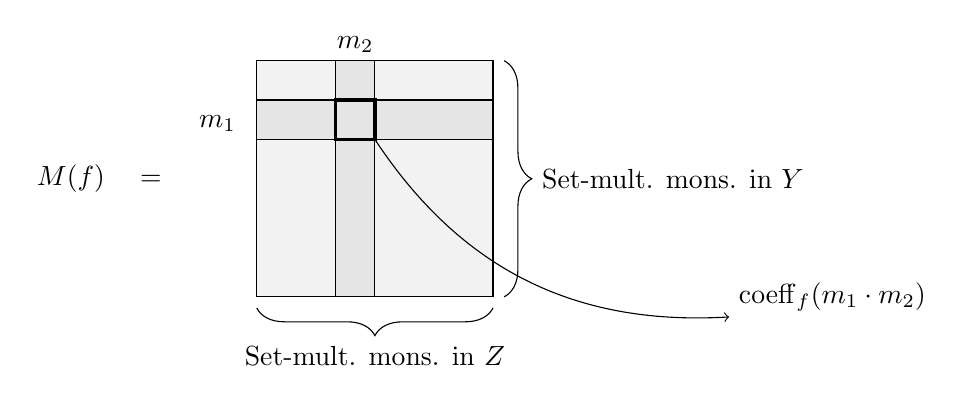
\begin{tikzpicture}
\node at (-2,1.5) {$M(f) \quad= $};
\draw[fill=black!5] (0,0) rectangle (3,3);

\draw[decorate,decoration={brace,amplitude=10pt, mirror, raise=4pt},yshift=0pt]
(3,0) -- (3,3);
\node[anchor=west] at (3.5,1.5) {Set-mult. mons. in $Y$};
\draw[decorate,decoration={brace,amplitude=10pt,mirror, raise=4pt},yshift=0pt] 
(0,0) -- (3,0);
\node[anchor=north] at (1.5,-0.5) {Set-mult. mons. in $Z$};

\draw[fill=black!10] (1,0) rectangle (1.5,3);
\node at (1.25,3.2) {$m_2$};

\draw[fill=black!10] (0,2) rectangle (3,2.5);
\node at (-0.5,2.2) {$m_1$};

\draw[very thick] (1,2) rectangle (1.5,2.5);

\node[anchor=west] at (6,0) {$\mathrm{coeff}_f(m_1 \cdot m_2)$}
edge[<-,bend left] (1.5,2);
\end{tikzpicture}

That is, this is the \emph{communication matrix} when Alice is given all variables of the Alice parts and Bob is given all variables in the Bob parts. The number of rows is $\prod \abs{Y_i}$ and the number of columns is $\prod \abs{Z_i}$. The measures used will be related to the rank of this matrix but it would be convenient to use a normalised version of this, called \emph{relative-rank} (denoted by $\relRank$).
\[
  \mu(f) := \relRank(M(f)) := \frac{\rank(M(f))}{\sqrt{\#\text{rows} \cdot \#\text{cols}}}
\]
Roughly speaking, $\relRank$ is a way of capturing the rank of the matrix and also take into account the \emph{aspect-ratio} of the matrix.

The following are a few simple observations of $\relRank$ that follows readily from the definition.
\begin{observation}[Simple properties of $\mu$]
  The following are some simple properties about the measure $\mu$:
  \begin{enumerate}
  \item \textbf{Trivial upper bound.} For any set-multilinear polynomial $f$, we have
    \[
      \mu(f) \leq \min\inbrace{\sqrt{\frac{\#\text{rows}}{\#\text{cols}}}, \sqrt{\frac{\#\text{cols}}{\#\text{rows}}}}. 
    \]
    In particular, $\mu(f) \leq 1$.
  \item \textbf{Sub-additivity.} For any set-multilinear sum\footnote{That is, $f$ and $g$ set-multilinear with respect to the same parts.} $f+g$, we have
    \[
      \mu(f+g) \leq \mu(f) + \mu(g).
    \]
  \item \textbf{Multiplicativity.} For any set-multilinear product\footnote{That is, $f$ and $g$ set-multilinear on disjoint sub-partitions.}
    \[
      \mu(f \cdot g) = \mu(f) \cdot \mu(g).
    \]
  \end{enumerate}
\end{observation}

To illustrate the key idea, we will illustrate how to get super-polynomial lower bounds for $\Sigma\Pi\Sigma$ circuits, which translates to proving good enough lower bound for set-multilinear $\Sigma\Pi\Sigma\Pi\Sigma$ circuits. 

\subsection{Lower bounds for set-multilinear depth-$5$ circuits}

Until now, we didn't really bother much about the sizes of the parts with Alice and Bob but this will be crucial! Let $k$ be a parameter that is set to $(\log_2 n)/2$ and we will assume that $k > \frac{\sqrt{d}}{2}$.

We will only consider set-multilinear polynomials of degree $d$, where each Alice part $Y_i$ has size exactly $2^{k - \frac{k}{\sqrt{d}}}$ and each Bob part $Z_j$ has size exactly $2^k$. (To avoid the use of floors and ceilings, we will assume that $k$ is divisible by $\sqrt{d}$). However, we will set up the number of Alice parts and Bob parts so that
\[
  \prod \abs{Y_i} \approx \prod \abs{Z_i}
\]
so that the matrix $M(f)$ is almost a square matrix. The imbalance between the sizes of the Alice parts and the Bob parts will be crucial in the proof.\\

The hard polynomial, for now, will be whatever $P$ makes the matrix $M(P) = I$ and hence $\mu(P) = 1$. Noticing that we can actually find an efficiently computable polynomial with $\mu(P) = 1$ is mostly an after-thought and we'll do that later. (TODO)

\subsubsection{Warm-up: Lower bounds for set-multilinear $\Sigma\Pi\Sigma$ circuits}

If $\ell$ is any set-multilinear linear polynomial, then $\ell$ must only involve a single part $X_i$. Therefore,
\[
  \mu(\ell) \leq \frac{1}{\sqrt{\abs{X_i}}}. 
\]
Hence, if $C$ is a size $s$ set-multilinear $\Sigma\Pi\Sigma$ circuit, then
\[
  \mu(C) \leq s \cdot \frac{1}{\sqrt{\abs{X_1} \cdots \abs{X_d}}}
\]

\subsubsection{The lower bound}

\begin{lemma}[Lower bound for set-multilinear depth-$5$ circuits]\label{lem:lb-sml-depth-5}
  Let $f$ be a set-multilinear polynomial with respect to the partition defined above, with $d = o(\log^2 n)$. If $f$ is computable by a size $s$, set-multilinear $\Sigma\Pi\Sigma\Pi\Sigma$ circuit, then
  \[
    \mu(f) \leq s \cdot 2^{-k \sqrt{d}/8}. 
  \]
\end{lemma}

Once we have this lemma, the lower bound is an immediate corollary.

\begin{corollarywp}
  Let $f$ be a set-multilinear polynomial with respect to the above parts with $\mu(f) = 1$. Then, any set-multilinear $\Sigma\Pi\Sigma\Pi\Sigma$ circuit computing it must have size $n^{\Omega(\sqrt{d}}$. 
\end{corollarywp}


\begin{proof}[Proof of \autoref{lem:lb-sml-depth-5}] The proof of this Lemma is embarrassingly simple. Suppose, $C = T_1 +  \cdots + T_r$ where each $T_i$ is a set-multilinear $\Pi\Sigma\Pi\Sigma$ circuit of size $s_i$, then we know that $s \leq \sum s_i$. Thanks to sub-additivity, it suffices to show that $\mu(T_i) \leq s_i \cdot 2^{-k\sqrt{d}/8}$. Hence, let us focus on one such term
  \[
    T = Q_1 \ldots Q_t
  \]
  where (reusing some variables) $T$ has size bounded by $s$ and is a set-multilinear product of set-multilinear $\Sigma\Pi\Sigma$ circuits. Without loss of generality, let $Q_1$ have the largest degree among $Q_1,\ldots, Q_t$.

  \medskip

  {\bf Case 1: $\deg(Q_1) > \sqrt{d}/2$.} In this case, $Q_1$ is a \emph{size-able} factor and hence ``the loss'' from $Q_1$ is going to be sufficient for us.
  \begin{align*}
    \mu(T) & = \mu(Q_1) \cdots \mu(Q_t) \leq \mu(Q_1)\\
           & \leq s \cdot \frac{1}{\sqrt{\abs{X_{i_1}} \cdots \abs{X_{i_{d'}}}}} \leq s \cdot 2^{-\frac{\sqrt{d}}{4} \cdot \inparen{k - \frac{k}{\sqrt{d}}}} \leq s \cdot 2^{-k\sqrt{d}/8}.
  \end{align*}

  \medskip

  {\bf Case 2: $\deg(Q_i) \leq \sqrt{d}/2$ for all $i$.} Since $\mu$ is multiplicative, we have
  \[
    \mu(T)  = \mu(Q_1) \cdots \mu(Q_t).
  \]
  We will show that $\mu(Q_i) \ll 1$ purely from the fact that $M(Q_1)$ will be far from a square matrix!

  Let us focus on one factor $Q$. Suppose this factor depends on $a$ Alice parts and $b$ Bob parts. Further, $a+b = \deg(Q) \leq \sqrt{d}/2$. Let us get a sense of the number of rows and columns in the matrix $M(Q)$.
  \begin{align*}
    \#\text{rows} & = 2^{a \cdot \inparen{k - \frac{k}{\sqrt{d}}}},\\
    \#\text{cols} & = 2^{b \cdot k},\\
    \implies \mu(Q) & \leq \min \set{\sqrt{\frac{\#\text{rows}}{\#\text{cols}}}, \sqrt{\frac{\#\text{cols}}{\#\text{rows}}}}\\
                  & = 2^{- k \cdot \abs{a\inparen{k - \frac{k}{\sqrt{d}}} - bk}} =: 2^{-k \cdot \abs{E}}
  \end{align*}
  where $E = a\inparen{1 - \frac{1}{\sqrt{d}}} - b$. The key point is that $E$ is not close to zero just for the simple reason that the fractional part of $E$ is substantial.

  \noindent
  If $a \leq b$, then $E$ is negative. Hence,
  \begin{align*}
    E & =  a\inparen{1 - \frac{1}{\sqrt{d}}} - b\\
      & \leq \frac{\deg(Q)}{2} \cdot \inparen{1 - \frac{1}{\sqrt{d}}} - \frac{\deg(Q)}{2}\\
      & = \frac{-\deg(Q)}{2\sqrt{d}}.
  \end{align*}
  If $a > b$, then $E$ is positive. There, we have
  \begin{align*}
    E & \geq \{E\} = \inbrace{1 - \frac{1}{\sqrt{d}}}\\
      & > \frac{1}{2} > \frac{\deg(Q)}{4\sqrt{d}}.
  \end{align*}
  Therefore,
  \begin{align*}
    \mu(Q) & \leq 2^{- \frac{k \cdot \deg(Q)}{4\sqrt{d}}}\\
    \implies \mu(T) & = \mu(Q_1)\cdots \mu(Q_t) \leq 2^{-\frac{k \cdot \deg(T)}{4\sqrt{d}}} = 2^{-k\sqrt{d}/4}
  \end{align*}
  And that completes the proof!  
\end{proof}


\subsection{Lower bounds for larger depth}

The lower bound for larger depth proceeds exactly along the same lines (with a few minor technical issues that need to get sorted out). Suppose we are dealing with a depth-$7$ set-multilinear circuit instead. The idea is to proceed exactly along the same lines. Say this circuit $C = T_1 + \cdots + T_r$, it suffices to focus on each summand $T_i$. Suppose such a summand $T = Q_1 \cdots Q_t$ where each $Q_i$ is now a set-multilinear depth-$5$ circuit.

{\bf Case 1: $\deg(Q_1)$ is large.} In this case, just use the upper-bound we just proved for set-multilinear depth-$5$ circuits to bound $\mu(Q_1)$ and hence $\mu(T)$.

\medskip

{\bf Case 2: All $\deg(Q_i)$'s are small.} Use the same argument to show that each $M(Q_i)$ is non-square-ish to get the upper bound on $\mu(Q_i)$ and hence $\mu(T)$.\\

The only technical hurdle is that earlier we had chosen our $k$ depending on what degree we were working with etc. but now the choice needs to be flexible. Fortunately, there is a lot of room in the choice of the parameter $k$ and this allows essentially the same argument to sail through without too much difficulty. That's basically the proof for arbitrary constant depth as well. 


\section{TODO: Subsequent results}

There were some subsequent results proved by the Limaye, Srinivasan and Tavenas that ought to be added here. Some of these include:
\begin{itemize}\itemsep0pt
\item Super-polynomial separation between depth $\Delta$ and depth $\Delta+1$
\item Super-polynomial separation between homogeneous formulas and algebraic branching programs in the non-commutative setting
\end{itemize}





%%% Local Variables: 
%%% mode: latex
%%% TeX-master: "fancymain"
%%% End: 



\bibliographystyle{customurlbst/alphaurlpp}
\bibliography{references,crossref}

%%% Local Variables: 
%%% mode: latex
%%% TeX-master: "fancymain"
%%% End: 
